%\documentclass[10pt,twocolumn]{article}
\documentclass[a4paper,12pt,openany]{book}

\usepackage{graphicx}% Include figure files
\usepackage{setspace}
\usepackage{dcolumn}% Align table columns on decimal point
\usepackage{bm}% bold math
\usepackage{amsmath}
\usepackage{hyperref}
\usepackage{caption}
\usepackage{listings}
\usepackage{float}
\usepackage{hyperref}
\usepackage{lscape}
\usepackage{wallpaper}
\usepackage{color}
\usepackage{geometry}
\usepackage{minted} 
\usepackage{datetime}
\usepackage{titlesec}
\usepackage{wrapfig}
\usepackage{makeidx}
\usepackage{subfig}
\usepackage{mwe}
\usepackage{wrapfig}
\usepackage{lipsum}
\usepackage[shortlabels]{enumitem}
\makeindex

%Counters
\newcounter{question}
\setcounter{question}{0}

%names of the model
\newcommand{\simname}{OghmaNano}

\newcommand{\fileext}{.oghma}
\newcommand{\coreexename}{\emph{oghma\_core.exe}}
\newcommand{\guiexename}{\emph{oghma.exe}}
%\providecommand{\e}[1]{\ensuremath{\times 10^{#1}}}

\newdateformat{monthdayyeardate}{%
  \monthname[\THEMONTH]~\THEDAY, \THEYEAR}

\geometry{a4paper,margin=20mm,heightrounded,}

\linespread{1.0}


\begin{document}


\color{white}
%\title{\Huge \textbf{gpvdm user manual v7.88+}}

%\author{\textbf{Roderick C. I. MacKenzie}\\
%\\
%\textbf{roderick.mackenzie@durham.ac.uk}
%}

%\addtolength{\wpXoffset}{-10cm}
%\CenterWallPaper{2.15}{./images/trent.jpg}

%\centerline{\textbf{roderick.mackenzie@durham.ac.uk}}

%\maketitle

\begin{titlepage}
   \vspace*{\stretch{1.0}}
   \begin{center}
      \Huge\textbf{Understanding gpvdm v7.88+}
   		\vspace{\stretch{0.1}}
   \end{center}

   \begin{center}
      \large\textbf{Roderick C. I. MacKenzie}
   		\vspace{\stretch{0.01}}
   \end{center}

   \begin{center}
      \large\textbf{\monthdayyeardate\today}
   \end{center}
   \vspace{\stretch{0.1}}
   \begin{center}
      \large\textbf{roderick.mackenzie@durham.ac.uk}
   \end{center}

   \vspace*{\stretch{8.0}}
\addtolength{\wpXoffset}{-10cm}
\CenterWallPaper{2.15}{./images/trent.jpg}
\end{titlepage}

\newcounter{question}
\setcounter{question}{0}

\pagenumbering{gobble}



\color{black}

%\begin{figure}[ht!]
%\centering
%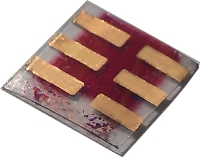
\includegraphics[width=30mm]{./images/cell.jpg}
%\label{overflow}
%\end{figure}

\newpage

\ClearWallPaper

\vspace*{\fill}
Please do not cite this manual.  Please see the section \ref{sec:using_gvpdm} on how to cite the model in your work.
\vspace*{\fill}


Front cover: A picture of a thermal power station in \href{https://en.wikipedia.org/wiki/Ratcliffe-on-Soar_Power_Station}{Ratcliffe-on-Soar} Nottinghamshire taken on a cold January afternoon in 2017. Most of the emissions you see in the image is water from the cooling towers however the gasses rising form the tall thin chimney on the left hand side of the image are the products of burning hydrocarbons which previously buried in the ground for about 300 million years.


\chapter{Introduction}
\section{What is OghmaNano?} 
OghmaNano officially stands for \emph{\textbf{O}r\textbf{g}anic and \textbf{h}ybrid \textbf{M}aterial \textbf{N}ano Simulation tool}.  Oghma is also the name of the \href{https://en.wikipedia.org/wiki/Ogma}{Gaelic God} who's appearance is described as "sun-faced" or "shining/radiant", he is creditied with developing \href{https://en.wikipedia.org/wiki/Ogham}{Ogham}, the script in which Irish Gaelic was first written. The creators of OghmaNano spent a lot of time making sure it can describe the light and optical radiation correctly thus the name seems like a good fit. How you remember the name is up to you.

OghmaNano was originally developed to be a general purpose model for simulating photovoltaic devices, including organic and perovskite cells. However, since its initial development the model has expanded to simulate many other classes of optoelectronic devices including, Organic Light Emitting Diodes (OLEDs), Organic Field Effect Transistors (OFETs), large area printed devices, optical filters, photonic crystals and many more.  In general OghmaNano can simulate any opto-electronic-device where electrons, photons (and also heat - phonons) interact.  The model has been downloaded by thousands of people across the globe (see figure \ref{fig:downloadmap}) and is used in many top universities and companies. Figure \ref{fig:alldevices} shows some of the classes of devices OghmaNano can simulate.  Key features of OghmaNano are listed below:

\begin{itemize}
  \item Electrical models:
  \begin{itemize}
    \vspace{-0.2cm}\item 1/2D electrical drift-diffusion solver.
    \vspace{-0.2cm}\item Dynamic SRH traps needed for simulating disordered materials.
    \vspace{-0.2cm}\item Simple equivalent circuit model.
    \vspace{-0.2cm}\item Complex 3D circuit model for complex large area devices.
    \vspace{-0.2cm}\item Arbitrary user defined densities of trap states.
    \vspace{-0.2cm}\item Thermal model linked to the electrical models.
    \vspace{-0.2cm}\item Time domain, frequency domain and steady state solvers.
  \end{itemize}
  \item Optical models:
  \begin{itemize}
    \vspace{-0.2cm}\item Transfer matrix model for light
    \vspace{-0.2cm}\item FDTD models
    \vspace{-0.2cm}\item Ray tracing model
    \vspace{-0.2cm}\item 1/2D optical mode solvers for waveguide structures.
    \vspace{-0.2cm}\item Arbitrary light sources/filters.
  \end{itemize}
  \item Excited states/mobile ion:
  \begin{itemize}
    \vspace{-0.2cm}\item 1/2/3D Exciton solver.
    \vspace{-0.2cm}\item Excited singlet/triplet state solver.
    \vspace{-0.2cm}\item Mobile ions, doping and tunneling through interfaces.
  \end{itemize}
  \item Other/databases:
  \begin{itemize}
    \vspace{-0.2cm}\item Comprehensive materials databases.
    \vspace{-0.2cm}\item Ability to convert arbitrary shapes to 3D objects.
    \vspace{-0.2cm}\item Comprehensive 3D shape database.
  \end{itemize}
\end{itemize}

\section{Why OghmaNano?}
\begin{minipage}{0.5\textwidth}
By burning fossil fuels we are releasing $\sim 33.3$ gigatonnes of $CO_2$ per year \cite{Liu2022} and thus humanity is steadily changing the composition of Earth's atmosphere. Since 1960, $CO_{2}$ in the atmosphere has risen by around \href{https://gml.noaa.gov/ccgg/trends/}{30\%} this in turn is increasing average global temperatures\cite{ManabeandWetherald} and making our home planet Earth, a more difficult place to live on. We therefore have two choices, either cut emissions or face an existential crisis.

Thin film devices such as solar cells and OLEDs offer a viable way to reduce our $CO_{2}$ emissions, either by providing low carbon electricity, or providing an efficient way to use the energy once generated.

\end{minipage}
\hspace{4pt}
\begin{minipage}[]{0.5\linewidth}
\centering
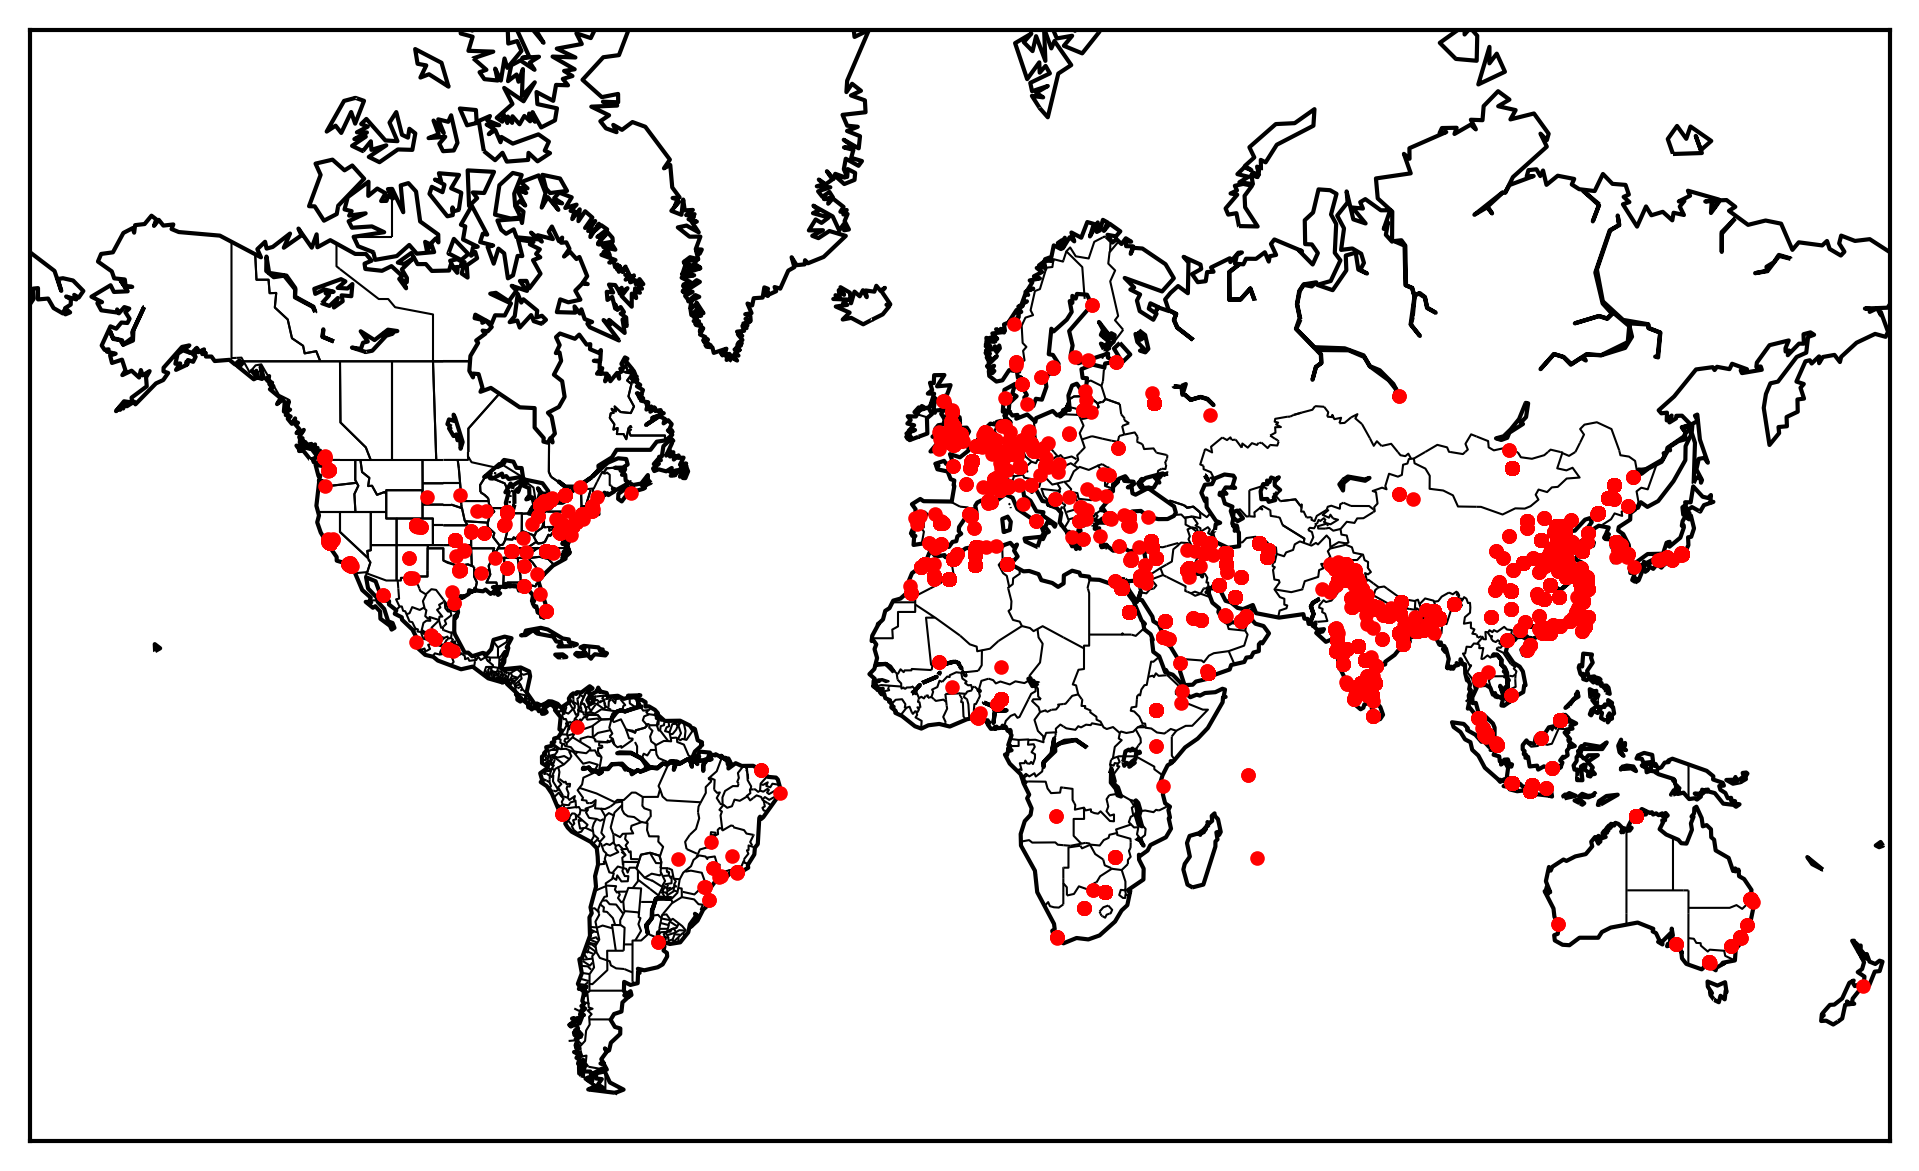
\includegraphics[width=\textwidth]{./images/map.png}
\captionof{figure}{A map of locations where OghmaNano has been downloaded.}
\label{fig:downloadmap}
\end{minipage}

  It is therefore important that technologies based on thin film devices continue to be developed and succeed. By developing and releasing OghmaNano, I hope, I am enabling scientists throughout the world to understand these devices a little bit better, which I hope will contribute in a very small way to solving our climate crisis.

Solar cells and OLEDs happen to come from a class of devices called diodes. This class of devices has many uses including optical sensors, medical sensors, switches, rectifiers. Thus as a pleasant side effect of OghmaNano the development of these devices is also being helped. 

\begin{figure}
\centering
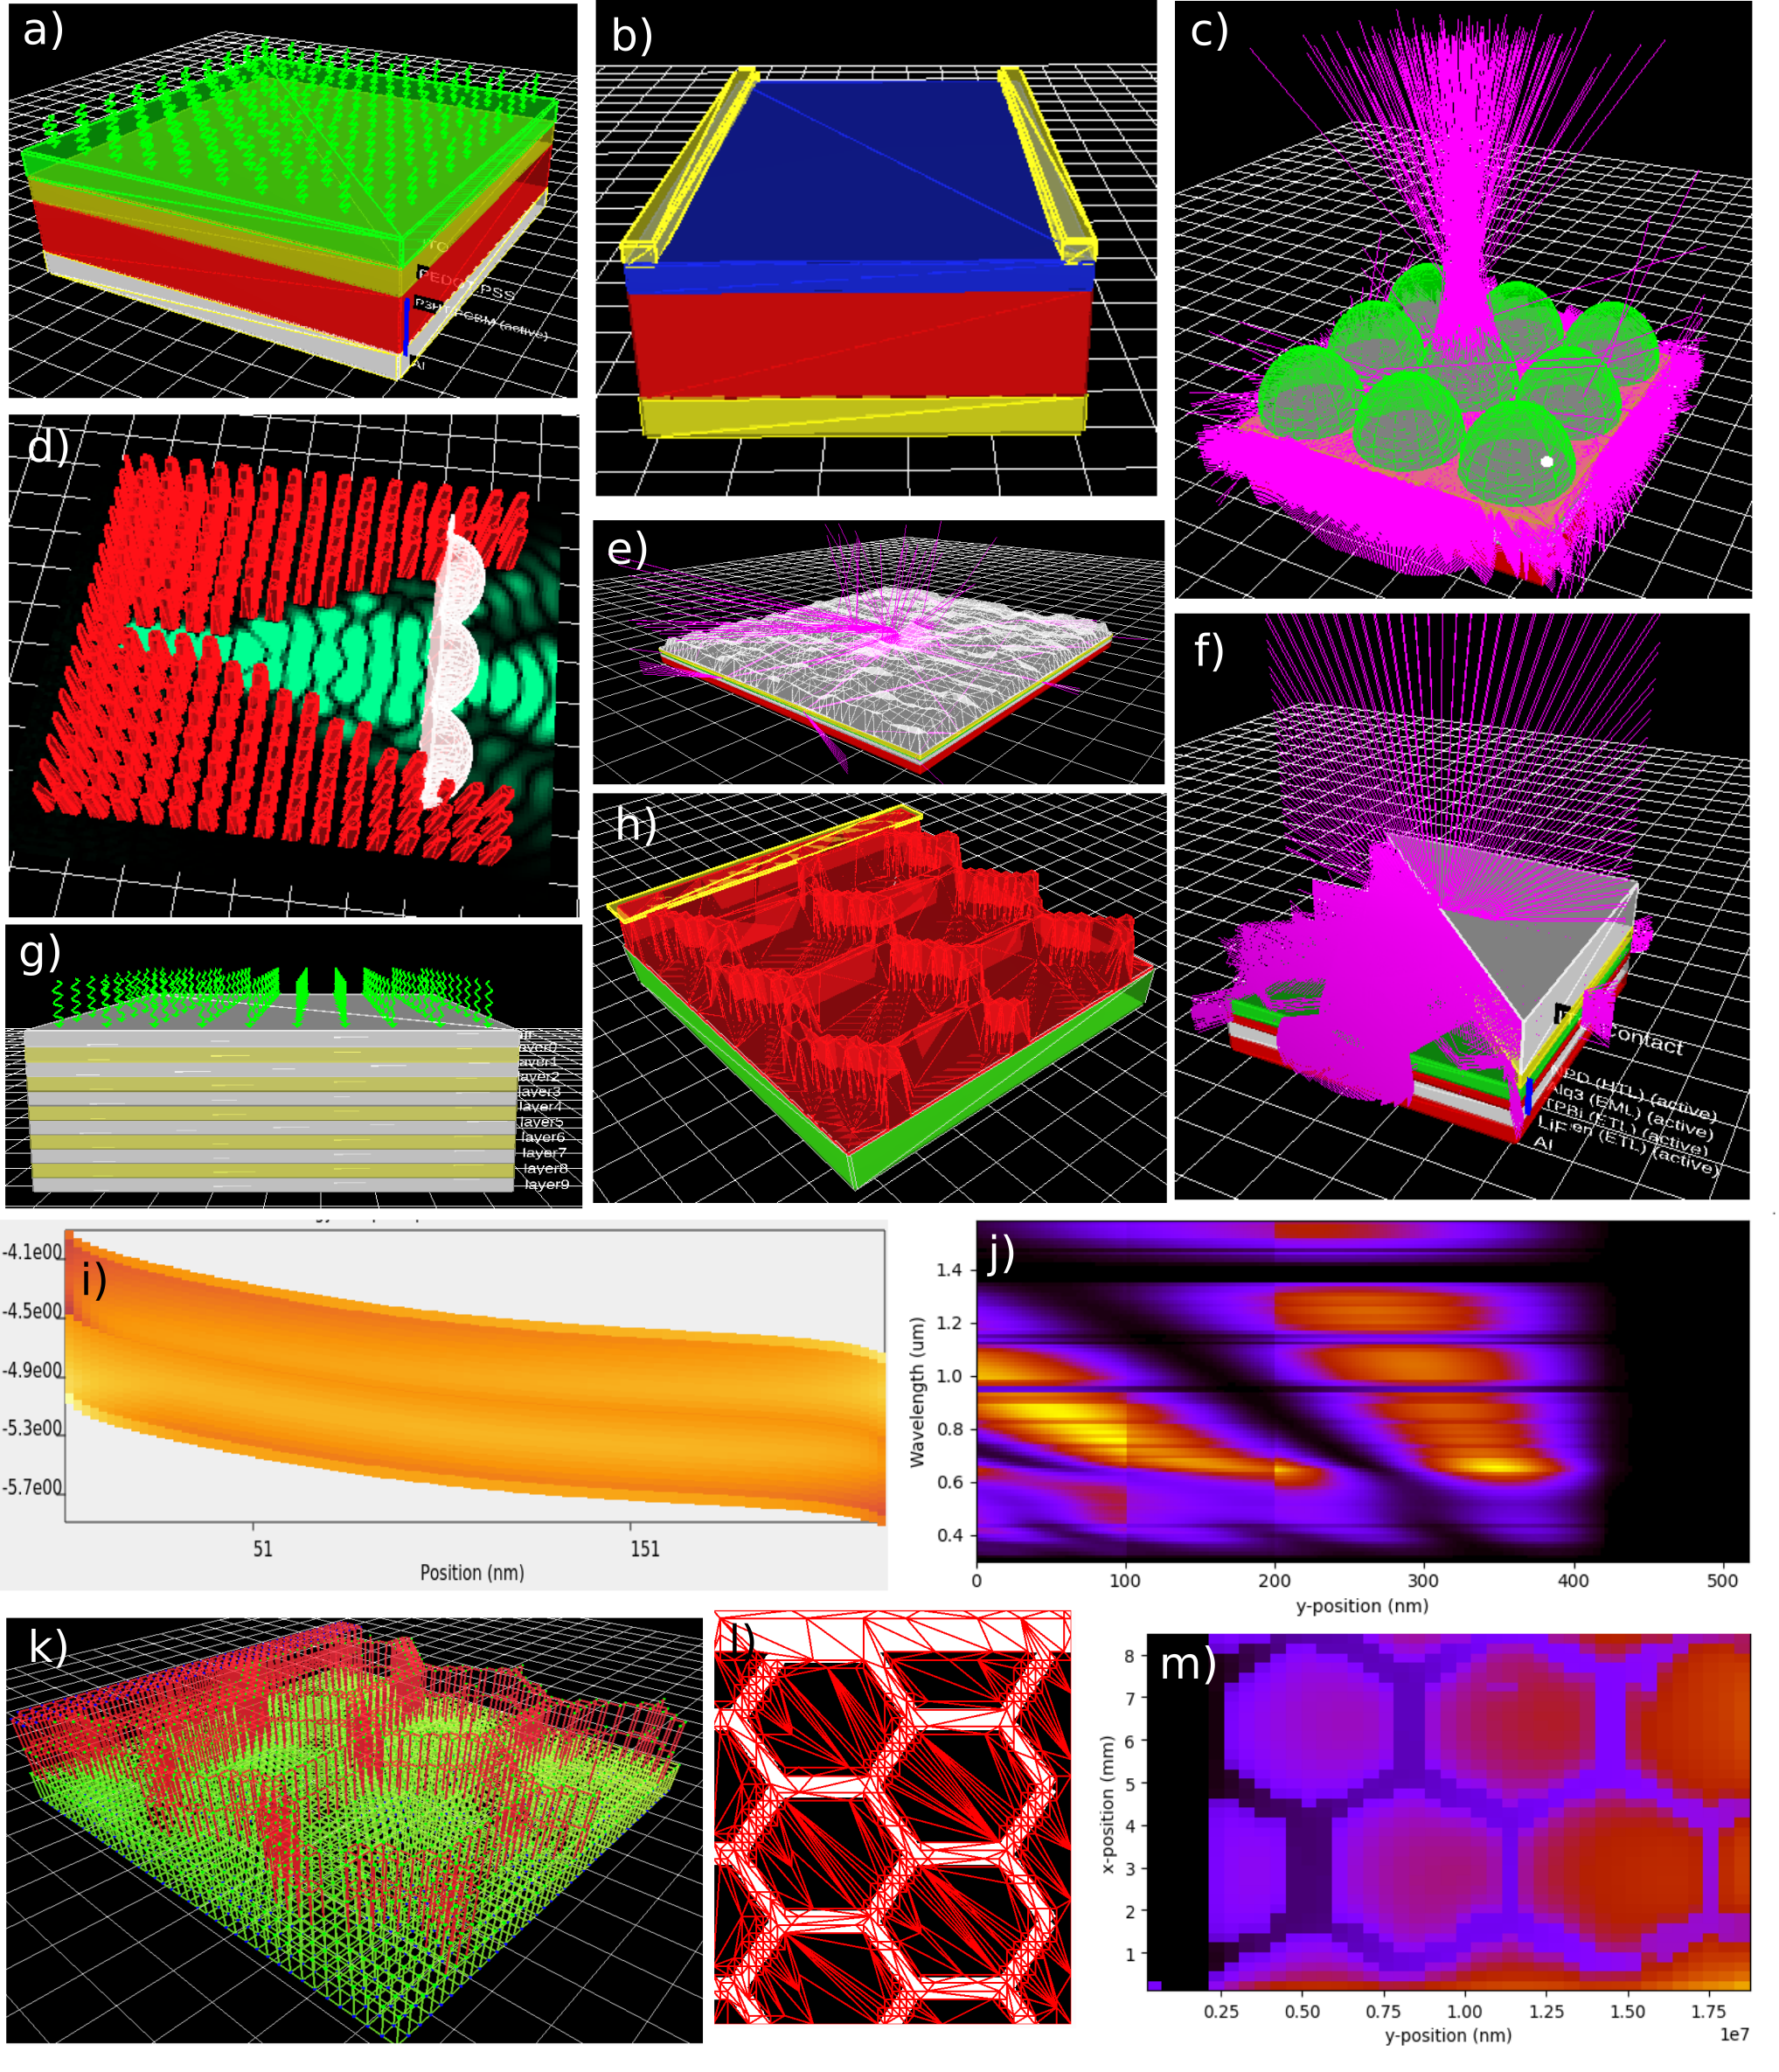
\includegraphics[width=0.9\textwidth]{./images/all_devices.png}
\caption{a); Organic/Perovskite solar cell simulation; b) OFET transistor simulation; c) Microlens simulation; d) Photonic waveguide simulation; e) light escaping structured films; f) OLED simulation; g) Optical filter simulation; h) large area device modelling (hexogonal contacts); i) Mapping carrier density in position/energy space; j) Building complex 3D meshes; and k) resistance maps of large area devices.}
\label{fig:alldevices}
\end{figure}



\section{About this book/manual}
This book is intended to be the definitive guide to simulating devices with OghmaNano. The idea is that one can read this book and learn in a step-by-step way how to simulate many modern opto-electronic devices with very limited prior knolage.  However, not all aspects of this book are yet finished. I therefore recommend you also watch the \href{https://www.youtube.com/channel/UCbm_0AKX1SpbMMT7jilxFfA}{YouTube} channel (and subscribe! ;)) where I describe many of the features in more detail and give demonstrations on the use of the model. I would suggest you treat the videos as lectures (and take notes) rather than entertaining videos (well I hope they are entertaining too!). New releases are generally announced on \href{https://twitter.com/OghmaNano}{Twitter}, which I also suggest you follow to make sure you are using an up-to date version. I often release version every week, a version that is 6 months old is considered very old indeed.  Please read papers which were published from this model - do also read the supplementary information (SI) to the papers, as I often write about the model in there.
This book starts off with explaining how to simulate organic solar cells. This is because organic solar cells are the easiest class of device to simulate, it then moves onto Perovskite devices, and OLEDs. More complex classes of devices follow.  If you are new to simulation work or in indeed OghmaNano, I suggest you start with the first chapters and work your way to the more complex devices.

\section{What is the history of OghmaNano?}
I started writing OghmaNano just after finishing my PhD in 2009 while taking a break for academia and deciding what to do next. At that time it was a simple 1D drift-diffusion diode model designed to simulate solar cells which did not take account of disorder.  Over the next 14 or so years the model has been significantly expanded to model many classes of material system and classes of devices. Since 2009 thousands of people have downloaded OghmaNano and \href{http://www.Oghma-Nano.com/publications.html}{hundreds (the list is by definition always out of date)} of people have published their own papers using the model. If you publish with OghmaNano let me know and I will update the list to include your paper.

\section{What is the roadmap for OghmaNano?}
The aim is to make OghmaNano a completely general opto-electronic model which can be used by anyone to learn about and explore the world of novel opto-electronic devices.  I want OghmaNano to be an engine which people can use to push their own research forward and for education. The exact road map on how to get there is not defined.  As collaborators contact me asking for new features I add them, what comes first depends on what people want.. I never view OghmaNano as finished, and release improvements in small increments, therefore if you discover and report a bug, check back in a week or so to see if it is fixed in the next version.  The same goes for this book, it evolves weekly as I write it. So if a section is missing, check back next week it might be finished.

\section{Using OghmaNano in industrial/academic work}
\label{sec:using_gvpdm}
You are free to use OghmaNano in industrial/academic work. In fact, I'm happy if you do so. However, the following conditions apply:
\begin{enumerate}
  \item If you use OghmaNano to generate results, then clearly say so in your work. This can be as simple as one sentences saying: "we used OghmaNano to perform the simulations"
  \item If you publish a book, paper or thesis where OghmaNano has been used you must cite at least three papers associated with the model.  To find out which papers to cite, click on the area indicated in red in figure \ref{fig:cite_me} when using the model. PLEASE do not cite the manual. I can't include the manual in paper lists when applying for funding.
\end{enumerate}

I ask you to do this because citations are an easy way to demonstrate that people are using OghmaNano. Demonstrating use is key to finding money/people to continue the development of OghmaNano.  So by doing this you are guaranteeing the future of OghmaNano and its continued availability for others.  Thank you!


\begin{figure}
\centering
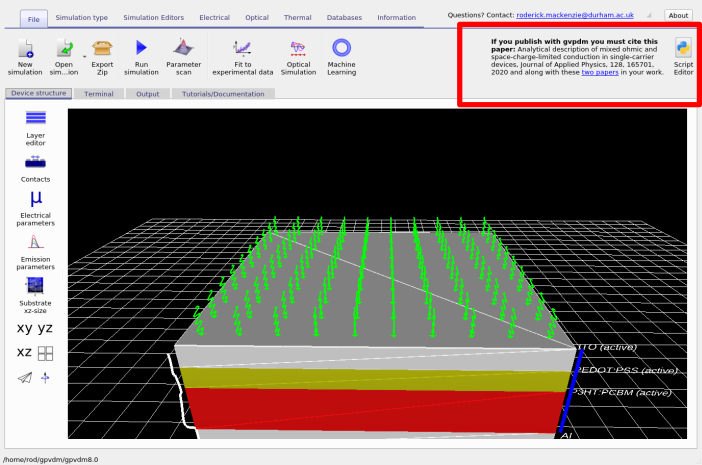
\includegraphics[width=0.7\textwidth]{./images/cite_me2.png}
\caption{If you click on the area indicated by the red box, the model will tell you which papers should be cited.}
\label{fig:cite_me}
\end{figure}

\section{Bugs}
I get quite a lot of feature requests from people wanting features added or for bugs to be fixed. I really appreciate the feedback!  However, I am currently employed at a UK University and my time is split between teaching, research and admin. My performance in my job is measured by the number of high impact papers I push out per year. I therefore have to prioritize feature requests and bug fixes for people who would like to write a paper with me (i.e. my collaborators).... Therefore if you would like:

\begin{itemize}
  \item A bit of advice on how to do x or y with the model then please do feel free to shoot me a mail, and I will do my best to get back to you. If you don't hear back from me just send the mail again.. I get loads of e-mails, and things get lost if I don't answer quickly.
  \item If you want to report a bug, then please do that, and I will do my best to fix it in the next release. But I can't promise when it will be fixed.
  \item  If you would like a features added or a steady stream of help (i.e. you are asking for my time) then please consider inviting me to join in your work and collaborate on a joint paper. I am happy to add whatever feature you want to the model, or fix what ever bug you may have but in return I would ask for the inclusion of my name on the author list. By doing this it makes it much easier for me to justify sinking time into your project.
\end{itemize}
    
If you don't need help from me to use OghmaNano then please feel free to do what you want with the results - no need to contact me, but do cite it correctly.



\chapter{Installing OghmaNano}

\section{Windows (if you have admin rights)}
Go to the download page for OghmaNano at \url{http://www.Ogham-Nano.com/windows.php} and download the latest version.  Simply double click on it and say yes to all questions, it will then install on your PC and an icon will appear in the start menu. I recommend you install it in the default directory.

In general I release a new version every couple of weeks and it's worth keeping your version up-to-date. On modern versions of windows, windows will ask you if you want to install an unsigned executable from an unknown author, and warn you that this could damage your computer.  The reason you get this message is because I have not cryptographically signed the .exe file. I have not signed it because I do not own a private cryptographic key with which to do this.  To get such a key I would have to send my passport off to a key authority to prove who I am and then pay them 500 pounds/year for the privilege of them validating who I am.  Needless to say, that I am not very excited about paying 500 pounds/year so you will just have to click away the warnings from windows.

\section{Windows (No admin rights)}
If you don't have admin rights to your computer it can be hard to install new software, OghmaNano offers the option of running OghmaNano while not properly installed.  Download the zip file containing OghmaNano from \url{https://www.Oghma-Nano.com/download_no_admin.php}.  Once you have downloaded the zip archive, open the zip file and extract the folder $pub$ to c:\textbackslash . Then rename the folder to be called c:\textbackslash OghmaNano.  Once you have done this run the executable c:\textbackslash OghamNano\textbackslash OghmaNano.exe (see figure \ref{fig:directory}).

\begin{figure}
\centering
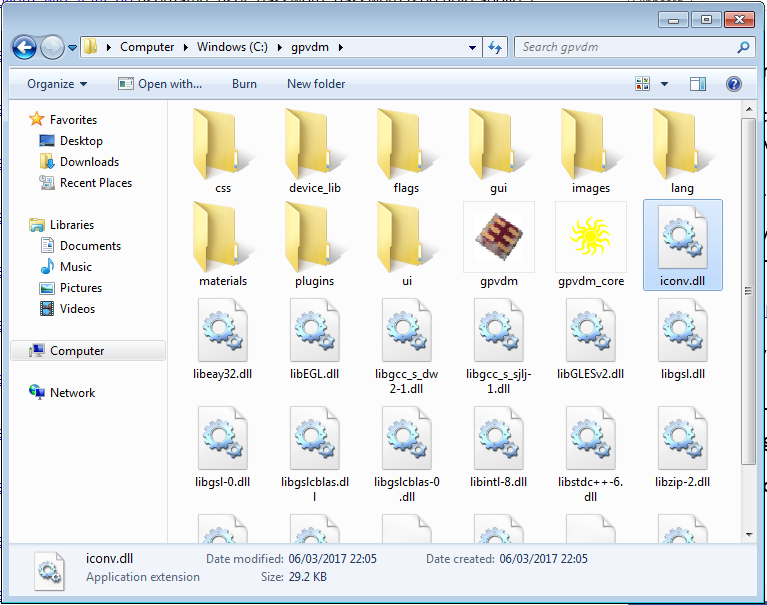
\includegraphics[width=70mm]{./images/dir.png}
\caption{Running and installing OghmaNano.  Double click on the OghmaNano icon to run the model.}
\label{fig:directory}
\end{figure}

%\section{Linux} \label{installing_on_linux}
%The windows version of OghmaNano seems to be much more popular than the Linux version.  Therefore, I will tend to publish an updated windows exe every couple of weeks (along with the platform independent source code) and only publish updated linux rpms/deb packages when someone asks me to.  This means that the Linux deb/rpm files tend to lag behind the windows version by about a year.  For this reason I recommend you install the Linux version from source.


%\subsection{Linux from source the easy way}
%Download the OghmaNano by issuing the command

%\begin{verbatim}
%git clone  https://github.com/roderickmackenzie/gpvdm
%\end{verbatim}
%Find your operating system in

%\begin{verbatim}
%build_system/dependency_scripts
%\end{verbatim}

%This script should install all the packages you need to run/compile OghmaNano for a given OS. I don't always keep them up to date, so if you have a new version of an OS and the packages have been renamed you may have to hunt around.

%Then run:
%\begin{verbatim}
%./build
%\end{verbatim}

%Then select, (compile), and (auto). Then hit return to build.


%\begin{figure}[H]
%\centering
%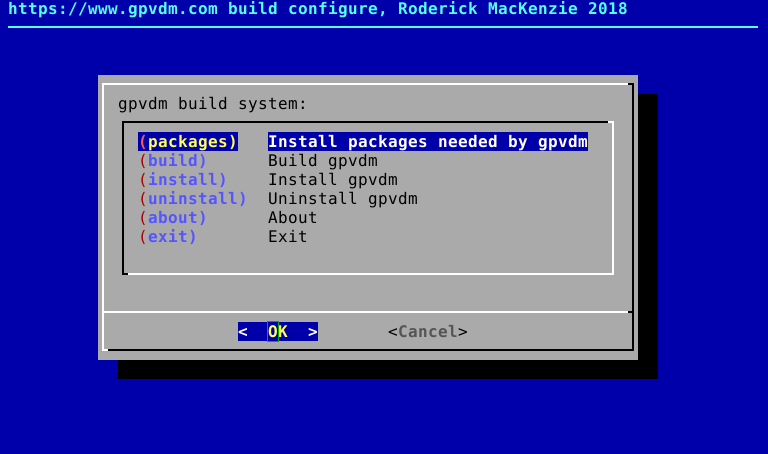
\includegraphics[width=0.7\textwidth]{./images/build.png}
%\caption{The linux build system, run ./build to get this menu.  }
%\label{fig:build}
%\end{figure}


%%%%%%%%%%All elecctrical stuff
\chapter{Getting started}
\section{Simulating a JV curve of a simple solar cell}
\begin{minipage}{0.5\textwidth}
No matter which type of device you want to simulate, if you are new to OghmaNano my advice is to start off with this organic solar cell simulation. Organic solar cells are by far the most simple class of device you can simulate, and will let you understand the basics of the package without having to deal with 2D effects, perovskite ions of light emission.  This chapter will guide you through your first organic solar cell and explain the nuts and bolts of running simulations with OghmaNano. Once installed OghmaNano appear on the start menu, click on it to launch it. Once run, a window resembling that in figure \ref{fig:new_open} will appear.
\end{minipage}
\hspace{4pt}
\begin{minipage}[]{0.5\linewidth}
\centering
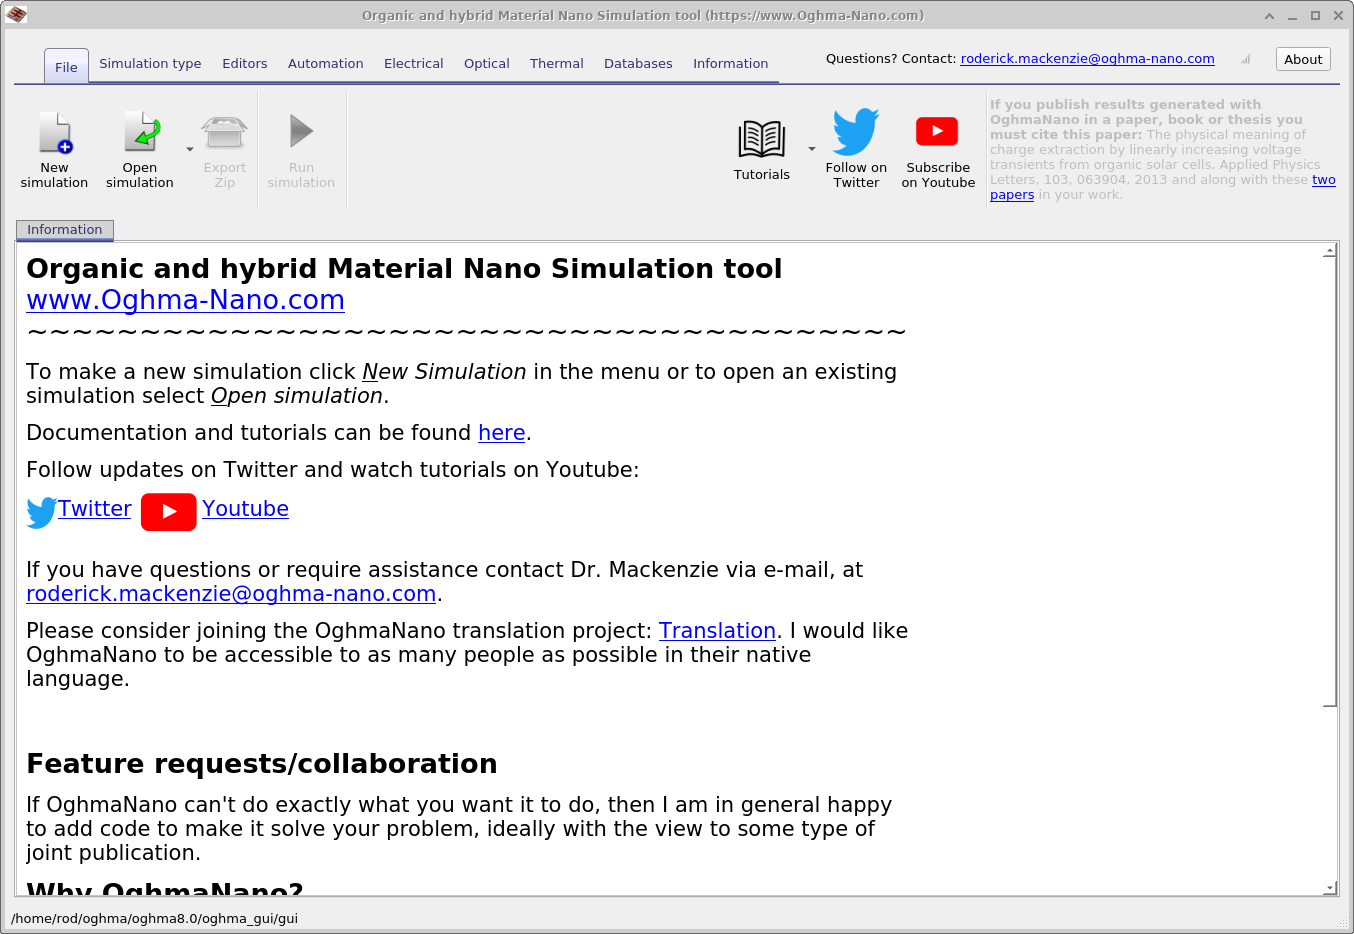
\includegraphics[width=\textwidth,height=0.7\textwidth]{./images/running/new_open.png}
\captionof{figure}{The main OghmaNano simulation window.}
\label{fig:new_open}
\end{minipage}

\subsection{Making your first simulation}

Click on the $new~simulation$ button.  This will bring up the new simulation window (see figure \ref{fig:new_new}). From this window double click on the $Organic~Solar~Cells$ icon. This will bring up a sub menu of different types of Organic Solar cells (see figure \ref{fig:new_opv}). The majority of these device simulations have been published in papers and calibrated to real organic solar cells. The oldest is the (non-inverted) P3HT:PCBM device from 2012 \cite{mackenzie2012extracting} and the newest are the PM6:Y6 devices from 2022 \cite{zhu2022single,wopke2022traps}. \emph{Double click on the P3HT:PCBM simulation for this example and save the new simulation to disk.}

Once you have saved the simulation, the main OghmaNano simulation window will be brought up (see figure \ref{fig:simpleinterface}). You can look around the structure of the solar cell, by dragging the picture of the solar cell with your mouse.  Try pressing on the buttons beneath the red square, they will change the orientation to the \emph{xy}, \emph{yz} or \emph{xz} plane. Notice the x,y,z origin marker in the bottom left of the 3D window. The icon with four squares will give you an orthographic view of the solar cell.


Click on the button called \emph{Run simulation}, to run the simulation (hint it looks like a blue play button and is located in the \emph{file} one to the right of the "Simulation type ribbon" ).  The function key F9 will also run the simulation. On slower computers it could take a while. Once the simulation is done, click on the $Output$ tab (see figure \ref{fig:output}), there you will see a list of files the simulation has written to disk.

\noindent
\begin{minipage}{0.45\textwidth}
\centering
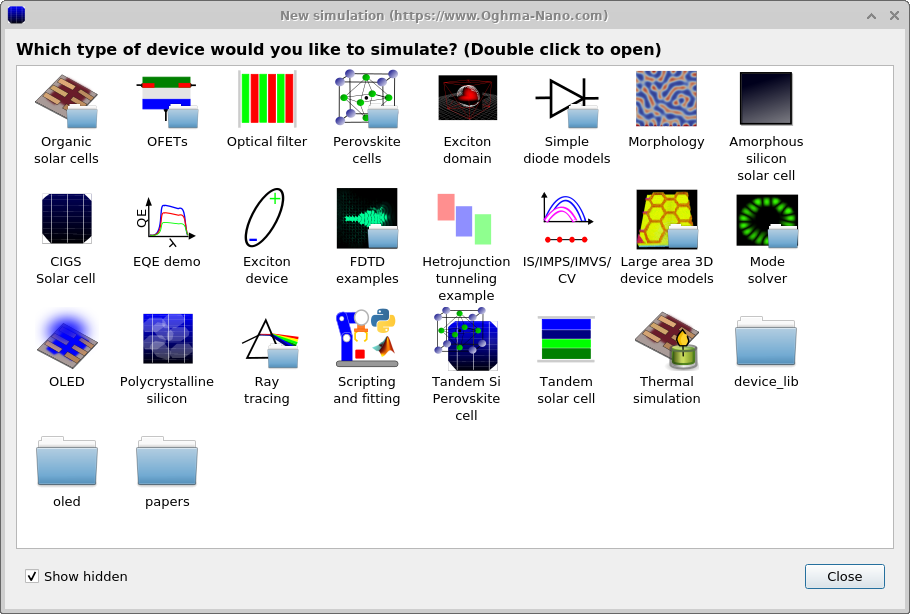
\includegraphics[width=\textwidth,height=0.7\textwidth]{./images/running/new.png}
\captionof{figure}{New simulation window, from here you can select different example simulations. It is often easier to start from a base simulation rather than build your own from scratch.}
\label{fig:new_new}
\end{minipage}
\hspace*{10px}
\begin{minipage}[]{0.45\linewidth}
\centering
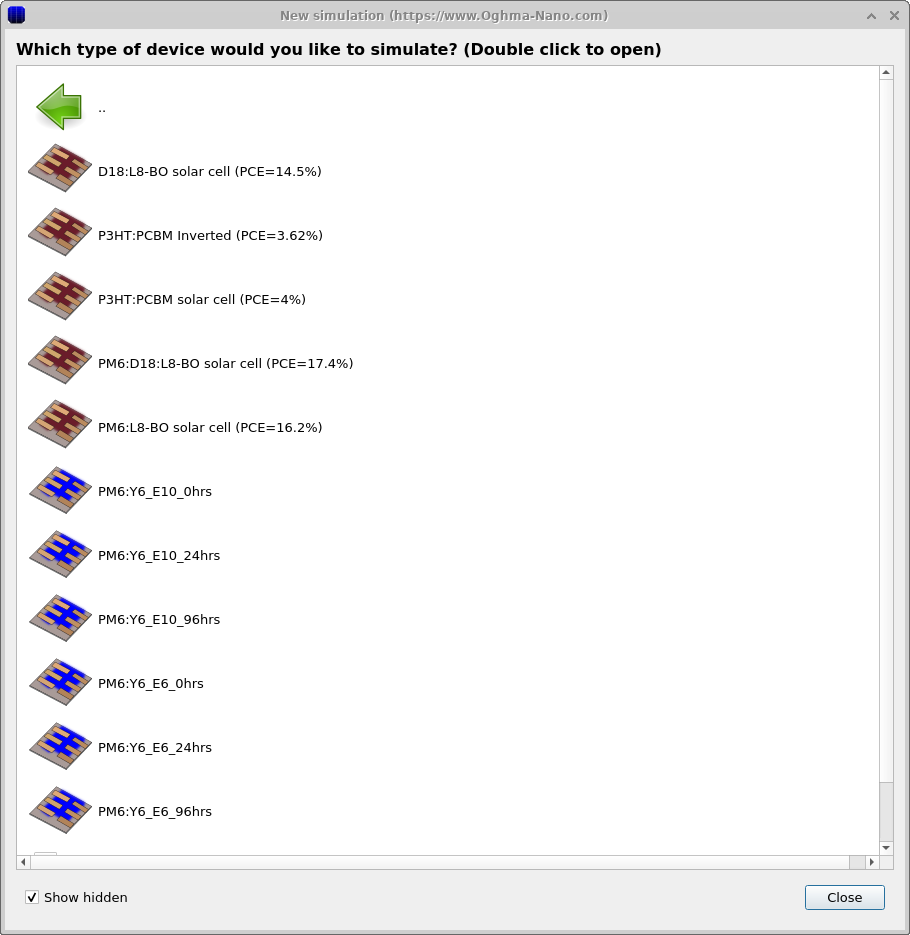
\includegraphics[width=\textwidth,height=0.7\textwidth]{./images/running/new_opv_device.png}
\captionof{figure}{The organic solar cell sub menu. There are quite a few examples of organic solar cells in this menu. The majority of simulations have been used to produce papers \cite{mackenzie2012extracting,zhu2022single,wopke2022traps}.}
\label{fig:new_opv}
\end{minipage}


\subsubsection{What's the best place to save your simulation?}
OghmaNano dumps a lot of data to disk, I therefore recommend you save the simulation to a local disk such as the C:\textbackslash drive, a network drive or USB stick drive will be far too slow for the simulation to run.  I would also not save the simulation onto OneDrive or Dropbox as they are also too slow and saving it there will generate a lot of network traffic.  If you are a power user doing a lot of fitting of experimental data I would also recommend (at your own risk(!)) disabling any extra antivirus software you have installed, as quite often the antivirus software can't keep up with the read/writes to disk.

\begin{figure}[H]
\centering
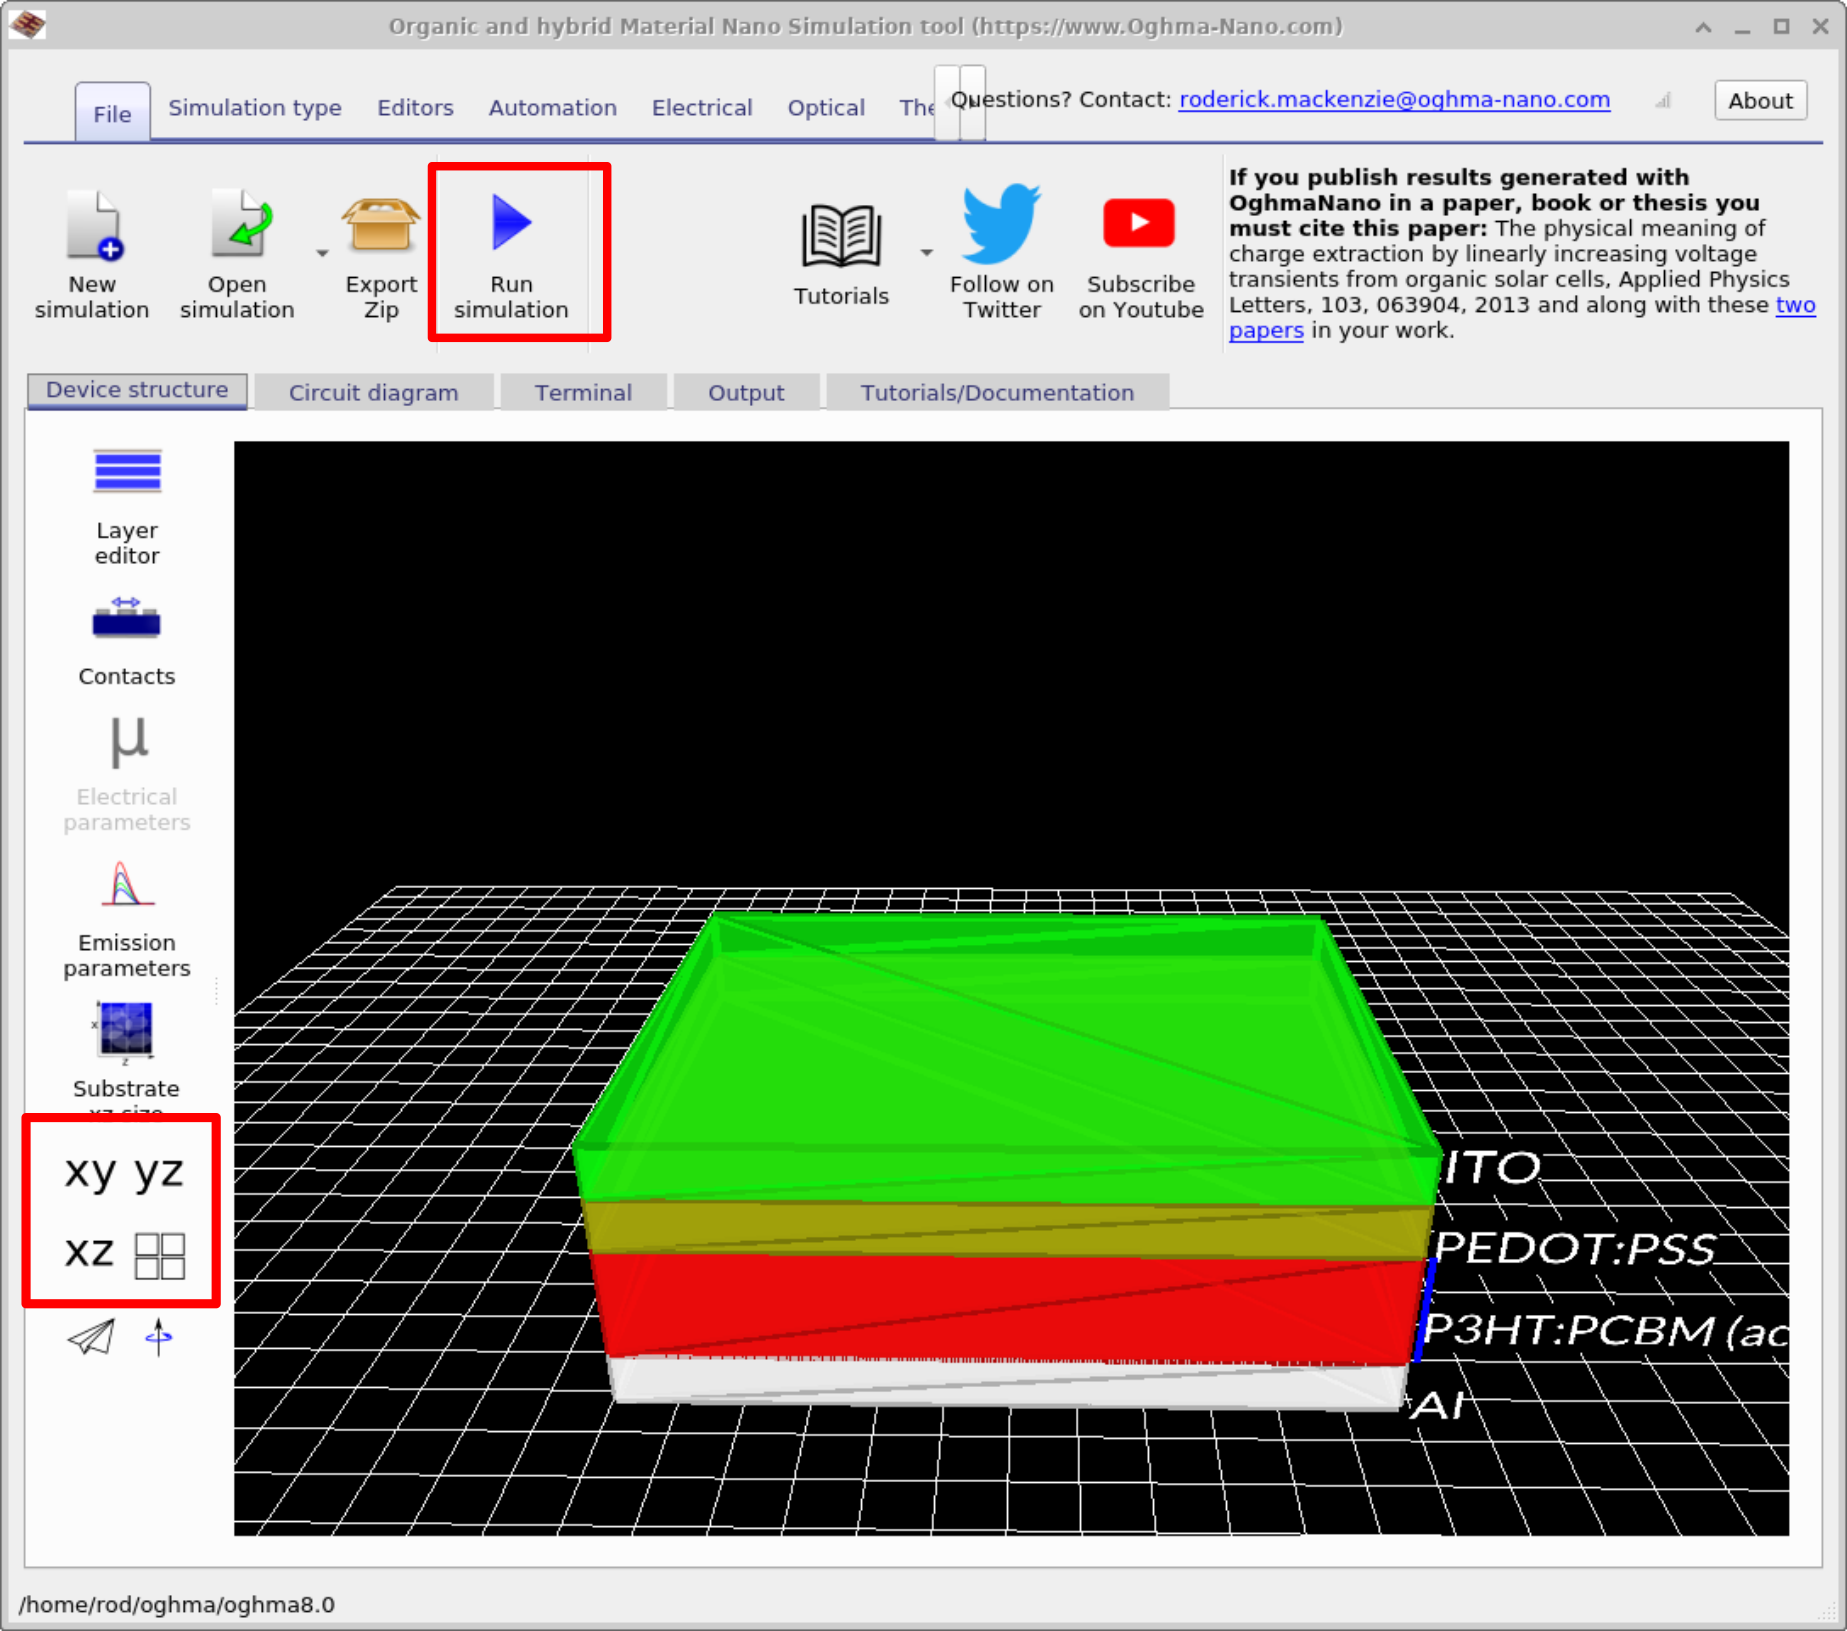
\includegraphics[width=0.8\textwidth,height=0.5\textwidth]{./images/running/simple_interface.png}
\caption{The main OghmaNano simulation window with the xy, yz and xz buttons visible. The play button is also visible which is used to run the simulation, the function key F9 can also be used to run the simulation.}
\label{fig:simpleinterface}
\end{figure}






\pagebreak
\subsection{The output from your first simulation}

After you have clicked on the \emph{Run Simulation} button (or pressed the function key F9) to run the simulation, the results from the simulation will have been written to disk. To view these results click on the \emph{Output} tab in the main window. There you will see the output from the simulation, this is visible in figure \ref{fig:output}
\begin{figure}[H]
\centering
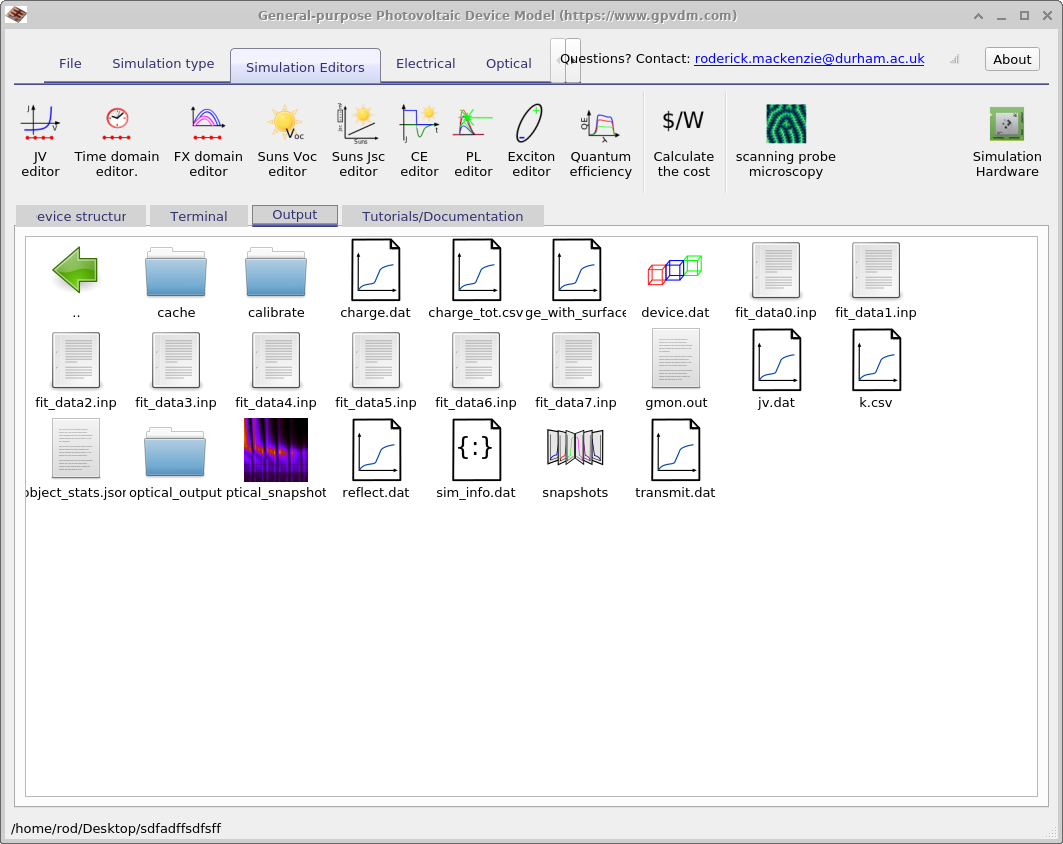
\includegraphics[width=0.6\textwidth,height=0.5\textwidth]{./images/running/output.png}
\caption{The \emph{Output} tab this is just like windows file explorer, you can explore the simulation directory tree.}
\label{fig:output}
\end{figure}


Key files the simulation produces are listed in the table below:

\begin{table}[H]
\begin{center}
\begin{tabular}{ |c|c|c| } 
 \hline
	File name 			& 	Description  \\ 
 \hline
	$jv.dat$ 			&	Current v.s. voltage curve \\ 
	$charge.csv$ 		&	Voltage v.s. charge density curve\\ 
	$device.dat$ 		&	The 3D device model\\ 
	$fit\_data*.inp$ 	&	Experimental data for this device.\\
	$k.csv$ 			&	Voltage v.s. Recombination constant k\\ 
	$reflect.csv$ 		&	Optical reflection from device\\ 
	$transmit.csv$ 		&	Optical transition through device\\ 
	$snapshots$ 		&	Electrical snapshots see \ref{sec:snapshots}\\
	$optical\_snapshots$&	Optical snapshots see \ref{sec:snapshotsoptical} \\
	$sim\_info.dat$ 	&	Calculated $V_{oc}$, $J_{sc}$ etc.. see \ref{sec:siminfo}   \\
	$cache$ 			&	Cache see \ref{sec:cache}  \\
 \hline
\end{tabular}
\caption{Files produced by the JV simulation}
\label{fig:output}
\end{center}
\end{table}

Try opening $jv.dat$. This is a plot of the voltage applied to the solar cell against the current generated by the device.  These curves are also sometimes called the \emph{characteristic diode curve}, we can tell a lot about the solar cell's performance by looking at these curves.  Hit the 'g' key to bring up a grid.

\begin{figure}[H]
\centering
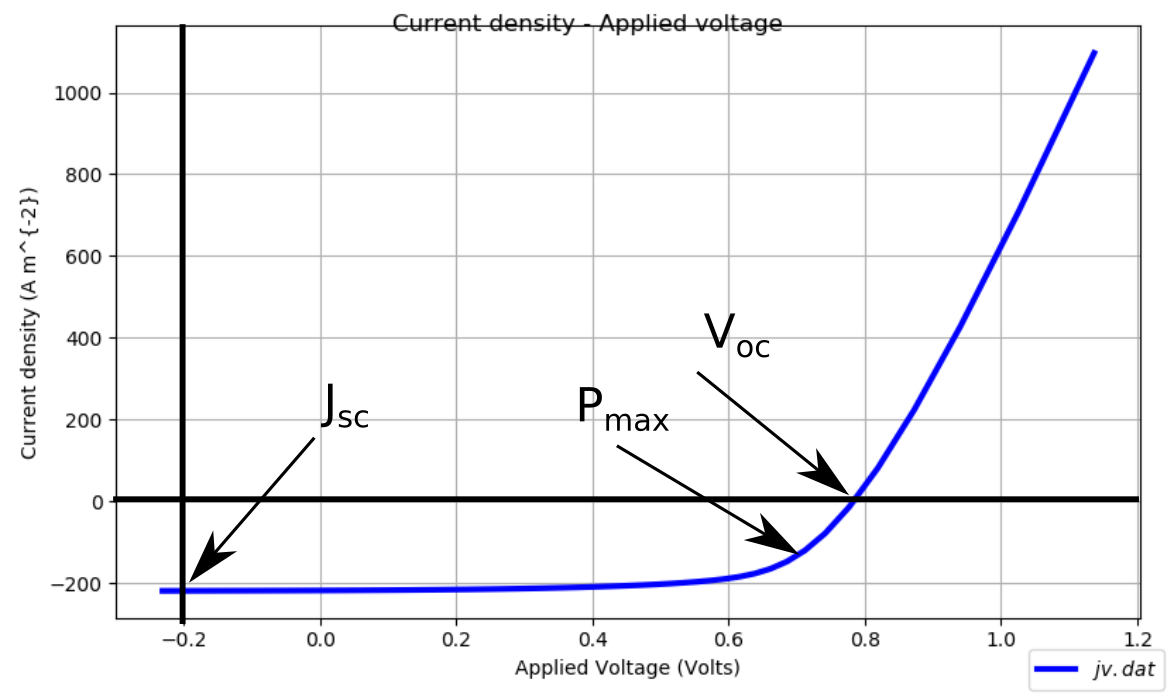
\includegraphics[width=0.6\textwidth]{./images/running/jv_curve.png}
\caption{The output tab}
\label{fig:jv_curve}
\end{figure}


Now try opening up the file $sim\_info.dat$, this file displays information on the performance of the solar cell, such as the Open Circuit Voltage ($V_{oc}$ - the maximum Voltage the solar cell can produce when iluminated), efficiency ($\eta$ - the efficiency of the cell) , and short circuit current ($J_{sc}$ - the maximum current the cell can produce when it is illuminated).  Figure \ref{fig:jv_curve}, shows where you can find these values on the JV curve.  The $sim\_info.dat$ file contains a lot of other parameters, these are described in detail in section \ref{sec:siminfo}.

\vspace*{\fill}
\fbox{
\parbox{0.9\textwidth}{
\color{blue} Question \addtocounter{question}{1}\thequestion: What is the $J_{sc}$, $V_{oc}$ and Fill Factor (FF) of this solar cell?  How do these number compare to a typical Silicon solar cell? (Use the internet to find typical values for a Silicon solar cell.)
}\par
}



\newpage
\subsection{Editing device layers}
\label{sec:layereditor}

\begin{minipage}{0.5\textwidth}
\centering
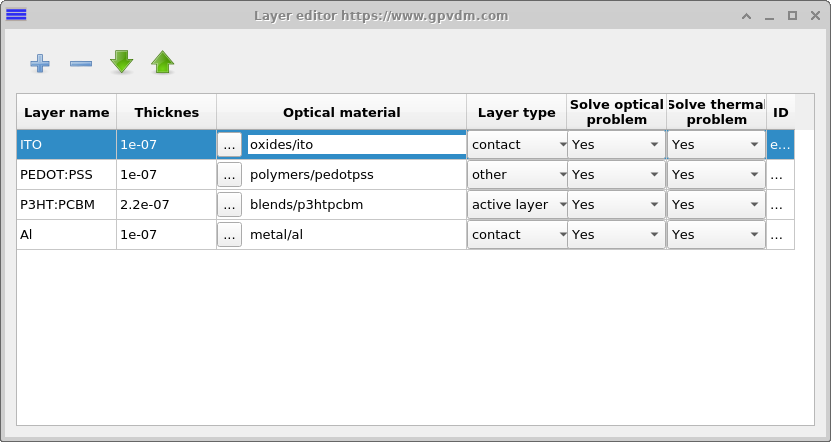
\includegraphics[width=\textwidth,height=0.7\textwidth]{./images/running/layer_editor.png}
\captionof{figure}{The layer editor window.}
\label{fig:layereditor}
\end{minipage}
\begin{minipage}[]{0.5\linewidth}
\hspace*{8px}
Any device in OghmaNano consists of a series of layers (this is sometimes referred to as the epitaxy - this is a term which comes from inorganic semiconductors). The layer editor can be accessed from the main simulation window, under the \emph{device structure} tab. This is visible towards the top of figure \ref{fig:simpleinterface}, and the layer editor is visible in figure \ref{fig:layereditor}. Within the window is a table that describes the structure of the device. The column thickness describes the thickness of each layer. The P3HT:PCBM layer is the layer of material which converts photons into electrons and holes, this is commonly called the active layer.
\end{minipage}
\vspace*{8px}
 An active layer thickness of 50nm is considered very thin for an organic solar cell, while an active layer of 400nm is considered very thick (too thick for efficient device operation). Vary the active layer between 50 nm and 400 nm, for each thickness record the device efficiency (I suggest you perform the simulation for at least eight active layer widths).



\subsubsection{More on the layer editor}
The layer editor has the following columns:

\begin{itemize}
  \item Layer name: Is the English name describing the layer. You can call your layers what you want (i.e. ITO, PEDOT, fred or bob) it has no physical meaning.
  \item Thickness: Is the layer thickness given in meters.
  \item Optical material: Specifies the n/k data which is used to describe the materials optical properties. In the simulation the n/k data are taken from experimental values stored in the optical database \ref{sec:materialdatabase} and have nothing to do with the electrical material properties such as effective band gap.
  \item Layer type: Specifies to the simulation how the layer is treated when performing a simulation. There are three types of layer
	\begin{itemize}
	  \item active: This type of layer is electrically active and the drift diffusion solver will solve the electrical equations in this layer type. See section \ref{sec:electrical}. You can have as many active layers as you like but they must be contiguous.
 	  \item contact: This tells the model that a layer is a contact and a voltage should be applied, see section \ref{sec:contacteditor} for more details.
 	  \item other: Any layer which is not a contact or active.

	\end{itemize}
\end{itemize}

%\vspace*{\fill}


\subsubsection{Which layers should be active?}
A common mistake people make when starting to simulate devices is to try to make all the layers in their device active because their logic is: Current must be flowing through them so they must be active right?  However, in for example a solar cell only the BHJ or in a perovskite device the perovskite layer will have both species of carriers (electrons+holes) and complex effects such as photogeneration, recombination and carrier trapping. So in this layer it makes sense to solver the drift diffusion equations.  Other layers which don't have both species of carriers can be treated simple parasitic resistances see section \ref{sec:parasitic}. I would only recommend setting other layers of the device to active (such as the HTL/ETL) if you are trying to investigate effects such as s-shaped JV curves or devices which clearly need multiple active layers such as OLEDs. In general, try to minimize the number of active layers and always keep simulations as simple as possible to explain the physical effects you see.  

\vspace*{\fill}
\fbox{
\parbox{0.9\textwidth}{
\color{blue} Task \addtocounter{question}{1}\thequestion : Plot a graph (using excel or any other graphing tool), of device efficiency v.s. thickness of the active layer. What is the optimum efficiency/thickness of the active layer? Also plot graph $V_{oc}$ , $J_{sc}$ and $FF$
as a function of active layer thickness. $J_{sc}$ is generally speaking the maximum current a solar cell can generate, try to explain your graph of J sc
v.s. thickness, [Hint, the next section may help you answer this part of the question.]
}\par
}




\newpage
\subsection{How do solar cells absorb light?}
In this section we are going to learn how a solar cells interact with light.  Firstly, let's have a look at the solar spectrum.  Sunlight contains many wavelengths of light, from ultraviolet light, though to visible light to infrared.  The human eye can only see a small fraction of the light emitted by the sun.  OghmaNano stores a copy of the suns spectrum to perform the simulations.  Let's have a look at this spectrum, to do this go to the \emph{Database} tab, the choose \emph{Optical database}.  This should, bring up a window as shown in figure \ref{fig:optical_database}

\begin{figure}[h!]
\centering
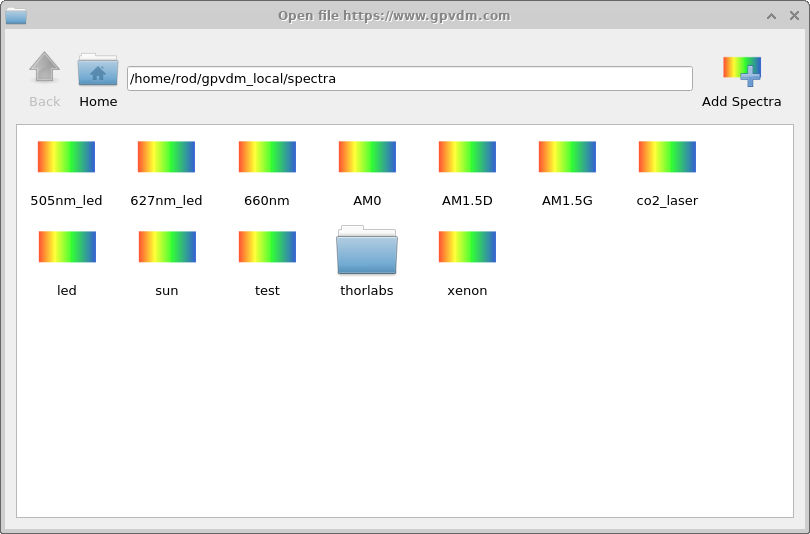
\includegraphics[width=0.6\textwidth]{./images/running/optical_database.png}
\caption{The optical database viewer}
\label{fig:optical_database}
\end{figure}

Double click on the icon called, \emph{AM1.5G}, this should bring up a spectrum of the sun's spectrum.  Have a look at where the peak of the spectrum is.  Now close this window, and open the spectrum called $led$.  Where is the peak of this spectrum.


\begin{figure}[H]
\centering
\begin{tabular}{ c c }

\raisebox{-.1\height}{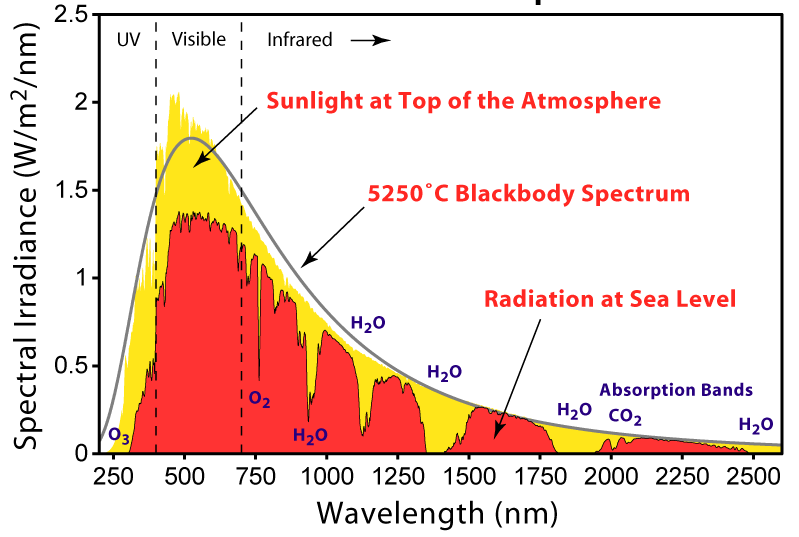
\includegraphics[width=0.45\textwidth]{./images/running/spectrum.png}}

&
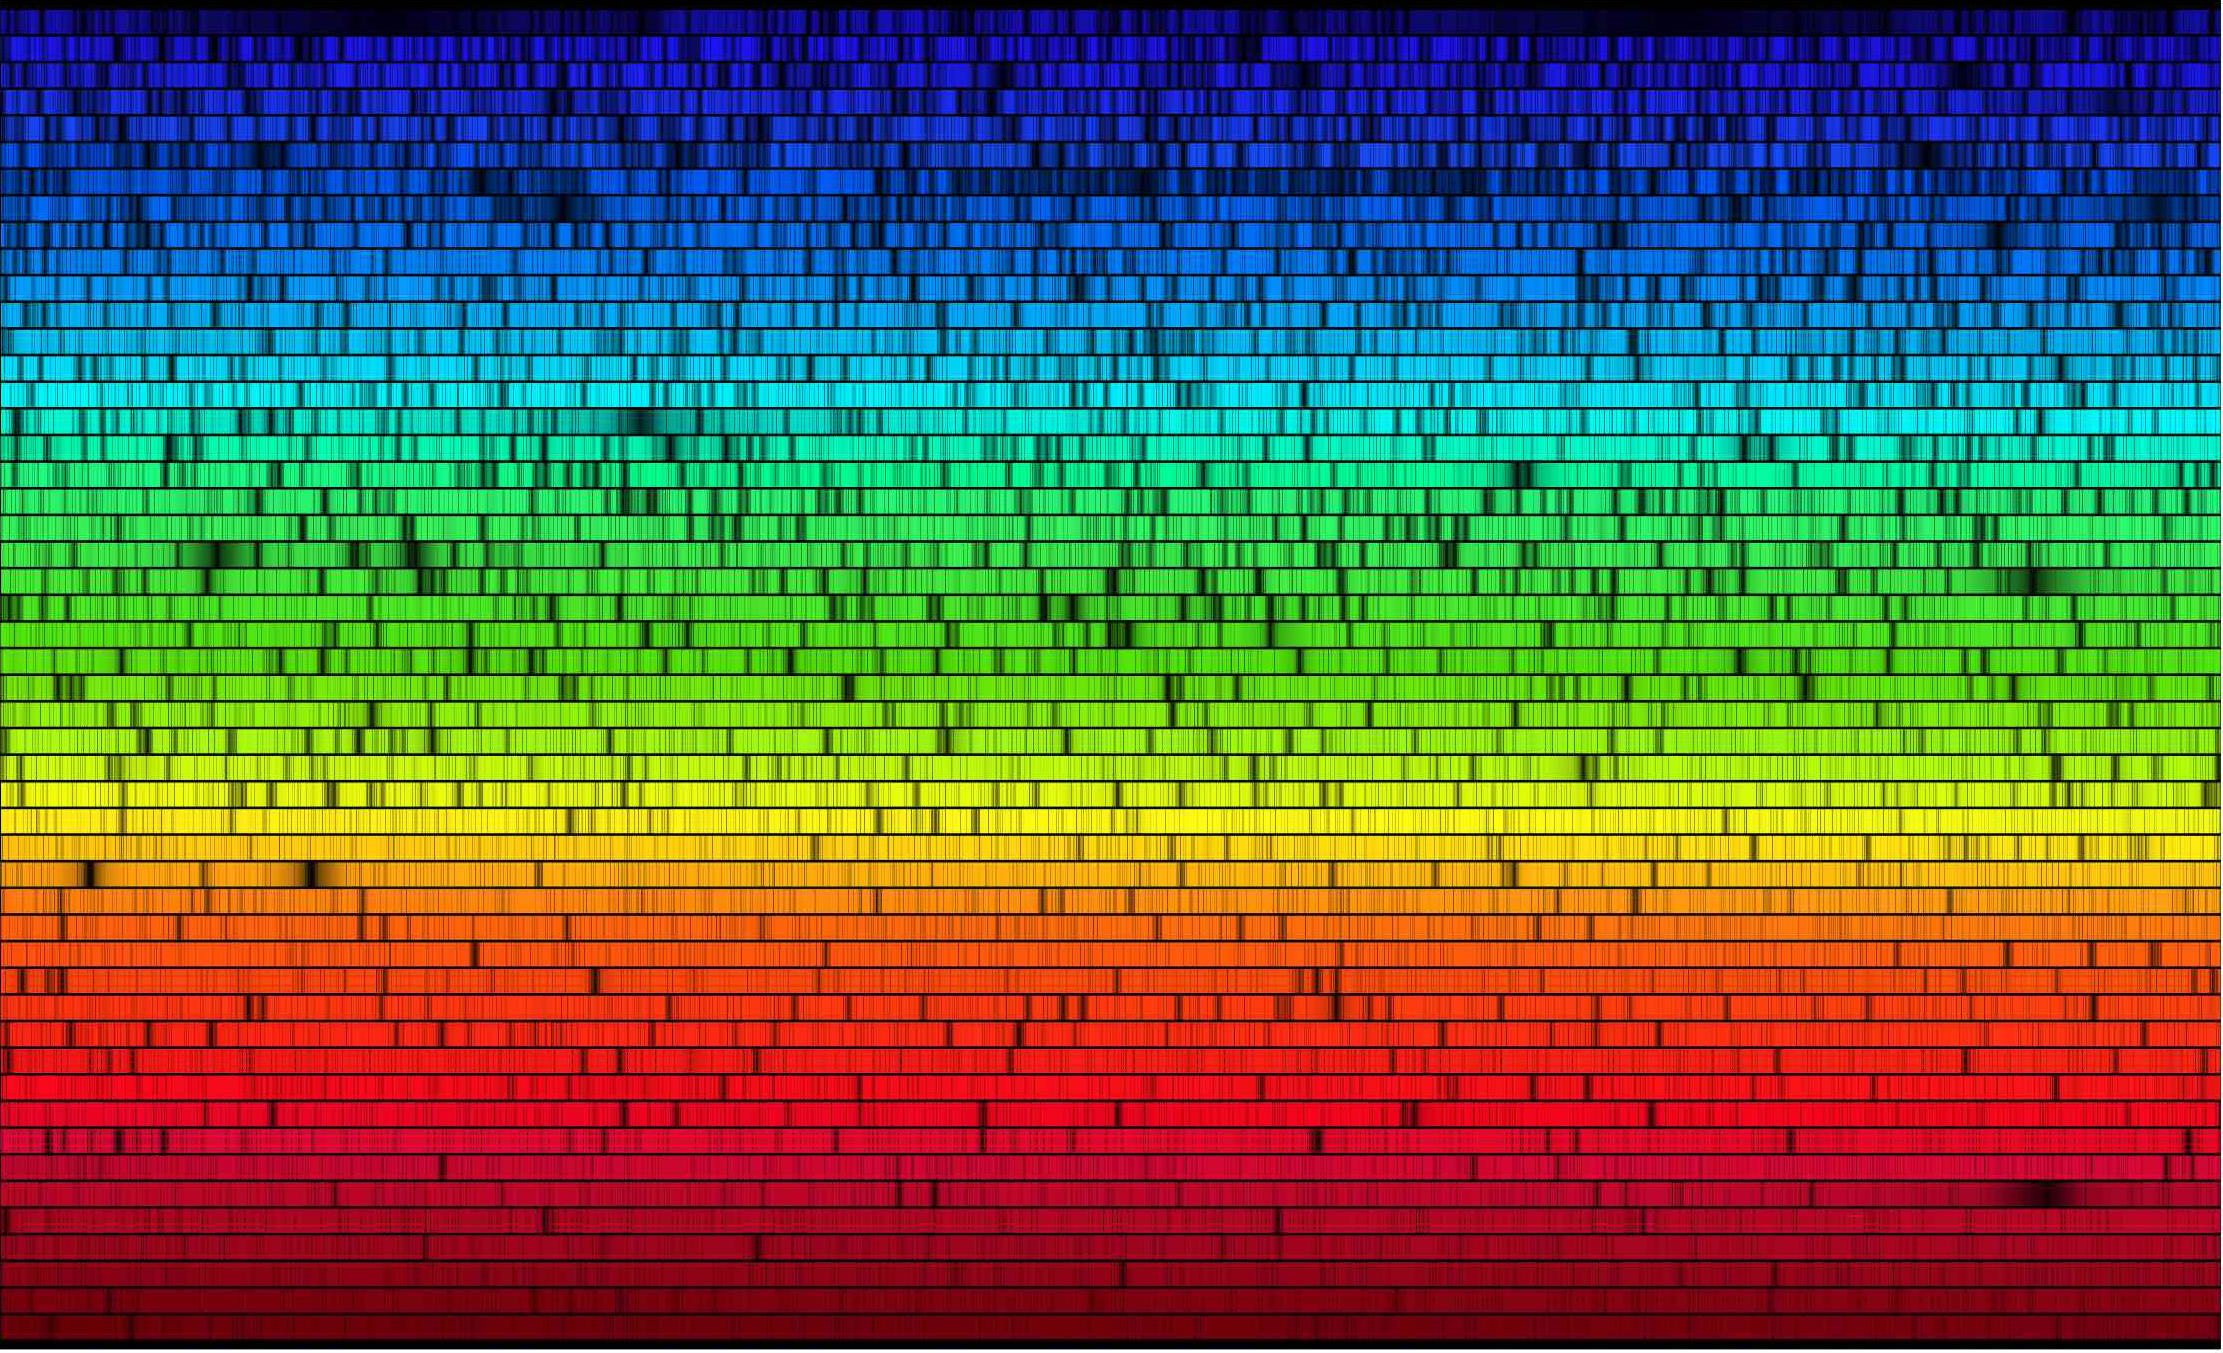
\includegraphics[width=0.45\textwidth]{./images/running/SolarCCD.jpg}
\\
\end{tabular}
\caption{a: A plot of the entire \href{https://commons.wikimedia.org/wiki/File:Solar_Spectrum.png}{solar spectrum}. b: The image below shows the \href{https://solarsystem.nasa.gov/resources/390/the-solar-spectrum/}{solar spectrum} at 392 nm (blue) to 692 nm (red) as observed with the Fourier Transform Spectrograph at Kitt Peak National Observatory in 1981. R. Kurucz }
\end{figure}


\vspace*{\fill}
\fbox{
\parbox{0.9\textwidth}{
\color{blue} Question \addtocounter{question}{1}\thequestion: Describe the main differences between the light which comes from the LED and the sun.  Rather than referring to the various regions of the spectrum by their wavelengths, refer to them using English words, such as $infrared$, $Ultra Violet$, $Red$, and $Green$ etc... you will find which wavelengths match to each color on the internet.  If you were designing a material for a solar cell, what wavelengths would.}
}

\newpage
\subsection{Light inside solar cells}
As you will have seen from when you fist opened the simulation, the solar cells are often made from many layers of different materials.  Some of these materials, are designed to absorb light, some are designed to conduct charge carriers out of the cell.  The simulator has a database of these materials, to look at the database, click on the $Database$ tab, the click on \emph{Material database}.  This should bring up a window as shown in figure \ref{fig:db}, once this is open navigate to the directory $polymers$, and double click on the material $p3ht$, in the new window click on the tab $Absorption$ (see figure \ref{fig:alpha}).  This plot shows how light is absorbed in the material as a function of wavelength.

\begin{figure}[h!]
\centering
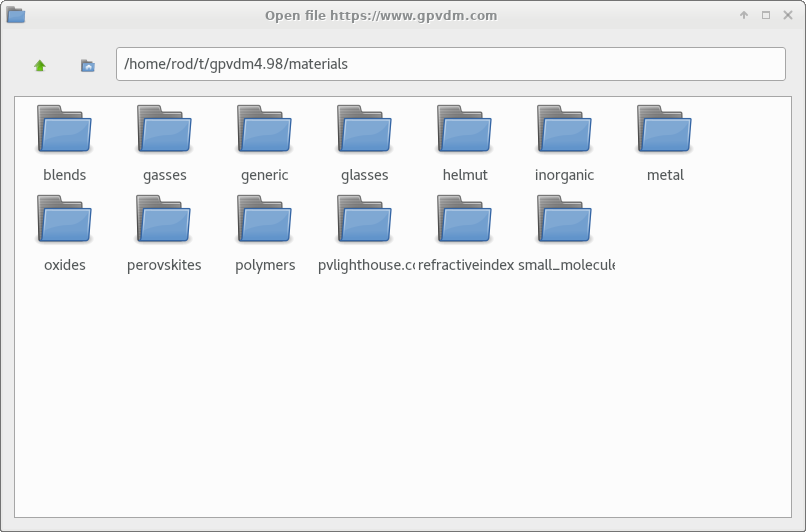
\includegraphics[width=100mm]{./images/running/db.png}
\caption{The materials database}
\label{fig:db}
\end{figure}

\begin{figure}[h!]
\centering
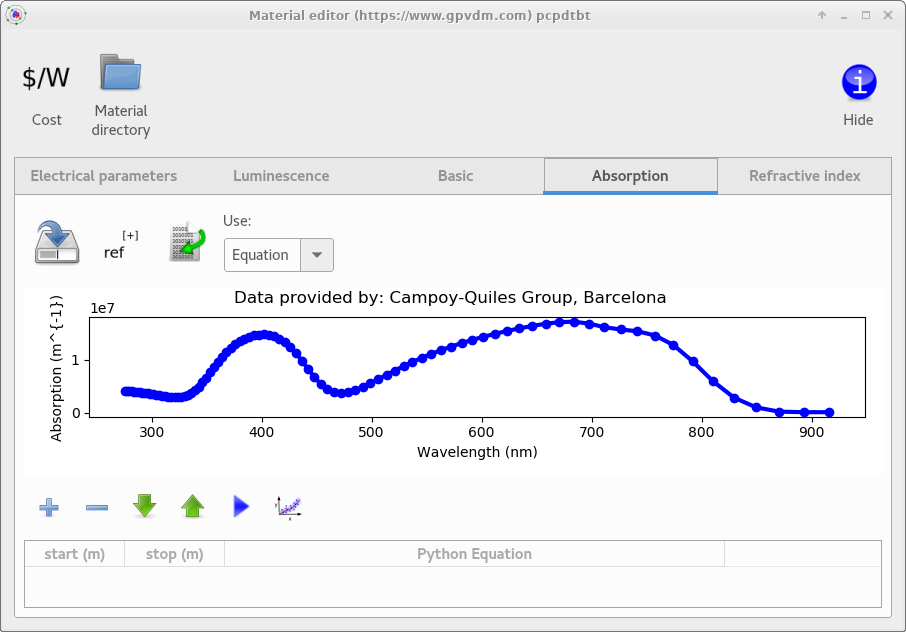
\includegraphics[width=100mm]{./images/running/alpha.png}
\caption{Optical absorption of the light.}
\label{fig:alpha}
\end{figure}

\vspace*{\fill}
\fbox{
\parbox{0.9\textwidth}{
\color{blue} Question \addtocounter{question}{1}\thequestion: What color of light does the polymer $p3ht$ absorb best?  Which material in the $polymers$ directory do you think will absorb the suns light best?}
}



\newpage
\subsection{Parasitic elements}
\label{sec:parasitic}

Many devices have parasitic shunt and series resistances associated with them.  Shunt resistances ($R_{s}$) are caused by conduction straight through the device in thin novel devices this is often caused by impurities in the material system.  Parasitic series resistances ($R_{s}$) are often associated with the resistance of the contacts, the resistance of the HTL/ETL or any other resistances which are not associated with the active layer.  These resistance can be seen for a typical solar cell in figure \ref{fig:parasitic_circuit} also shown in the figure is the ideal diode of the device. These resistances can be set in the parasitic component window shown in figure \ref{fig:parasitic}
\\
\\
\noindent
\begin{minipage}{0.45\textwidth}
\centering
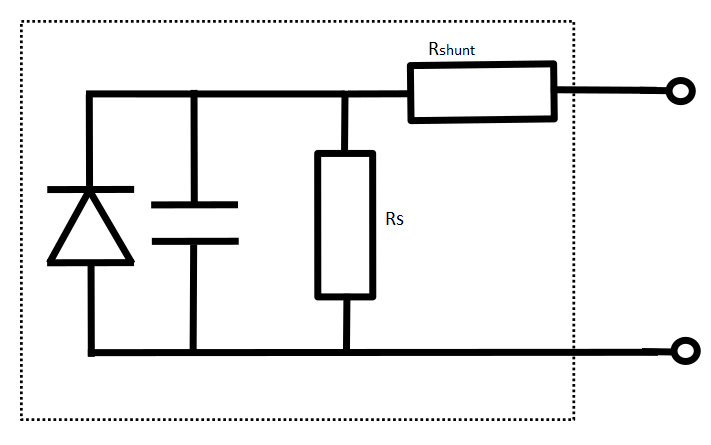
\includegraphics[width=\textwidth,height=0.7\textwidth]{./images/running/parasitic_circuit.png}
\captionof{figure}{Circuit model of a solar cell.}
\label{fig:parasitic_circuit}
\end{minipage}
\hspace*{10px}
\begin{minipage}[]{0.45\linewidth}
\centering
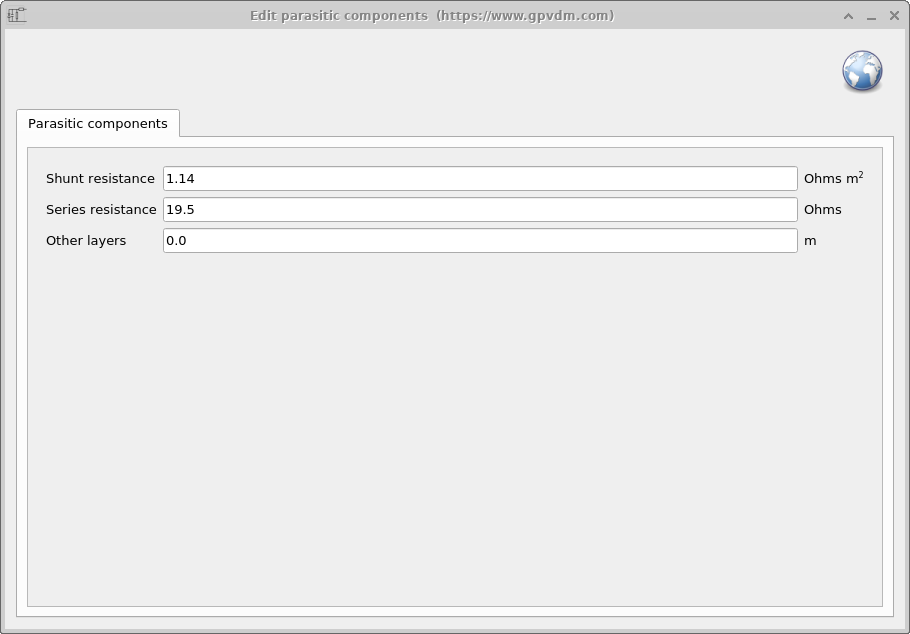
\includegraphics[width=\textwidth,height=0.7\textwidth]{./images/running/parasitic.png}
\captionof{figure}{The parasitic component editor.}
\label{fig:parasitic}
\end{minipage}


You can change the values of series and shunt resistance in OghmaNano, by going to the \emph{Electrical} tab and then clicking on the \emph{Parasitic components} button. Due to the flat broad contacts on a solar cell, there is often a capacitance associated with the device, this is important for transient measurements and can be calculated with the equation:

\begin{equation}
C=\frac{\epsilon_r \epsilon_0 A}{d+\Delta}
\end{equation}

where $A$ is the area of the device $\epsilon$ are the hyperactivities, and $d$ is the thickness of the device.  Often for various reasons the measured capacitance of the device does not match what one would expect from the above equation. Therefore the term "Other layers" ($\Delta$) has been added to the parasitic window to account for differences between measured capacitance and layer measured layer thicknesses.

\vspace*{\fill}
\fbox{
\parbox{0.9\textwidth}{
\color{blue} Task \addtocounter{question}{1}\thequestion : In the optical tab you will find a control called \emph{Light intensity}, this controls the amount of light which falls on the device in Suns.  Set it to zero so that the device is in the dark.  Then run two JV curve simulations, one with a shunt resistance of $1~Ohm~m^2$ and one with a shunt resistance of $1x10^{6}~Ohm~m^2$ (Hint you will have to enter $1e6$ in the text box).  What happens to the dark JV curve?  Now try running the same same simulations again but in the light.
}\par
}



\pagebreak
\subsection{Solar cells in the dark}
So far, all the simulations we have run have been performed in the light.  This is a logical, as usually we are interested in solar cell performance only in the light.  However, a lot of interesting information can be gained about solar cells by studying their performance in the dark.  We are now going to turn off the light in the simulation.  From the \emph{Optical} tab set the \emph{Light intensity (suns)} drop down menu to 0.0 Suns, this can be seen in figure \ref{fig:dark}.  The photons in the 3D image should disappear as seen in figure \ref{fig:dark}.
\\
\\
\begin{minipage}{0.45\textwidth}
\centering
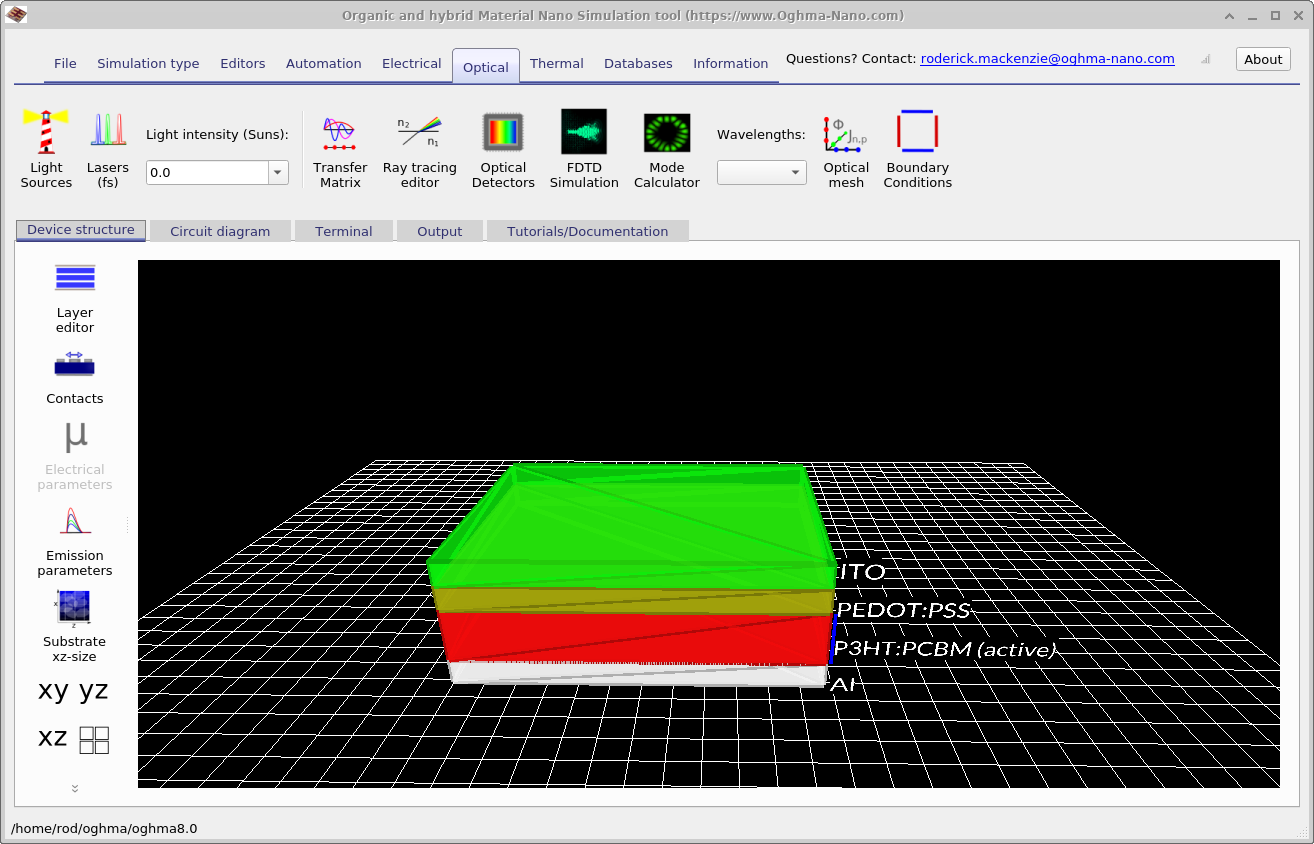
\includegraphics[width=\textwidth,height=0.7\textwidth]{./images/running/dark.png}
\captionof{figure}{Running OghmaNano in the dark, the Light intensity drop-down menu has been set to 0 Suns and the photons have disappeared from the image.}
\label{fig:dark}
\end{minipage}
\hspace*{10px}
\begin{minipage}[]{0.45\linewidth}
\centering
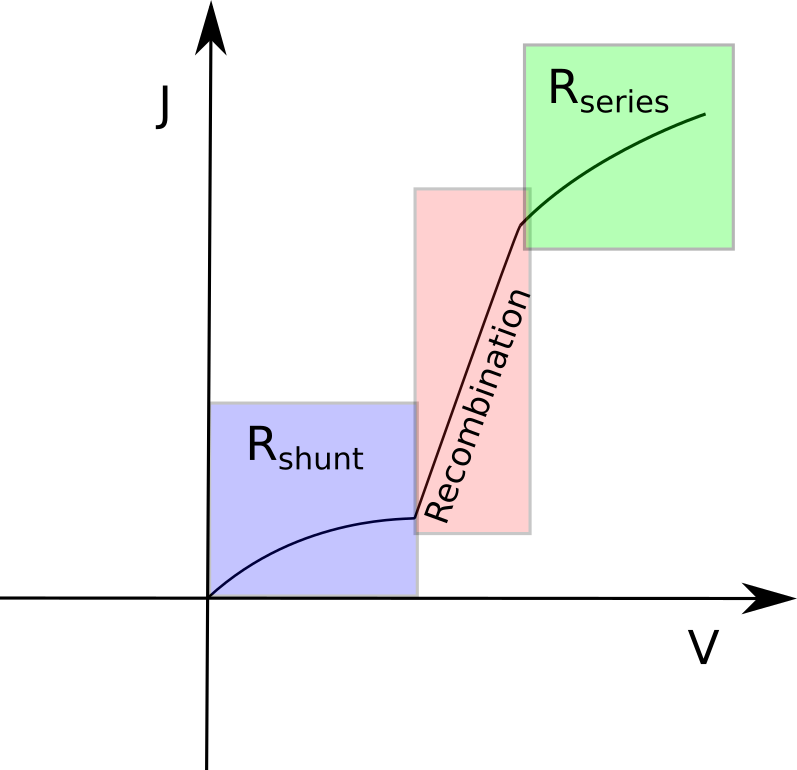
\includegraphics[width=\textwidth,height=0.7\textwidth]{./images/running/jv_dark.png}
\captionof{figure}{A sketch of a typical dark JV curve.}
\label{fig:jv_dark}
\end{minipage}
\\
\\
Now set the shunt resistance to $1M \Omega m^2$, and run a simulation.  Plot the jv curve.  It is customary to plot jv curves on a x-linear y-log scale.  To do this in the plot window, hit the 'l' key to do this.  The shape should resemble, the JV curve in figure \ref{fig:jv_dark}.  Certain solar cell parameters affect different parts of the dark JV curve differently, the lower region is affected very strongly by shunt resistance, the middle part is affected strongly by recombination, and the upper part is strongly affected by the series resistance.

\vspace*{\fill}
\fbox{
\parbox{0.9\textwidth}{
\color{blue} Question \addtocounter{question}{1}\thequestion: What values of series and shunt resistance, would produce the best possible solar cell?  Enter these values into the device simulator and copy and paste the dark JV curve into your report.
}\par
}



\newpage
\subsection{The contact editor}
\label{sec:contacteditor}
The contact editor is used to configure the electrical contacts.  Which layers act as contacts is configured in the layer editor see section \ref{sec:layereditor}.  The contact editor has the following fields:

\begin{figure}[H]
\centering
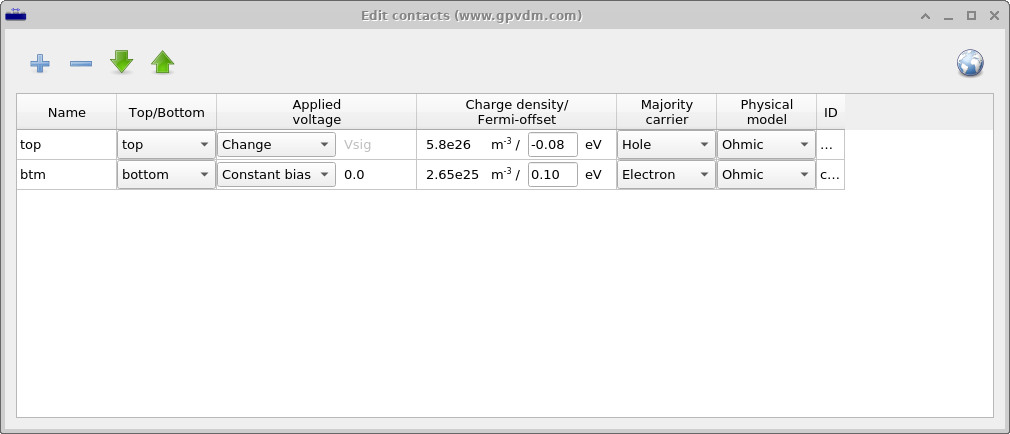
\includegraphics[width=0.5\textwidth,height=0.3\textwidth]{./images/running/contact_editor.png}
\caption{The contact editor}
\label{fig:contacteditor}
\end{figure}

\begin{itemize}
  \item Name: The name of the contact, this can be any English word. It has no physical meaning.
  \item Top/Bottom: Sets if the contact is on the top, bottom or in 2D simulation left and right of the device are also valid.
  \item Applied voltage: Sets the applied voltage on the contact. You first have to select what type of applied voltage you want:
		\begin{itemize}
		\item Ground: This will set the contact to zero volts i.e. ground. 0V is always taken as ground.
		\item Constant bias: This will apply a constant bias to a contact.  It can be set to zero, and would then be equivalent to ground.  In OFET simulations the voltage value can be set to bias one contact to a desired constant voltage.
		\item Change: If a contact is set to 'Change' this tells the simulation to apply a changing voltage to this contact. For example if you are performing a JV sweep, the sweep voltage will be applied to this contact.  Similarly if you are doing an IS simulation (TPV, TPC, ToF etc..) the voltage will be applied/measured to this contact.
		\end{itemize}
  \item Charge density: This sets the majority charge density on the contacts. The Fermi-offset is calculated from the charge density. The model does not use Fermi-offset as an input, it uses charge density.
  \item Majority carrier: This sets the majority carrier density to electrons or holes.
  \item Physical model: This selects if you have ohmic contacts or schottky contacts. I recommend using ohmic contacts.

\end{itemize}

\vspace*{\fill}

\fbox{
\parbox{0.9\textwidth}{
\color{blue} Task \addtocounter{question}{1}\thequestion : For a good contact which results in a high efficiency device, the Fermi-offset will be exactly 0 eV or very small. Firstly set the Fermi-offset to zero for both contacts, and run a simulation.  What efficiency cell do you get? Now set the Fermi-offset to $0.3 eV$ what efficiency cell do you now have? Make a note of the charge densities on the contacts which these Fermi-offsets produce. 
}\par
}



\newpage
\subsection{Electrical parameters}
\label{sec:doseditor}
The electrical parameter editor enables you to change the electrical parameters associated with the active layers. Here you can change mobilities, trap constants etc. If you set a layer to active wihtin the layer editor it will apear within the electrical paramter editor. The toolbar at the top of the window allows you to turn off and on various electrical mechanisms including:

\begin{itemize}
  \item Drift diffusion: This enabled drift diffusion within the layer. In most circumstances if a layer is set to be active there is no reason why you would want to turn this option off. The one example is in the insulating layer of an OFET.
  \item Auger recombination: This switches on and off Auger recombination. See \ref{sec:auger} for more information.
  \item Dynamic SRH traps: This is used to turn on and off dynamic SRH traps.  See section \ref{sec:SRHintro} for more information. This option should be turned on when modeling disordered semiconductors such as organic materials.
  \item Equilibrium SRH traps: This can be used to introduce a single equilibrium trap level.  See section \ref{sec:SRHintro} for more information.
  \item Excitons: This enables the exciton diffusion equation to be solved along with the electrical equations. See section \ref{sec:excitions} for more information.
  \item Excitons: This enables singlet and triplet states to be modelled.
\end{itemize}

\begin{figure}[H]
\centering
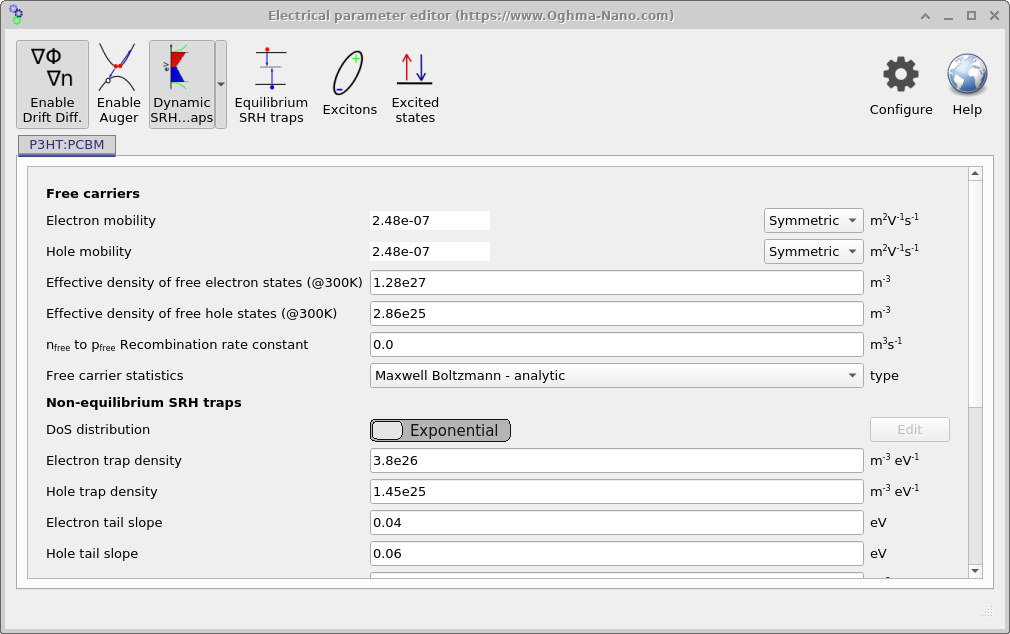
\includegraphics[width=100mm,height=70mm]{./images/running/dos_editor.png}
\caption{Electrical parameter window}
\label{fig:electricalparamwindow}
\end{figure}

\vspace*{\fill}
\fbox{
\parbox{0.9\textwidth}{
\color{blue} Task \addtocounter{question}{1}\thequestion : The values of electron mobility dictate how easily charge can move in the device.  You can think of this value as akin to resistance or a sort of microscopic resistance. Try try increasing the mobilities by two orders of magnitude and look what happens to the light JV curve of the device and the efficiency, FF, $V_{oc}$ and $J_{sc}$  Do you think it is good to have a low or high value of mobility?
}\par
}


\newpage
\fbox{
\parbox{0.9\textwidth}{
\color{blue} Task \addtocounter{question}{1}\thequestion : Recombination is described later in detail but for now we can simply think of it as how many electrons and holes meet each other in a given time. As stated above there are various types of recombination which can happen in organic semiconductors, but for now we will \emph{just consider}  the case when a free electron meets a free hole.  This is sometimes called bi-molecular recombination, the equation for this is given by:
\begin{equation}
R(x)=kn(x)p(x)
\end{equation}
Where $n(x)$ is the density of electrons and $p(x)$ is the density of holes, and k is a rate constant.  Before trying to understand this rate, firstly turn off the more complex SRH recombination by clicking on the \emph{Dynamic SRH traps} in figure \ref{fig:electricalparamwindow}.  You will notice lots of text boxes disappear. Then try changing the value of $k$ which is set in the text box called $n_{free}$ to $p_{free}$ Recombination rate constant, from 1e-15 to 1e-20 in five steps.  Run a simulation each time you change the value and make a graph of the efficiency of the cell as you change the value. 
}\par
}

\subsubsection{How do I know what electrical parameters to use?}
For traditional semiconductors that have been studied for years such as AlGaAs or InP the values of charge carrier mobility, band gap, electron  affinity (etc..) are well known and can simply be looked up on sites such as \href{https://www.ioffe.ru/SVA/NSM/Semicond/AlGaAs/index.html}{this} or in books such in Piprek's \cite{piprek2013semiconductor} excellent book. These materials are highly pure (99.999999999\%) (the so-called "eleven nines" purity). This means that when one has a sample of such a semiconductor one knows exactly what one has in the hand and what its physical properties will be. Organic semiconductors (also other novel materials such as perovskites etc..) on the are typically only 99.9\% on a good day, that is a whole eight orders of magnitude less pure than their traditional counterparts. This means that when one has a sample of such a material one is not exactly sure what material one has hold of so it's harder to know what the values of mobility etc will be.

Furthermore, traditional semiconductors are very ordered, this means that the atoms within them pack in a regular lattice (think marbles packing in a biscuit tin) this again helps make their electronic properties predictable. Novel semiconductors on the other hand are typically much more disordered than their traditional counterparts and consist of a higgldy piggidly collection of polymers/molecules (or perovskite domains etc..), and the exact structure of these materials depends very much on how they were deposited. This means that due to fabrication techniques/conditions varying between different labs, nominally the same material produced by the same suppler but can behave very differently depending on when/who/where it was deposited by.

So this brings us back to the question that started this section, what parameters should I use for my novel device? Here are some tips:

\begin{itemize}
  \item Use the base simulations provided in OghmaNano, these simulations have either been calibrated against real experimental devices or use very reasonable electrical parameters.
  \item Look in the literature and try to get an idea of what values are sensible ranges for the material systems you are looking at.
  \item Find some experimental data and make sure the current voltage curves produced by the model are within the same ball park as what you would expect experimentally, if they are totally out then you might need to tweak your electrical paramters.
  \item Fit the model to an experimental data set as was done in \cite{mackenzie2012extracting} and described in section \ref{sec:fitting} (This is however quite a hard thing to do though and not really recommended).
\end{itemize}



\chapter{Simulation modes and simulation editors}
\label{sec:simmodes}

OghmaNano uses a modular architecture that enables the core solver to perform a variety of simulation types using \index{plugins}. For example there is a plugin to perform steady state JV simulations, another plugin to perform frequency domain simulations, and another to calculate the Quantum Efficiency. They all leverage the same OghmaNano core solver but run it in a slightly different way with custom inputs and outputs. A list of the plugins and what they do can be found below:

\begin{itemize}
	\vspace{-0.2cm}\item Plugins for various types of experiment
	\begin{itemize}
		\vspace{-0.2cm}\item jv: To calculate steady state JV curves.
		\vspace{-0.2cm}\item suns\_jsc: Simulate suns v.s. Jsc curves.
		\vspace{-0.2cm}\item suns\_voc: Suns v.s. Voc simulations.
		\vspace{-0.2cm}\item eqe: Simulates EQE.
		\vspace{-0.2cm}\item cv: Capacitance voltage simulations.
		\vspace{-0.2cm}\item ce: To simulate charge extraction experiments.
		\vspace{-0.2cm}\item time\_domain: A time domain solver for transient simulations.
		\vspace{-0.2cm}\item fx\_domain: Simulate the frequency domain response of a device, both electrical and optical excitation.
		\vspace{-0.2cm}\item pl\_ss: Calculate the PL spectrum at in steady state.
		\vspace{-0.2cm}\item mode: Used to solve optical modes in 1/2D waveguides.
		\vspace{-0.2cm}\item spm: Simulates scanning probe microscopy in 3D electrical simulations.
		\vspace{-0.2cm}\item equilibrium: Equilibrium electrical simulations.
		\vspace{-0.2cm}\item exciton: Exciton simulations.
		\vspace{-0.2cm}\item mesh\_gen: Generates meshes.
	\end{itemize}
	\vspace{-0.2cm}\item Optical solver plugins
	\begin{itemize}
		\vspace{-0.2cm}\item fdtd: Finite Difference Time Domain (FDTD) optical solver.
		\vspace{-0.2cm}\item optics: Optical transfer matrix solver for 1D structures
		\vspace{-0.2cm}\item light\_full: Optical transfer matrix solver.
		\vspace{-0.2cm}\item light\_qe: Calculates optical profile using the experimental quantum efficiency.
		\vspace{-0.2cm}\item light\_exp: Calculates optical profile assuming exponential propagation of light in 1D structures.
		\vspace{-0.2cm}\item light\_flat: Calculates optical profile assuming flat optical profiles in the structure.
		\vspace{-0.2cm}\item light\_constant: Assumes user given values of generation rate in optical structures.
		\vspace{-0.2cm}\item light\_fromfile: Takes a generation rate from a file.
	\end{itemize}
\end{itemize}

In the simulation editors ribbon (see Figure \ref{fig:simeditors}) you can see icons that represent each plugin, these are the simulation editors. By clicking on an icon in this ribbon you will be able to edit how the plugin performs the various simulations.  For example in the JV simulation editor one can change the start/stop voltages of a voltage sweep.  The JV editor can be seen in Figure \ref{fig:jv_low}. Within each simulation editor the user can define multiple so called \emph{experiments}. This can be seen in below in Figure \ref{fig:jv_low} and Figure \ref{fig:jv_high}, where two JV scans have been defined within the JV editor, one called \emph{JV curve - low voltage} and another called \emph{JV curve - high voltage}. One has a start voltage of 0.02V and stop voltage of 1.0V, while the other has a start voltage of 1.0V and a stop voltage of 10V.  This feature is most useful in more complex experiments such as in time domain experiments where one may want to simulate multiple different voltage/light ramps/pulses for one device. There is no limit to how many \emph{experiments} can be defined for each plugin.
\\
\begin{figure}
\centering
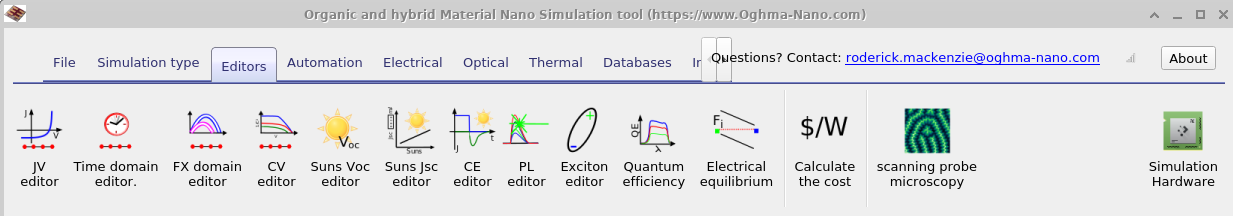
\includegraphics[width=\linewidth,height=0.2\linewidth]{./images/sim_editors/ribbon_sim_editors.png}
\caption{Simulation editors use this toolbar to edit the various simulation conditions your device will experience.}
\label{fig:simeditors}
\end{figure}

\begin{minipage}{0.5\textwidth}
	\centering
	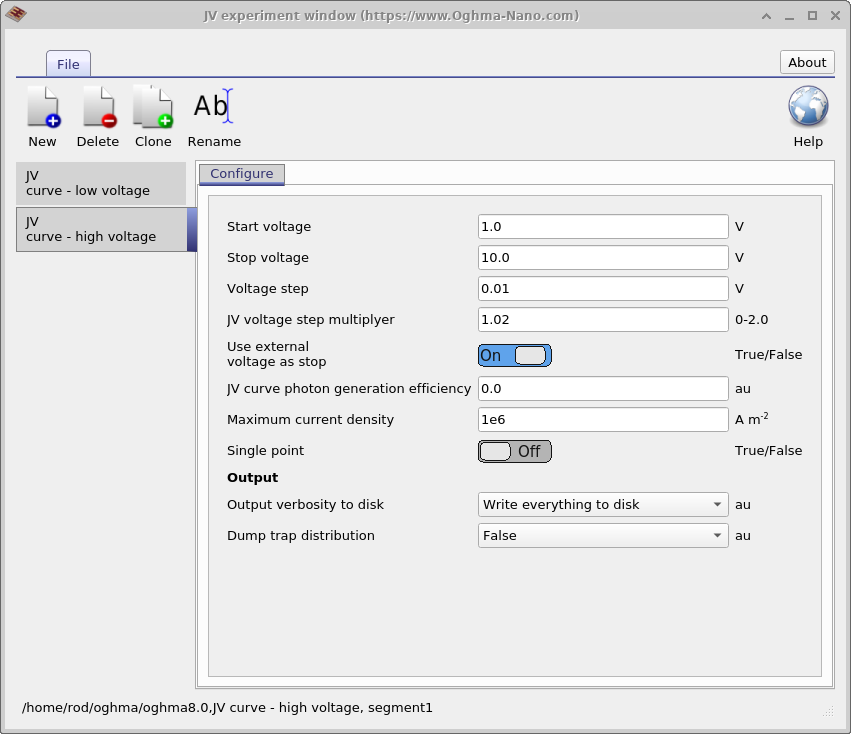
\includegraphics[width=\linewidth,height=0.8\linewidth]{./images/sim_editors/jv_high_voltage.png}
	\captionof{figure}{An experiment set up in the JV window for high voltage simulations.}
	\label{fig:jv_low}
\end{minipage}
\hspace{4pt}
\begin{minipage}[]{0.5\linewidth}
	\centering
	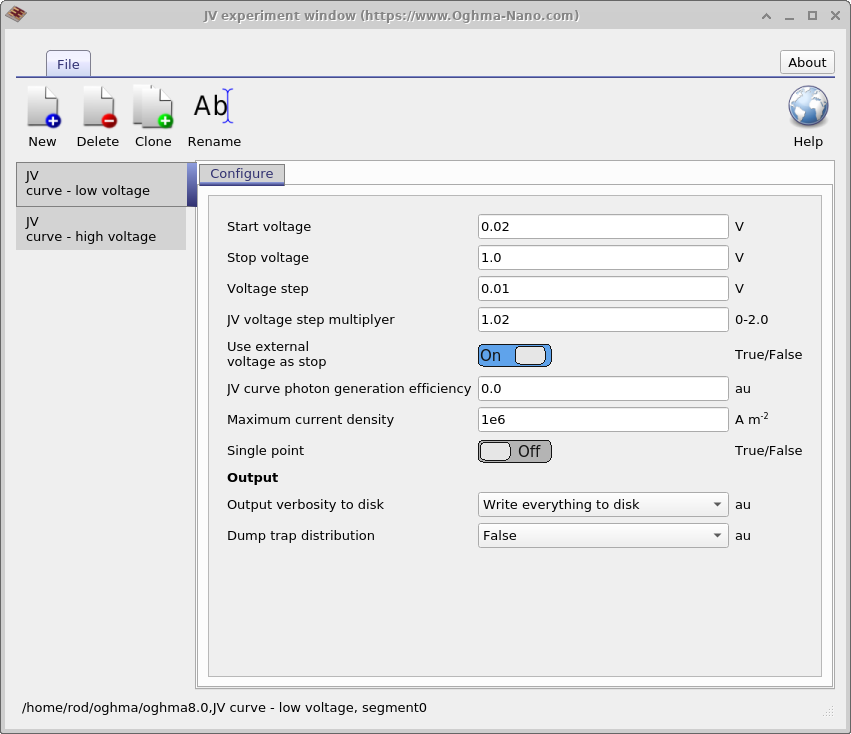
\includegraphics[width=\linewidth,height=0.8\linewidth]{./images/sim_editors/jv_low_voltage.png}
	\captionof{figure}{An experiment set up in the JV window for low voltage simulations.}
	\label{fig:jv_high}
\end{minipage}

Once an \emph{experiment} has been defined an icon representing it will appear in the simulation mode ribbon shown in figure \ref{fig:simmodes}. You can see in the figure an icon for \emph{JV curve low voltage} and \emph{JV curve high voltage} that were defined in Figure \ref{fig:jv_low} and \ref{fig:jv_high}. You can see in Figure \ref{fig:simmodes} that \emph{JV curve low voltage} is depressed. This means that when the simulation is run this simulation mode will be executed. If you select another simulation mode, then when the play button (or F9) is pressed that simulation mode will be run. Only one simulation mode can be run at a time.


\begin{figure}[H]
\centering
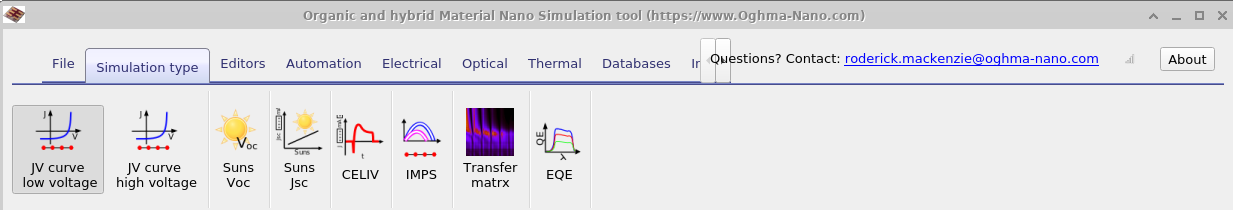
\includegraphics[width=\linewidth,height=0.2\linewidth]{./images/sim_editors/ribbon_sim_modes.png}
\caption{Selecting a simulation mode, in this case the \emph{JV curve low voltage} has been selected so that when the user presses play that simulation mode will be run.}
\label{fig:simmodes}
\end{figure}

\newpage
\section{JV editor (Steady state simulation editor)}
If you click on the JV editor icon in figure \ref{fig:ribbon_jv}, the JV editor window will open shown below in figure \ref{fig:jvcurveeditor}.

\begin{figure}[H]
\centering
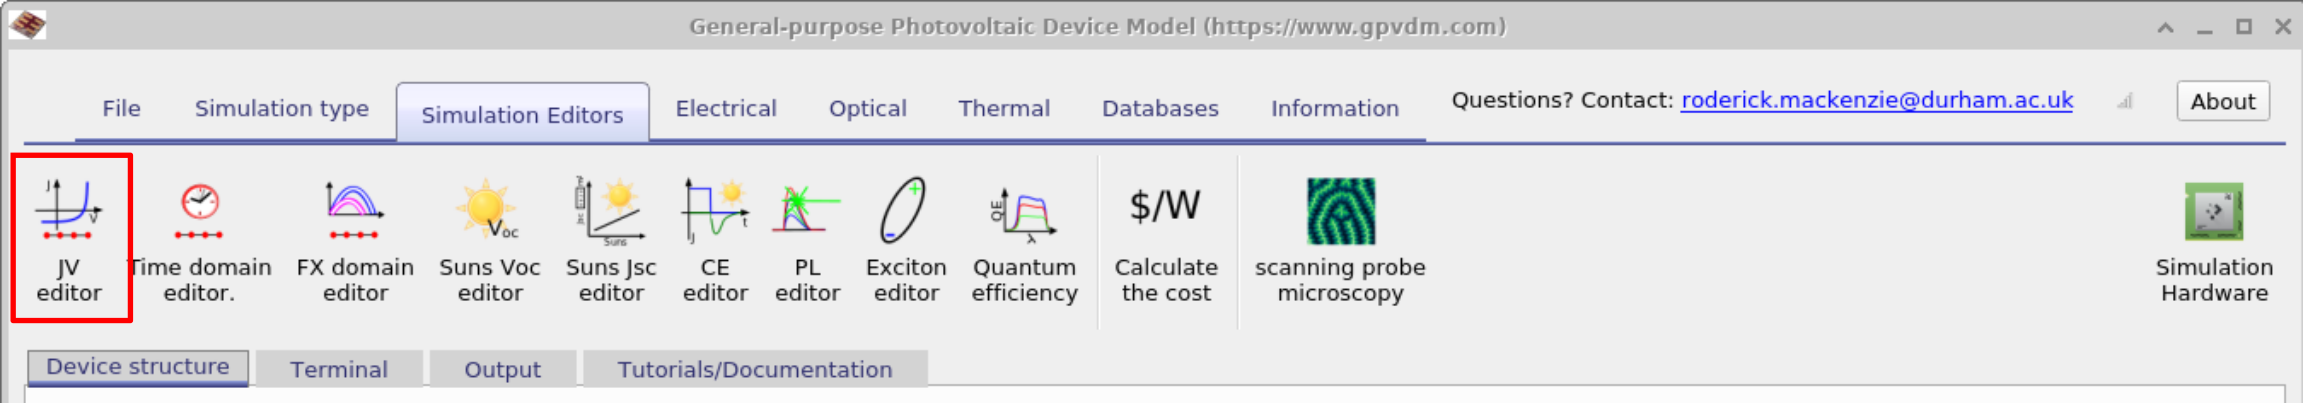
\includegraphics[width=0.8\textwidth]{./images/sim_editors/ribbon_jv.png}
\caption{Opening the JV editor from the simulation editor ribbon.}
\label{fig:ribbon_jv}
\end{figure}

This window can be used to configure steady state simulations. It does not matter if you are running a current-voltage sweep on a solar cell or an OFET.  This plugin will steadily ramp the voltage from a start voltage to a stop voltage.  The voltage will be applied to the \emph{active} contact as defined in the \emph{contact editor}.  You can set the start voltage, stop voltage and step size.  Use \emph{JV voltage step multiplayer} to make the voltage step grow each step.  The default is 1.0, i.e. no growth.

\begin{figure}[H]
\centering
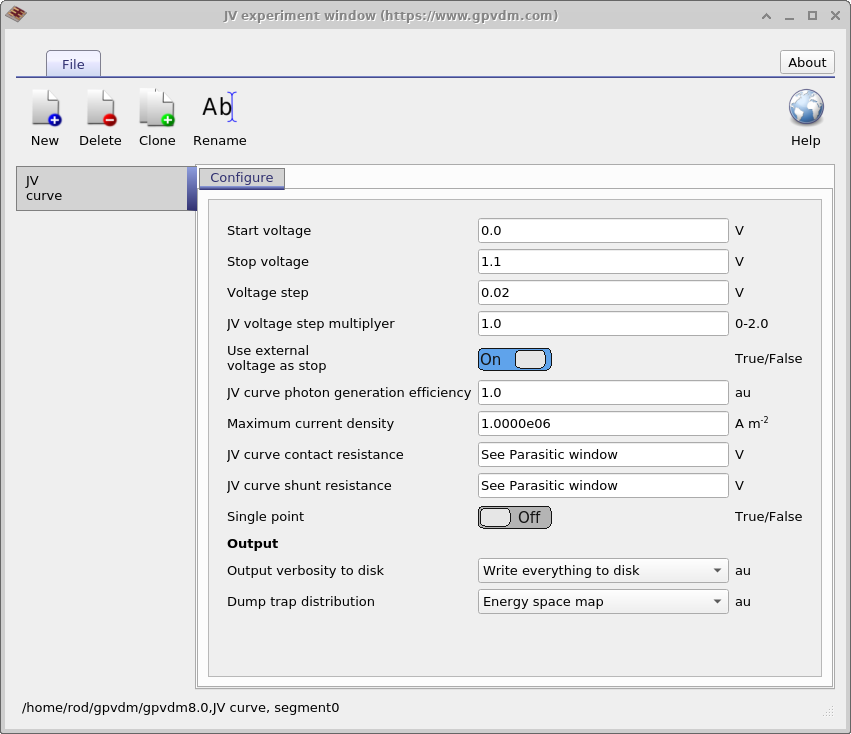
\includegraphics[width=0.7\textwidth,height=0.6\textwidth]{./images/sim_editors/jv_editor.png}
\caption{The JV editor editor window, use this to configure steady state simulations.}
\label{fig:jvcurveeditor}
\end{figure}

The files produced by the JV simulation mode are given in table \ref{tab:jv_output}.

\begin{table}[H]
\begin{center}
\begin{tabular}{ |c|c|c| } 
 \hline
	File name 			& 	Description  \\ 
 \hline
	$jv.dat$ 			&	Current voltage curve \\ 
	$charge.dat$ 		&	voltage charge density\\ 
	$k.csv$ 			&	Recombination constant k\\ 
	$sim\_info.dat$ 	&	Calculated $V_{oc}$, $J_{sc}$ etc.. see \ref{sec:siminfo}   \\

 \hline
\end{tabular}
\caption{Files produced by the JV simulation}
\label{tab:jv_output}
\end{center}
\end{table}



\newpage
\section{Time domain editor}
Related YouTube videos:
\begin{figure}[H]

\begin{tabular}{ c l }


\includegraphics[width=0.05\textwidth]{./images/youtube.png}

&
\href{https://www.youtube.com/watch?v=D7yJLFmTAVQ}{Simulating optoelectronic sensors made from polymers.}

\end{tabular}
\end{figure}

The time domain editor can be used to configure time domain simulations, this is shown in figure \ref{fig:timedomaineditor}.  You can see that one simulation editor can be used to edit multiple simulations.  The panel on the left shows the editor being used to edit a CELIV simulation while the panel on the right shows the editor being used to edit a TPC simulation.  The new, delete and clone buttons in the top of the window can be used to make new simulation modes. The table in the bottom of the window can be used to setup the time domain mesh, apply voltages or light pulses.

\begin{figure}[H]
\centering
\begin{tabular}{ c c }

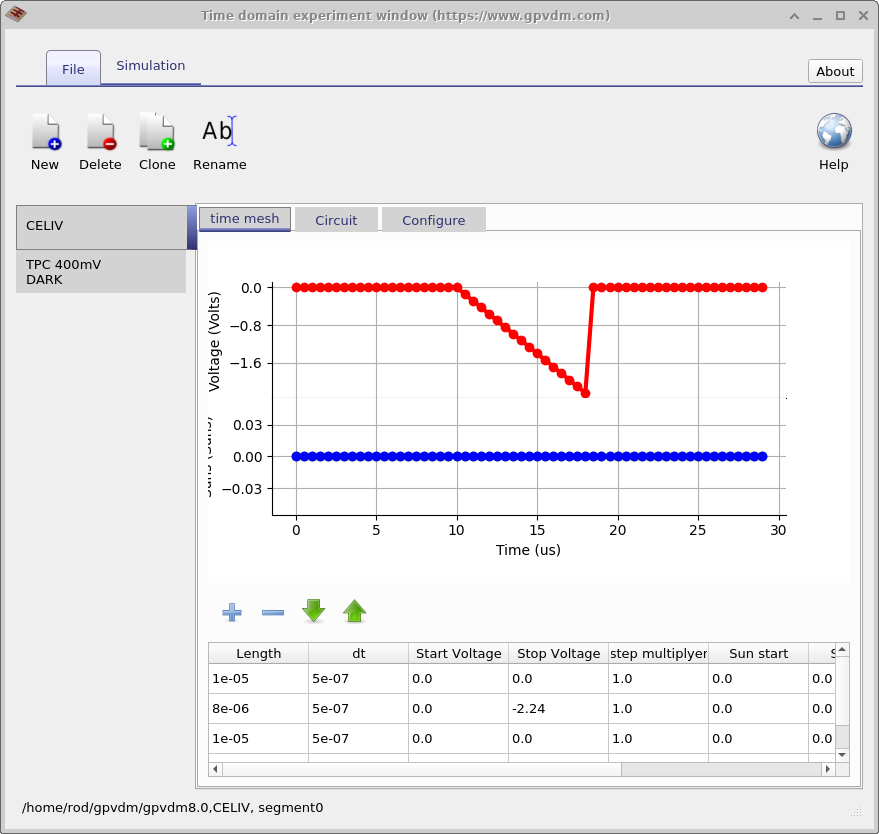
\includegraphics[width=0.5\textwidth,height=0.4\textwidth]{./images/time_domain_editor.png}

&
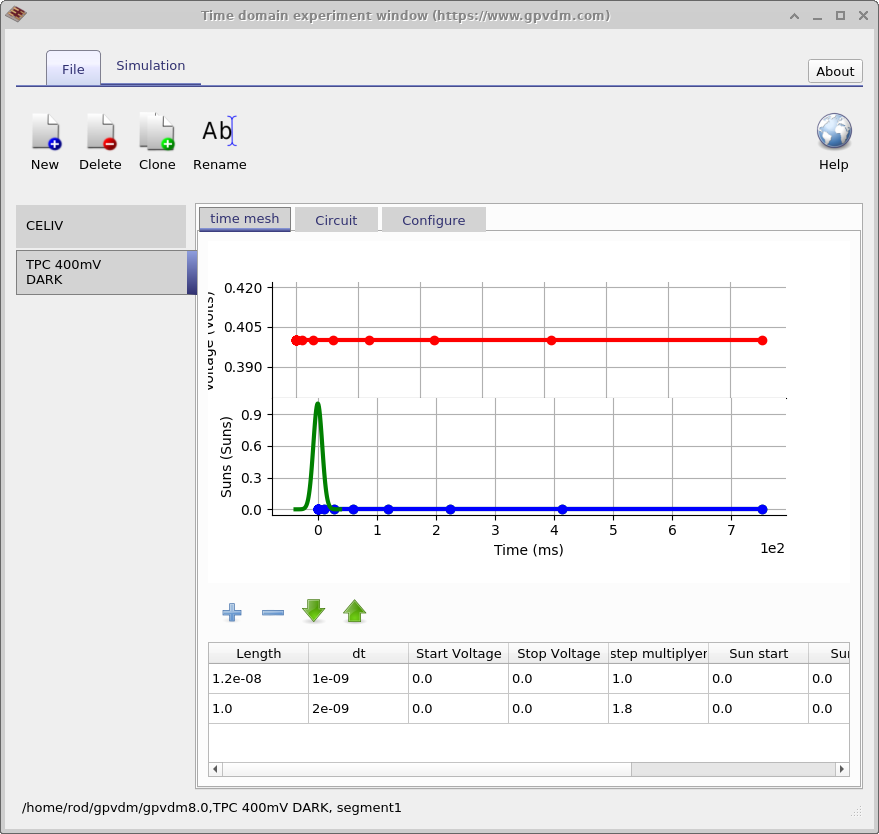
\includegraphics[width=0.5\textwidth,height=0.4\textwidth]{./images/time_domain_editor2.png}

\\

\end{tabular}
\caption{The time domain editor showing the user editing the duration of light/voltage pulses.}
\label{fig:timedomaineditor}
\end{figure}

Figure \ref{fig:timedomaineditor2} shows different tabs in of the time domain editor. The image on the left shows the circuit diagram used to model the CELIV experiment. From the left of the image the diode on the left accounts for the drift diffusion simulations it is in effect a perfect diode.  Then comes a capacitor used to model the charge on the plates of the device, then a shunt resistance and then the series resistance.  The final resistor on the right represents the external resistance of the measuring equipment.  The right hand figure shows the configuration options of the time domain window.

\begin{figure}[H]
\centering
\begin{tabular}{ c c }

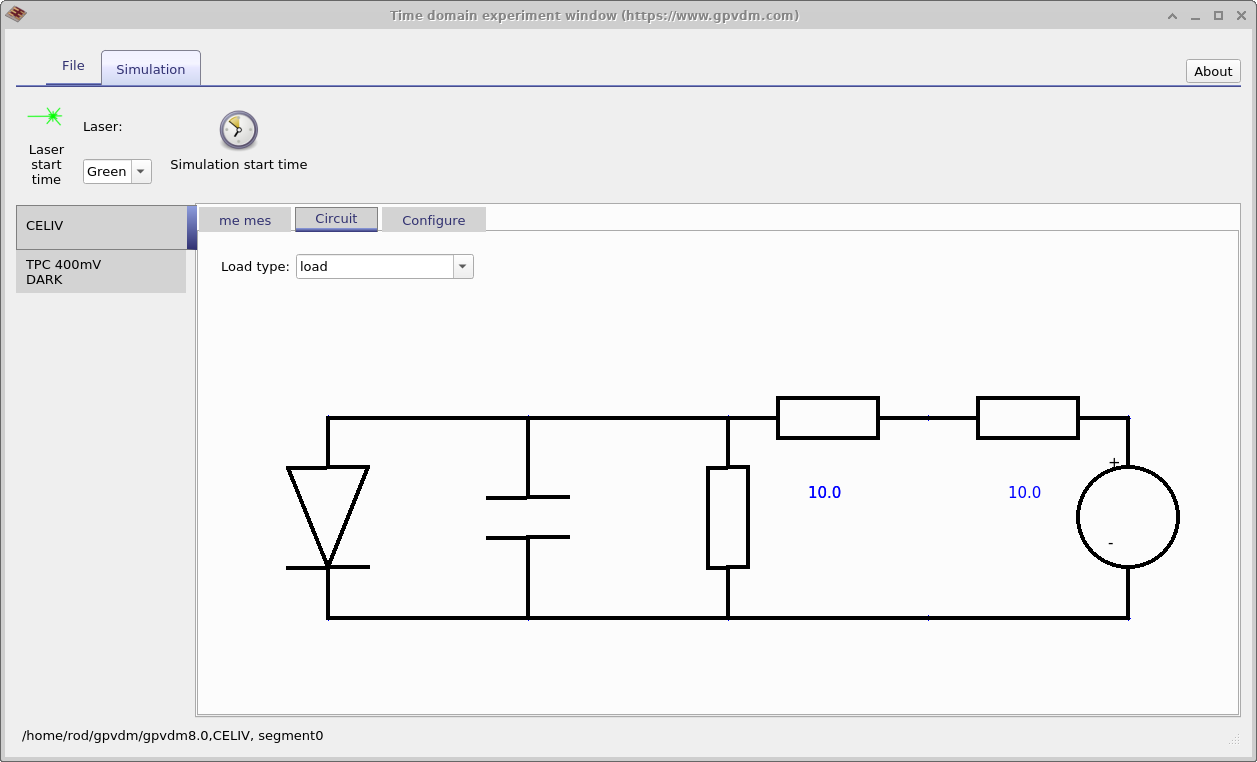
\includegraphics[width=0.5\textwidth,height=0.4\textwidth]{./images/time_domain_editor1.png}

&
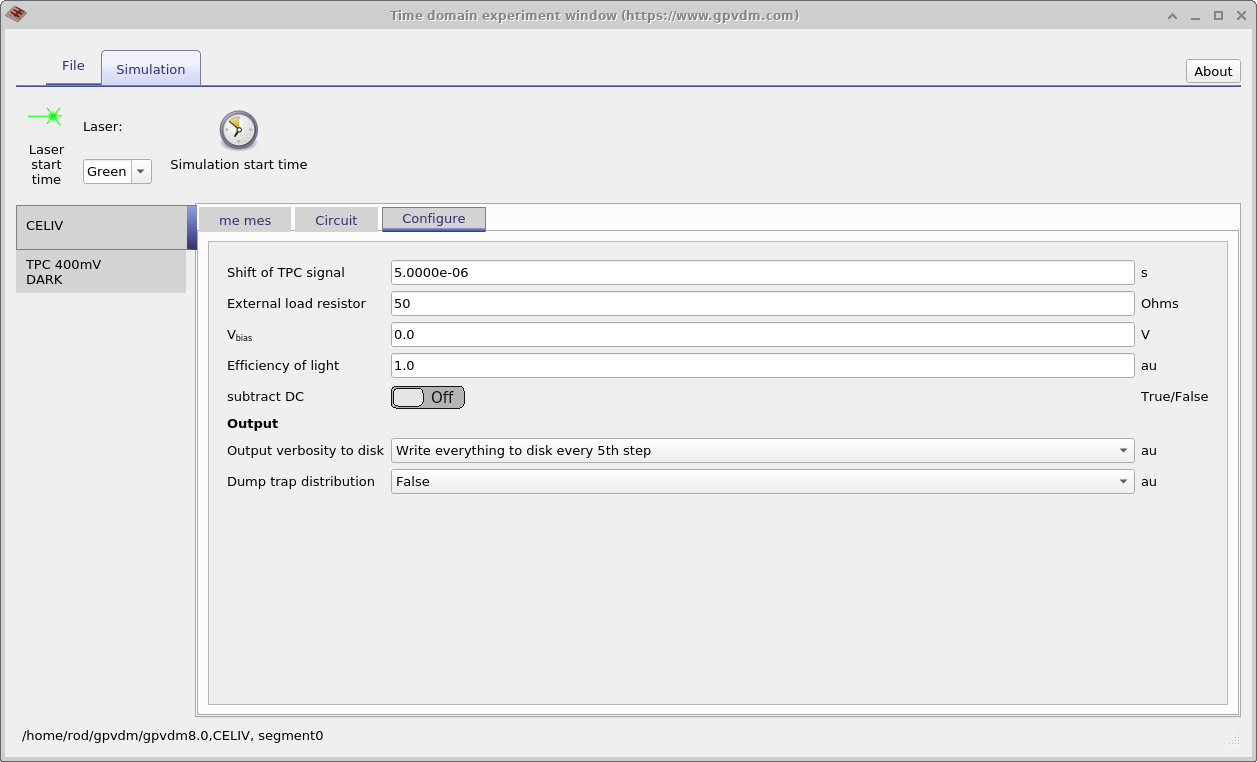
\includegraphics[width=0.5\textwidth,height=0.4\textwidth]{./images/time_domain_editor4.png}

\\

\end{tabular}
\caption{Configuring the time domain editor}
\label{fig:timedomaineditor2}
\end{figure}

\newpage
\section{Frequency domain editor}
Related YouTube videos:
\begin{figure}[H]

\begin{tabular}{ c l }


\includegraphics[width=0.05\textwidth]{./images/youtube.png}

&
\href{https://www.youtube.com/watch?v=NJAsZeiB5FU}{Simulating impedance spectroscopy (IS) in solar cells.}

\end{tabular}
\end{figure}

\subsection{Overview}
The frequency plugin allows you to simulate the frequency domain response of the device.  Using this tool one can perform impedance spectroscopy, as well as optically excited measurements such as Intensity Modulated Photo Spectroscopy (IMPS), Intensity Modulated Voltage Spectroscopy (IMVS). The  domain editor allows you to configure frequency domain simulations. This is shown below in Figures \ref{fig:fx_domain_mesh} and \ref{fig:fx_domain_circuit}. On the left hand side is the frequency domain mesh editor this is used to define which frequencies will be simulated.  Figure \ref{fig:fx_domain_circuit} shows the \emph{circuit} tab of the frequency domain window, this sets the electrical configuration of the simulation. One can either simulate an ideal diode (this is the fastest type of simulation to perform), a diode with parasitic components or a diode in open circuit. An ideal diode would be used for IMPS simulations while the open circuit model would be used for IMVS simulations. Pick the circuit depending on what conditions you want to simulate. If you want examples of frequency domain simulation look in the new simulation window under Organic Solar cells, some of the PM6:Y6 devices have examples of frequency domain simulations already set up.
\\
\\
\noindent
\begin{minipage}{0.5\textwidth}
	\centering
	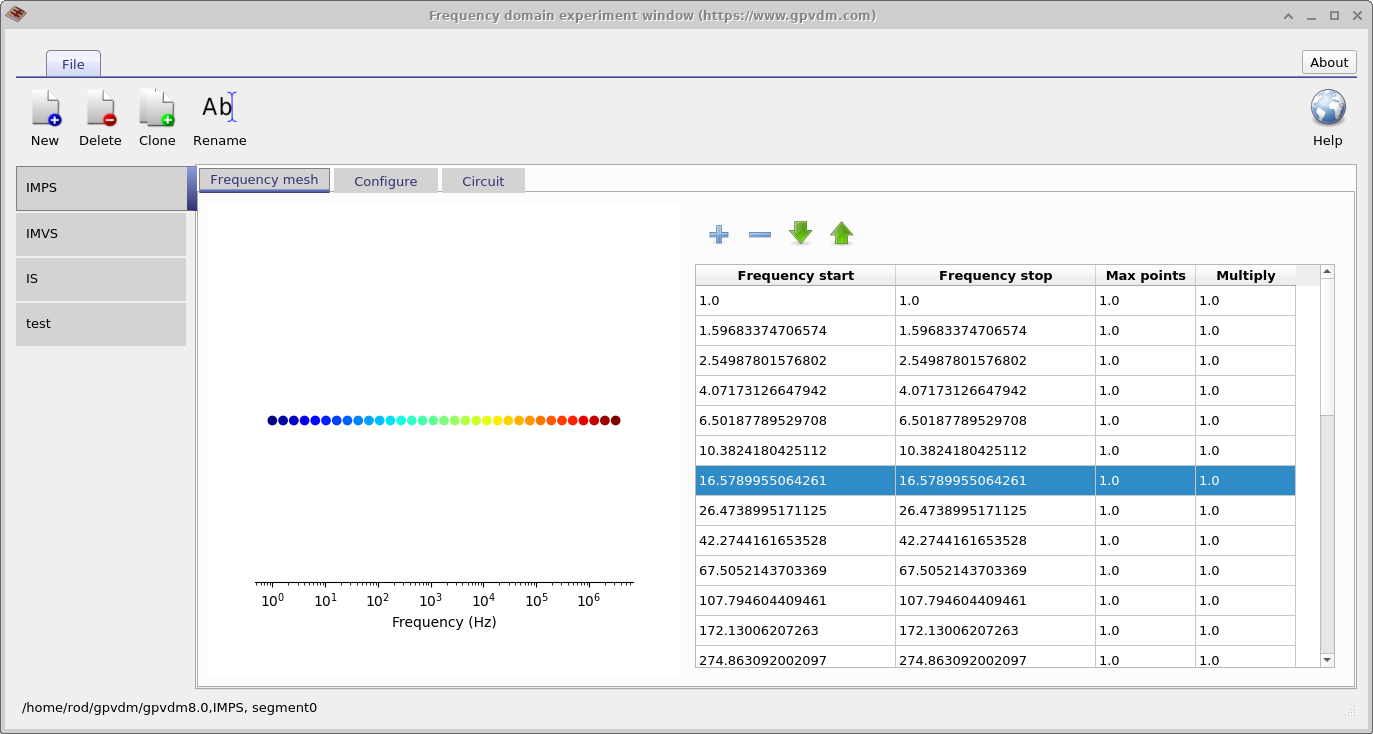
\includegraphics[width=\linewidth,height=0.8\linewidth]{./images/sim_editors/fx_domain_editor.png}
	\captionof{figure}{The frequency domain editor window}
	\label{fig:fx_domain_mesh}
\end{minipage}
\hspace{4pt}
\begin{minipage}[]{0.5\linewidth}
	\centering
	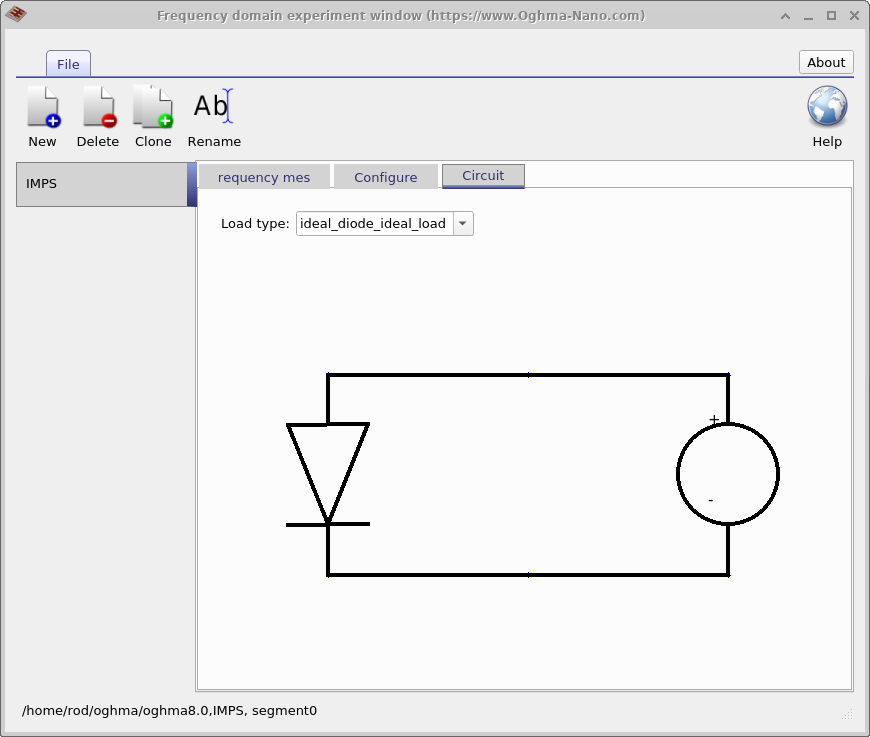
\includegraphics[width=\linewidth,height=0.8\linewidth]{./images/sim_editors/fx_domain_circuit.png}
	\captionof{figure}{A circuit set up for frequency domain simulations.}
	\label{fig:fx_domain_circuit}
\end{minipage}

\subsubsection{Large signal or small signal}
There are two ways to simulate frequency domain simulations in a device model, a large signal approach or a small signal approach. The small signal approach assumes the problem we are looking at varies linearly around a DC point, this may or may not be true depending on the conditions one is looking at. This method is however computationally fast.  The second approach is to use a large signal approach and rather than simulating linear variation around a set point one simulates the time domain response of the device in full for each wavelength of interest.  This method is cope better non-linear systems and one does not need to worry if one is in the large or small signal regime but is slower.  OghmaNano uses the large signal approach.

\subsection{Inputs}
In Figure \ref{fig:fx_domain_option} the \emph{Configure} tab of the frequency domain window can be seen. This decides exactly how the simulation will perform. These are described below in table \ref{tab:fx_inputs}

\begin{table}
\begin{center}
\begin{tabular}{ |l|p{8cm}| } 
 \hline
	File name 					& 	Description  \\ 
 \hline
	$V_{external}$				&	The external voltage applied to the cell\\ 
	Simulation type				&	Leave this as Large signal.\\
	Load resistor				&	External load resistor, this should be usually set to zero.\\ 
	FX domain mesh points 		&	The number of time steps used to simulate each cycle\\ 
	Cycles to simulate 			&	The number of complete periods of any given frequency that are simulated \\ 
	Excite with					&	How the device is excited, either optically or electrically.\\ 
	Measure 					&	What is measured, current or voltage.\\
	Modulation depth			&	How deep is the DC voltage/current modulated\\
 	Periods to fit				&	The number of frequency domain cycles that are fit to extract phase angle\\
 	Output verbosity to disk	&	How much data is dumped to disk (described in other sections)\\
 	Output verbosity to screen	&	How much data is shown on the creen (described in other sections)\\
 \hline
\end{tabular}
\caption{Files produced by the time domain simulation}
\label{tab:fx_inputs}
\end{center}
\end{table}

\begin{figure}
\centering
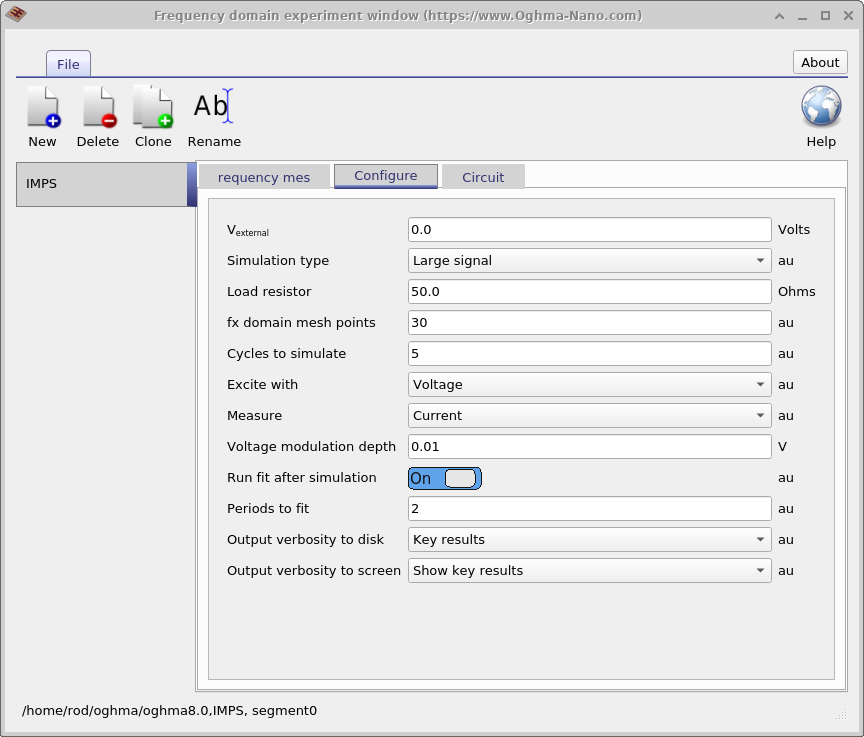
\includegraphics[width=0.7\linewidth,height=0.5\linewidth]{./images/sim_editors/fx_domain_options.png}
\caption{Configuring a frequency domain simulation}
\label{fig:fx_domain_option}
\end{figure}


\subsection{Outputs}


\begin{table}[H]
\begin{center}
\begin{tabular}{ |c|c|c| } 
 \hline
	File name 			& 	Description  \\ 
 \hline
	real\_imag.csv		&	Re(i(fx)) v.s. Im(i(fx))\\ 
	fx\_imag.csv		&	fx v.s. Im(i(fx))\\
	fx\_real.csv 		&	fx v.s. Re(i(fx))\\ 
	fx\_abs.csv 		&	fx v.s. $\lvert i(fx) \rvert$\\ 
	fx\_phi.csv 		&	fx v.s. $ \angle i(fx)$ \\ 
	fx\_C.csv 			&	fx v.s. Capacitance\\ 
	fx\_R.csv 			&	fx v.s. Resistance\\ 
 \hline
\end{tabular}
\caption{Files produced by the time domain simulation}
\label{tab:ce_output}
\end{center}
\end{table}


\clearpage
\section{Suns-Voc editor}
The Suns-Voc plugin can be used to calculate how open circuit voltage changes as a function of light intensity.  This can be useful for understanding tail slope and disorder in devices.  A picture of the suns-voc editor window can be seen below in figure \ref{fig:sunsvoceditor}.  The window can be used to set the start and stop light intensity. The Suns-Voc applies the voltage to the contact that is labelled \emph{Change}.

\begin{figure}[H]
\centering
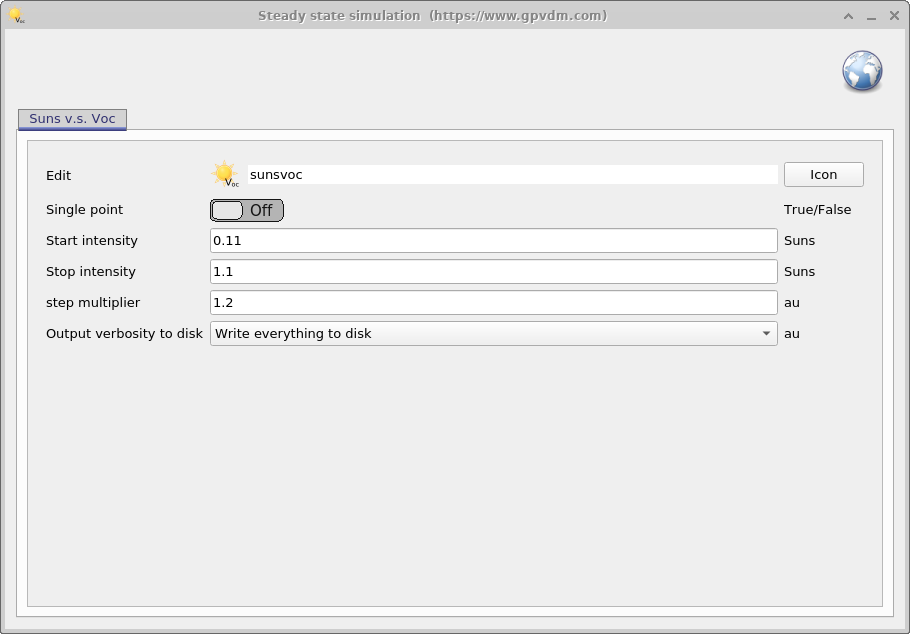
\includegraphics[width=0.7\textwidth,height=0.5\textwidth]{./images/sim_editors/suns_voc_editor.png}
\caption{The suns-voc editor window}
\label{fig:sunsvoceditor}
\end{figure}


\subsection{Outputs}

\begin{table}[H]
\begin{center}
\begin{tabular}{ |c|c| } 
 \hline
	File name 			& 	Description  \\ 
 \hline
	suns\_voc.csv 		&	Suns v.s. Voc curve \\ 
	suns\_Q.csv 		&	Suns v.s. Charge density\\ 
	suns\_mu.csv 		&	Suns v.s. average charge carrier mobility\\
	suns\_tau.csv 		&	Suns v.s. recombination constant tau \\ 
	Q\_Qtau.csv 		&	Charge density v.s. recombination constant tau \\
	Q\_mu.csv 			&	Charge density v.s. charge carrier mobility\\
	Q\_kbi.csv 			&	Charge density v.s. recombination prefactor kbi\\
	Q\_trap\_filling.csv &	Charge density v.s. fraction of filled traps\\
	V\_mu.csv 			&	Voc v.s. average charge carrier mobility\\
 \hline
\end{tabular}
\caption{Files produced by the Suns-Voc simulation}
\label{tab:suns_voc_output}
\end{center}
\end{table}


\newpage
\section{Suns-Jsc editor}
The Jsc editor can be used to configure suns-Jsc simulations. It enables you to set the start light intensity, stop light intensity and how big the steps are. This is shown in figure \ref{fig:sunsjsceditor}.

\begin{figure}[H]
\centering
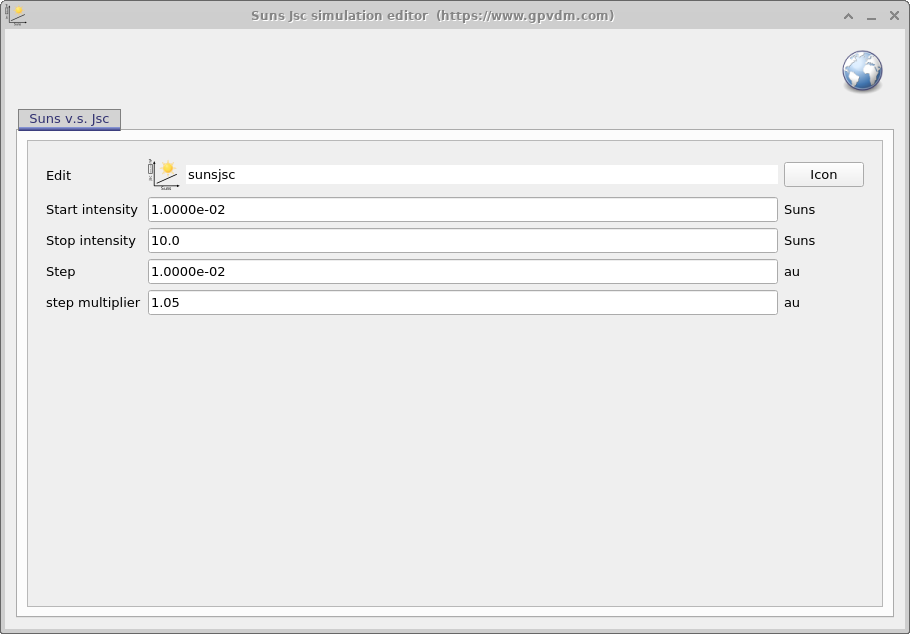
\includegraphics[width=0.7\textwidth,height=0.5\textwidth]{./images/sim_editors/suns_jsc_editor.png}
\caption{The JV curve editor window}
\label{fig:sunsjsceditor}
\end{figure}


\subsection{Outputs}

\begin{table}[H]
\begin{center}
\begin{tabular}{ |c|c| } 
 \hline
	File name 		& 	Description  \\ 
 \hline
	suns\_jsc.csv 	&	Suns v.s. Jsc curve \\ 
	suns\_mu.csv		&	Suns v.s. average charge carrier mobility \\ 
 \hline
\end{tabular}
\caption{Files produced by the Suns-Jsc simulation}
\label{tab:suns_jsc_output}
\end{center}
\end{table}

\clearpage
\section{Quantum efficiency editor}
The quantum efficiency editor simulates both EQE and IQE.  The configuration window can be used to set the voltage at which EQE and IQE are performed.
\begin{figure}[H]
\centering
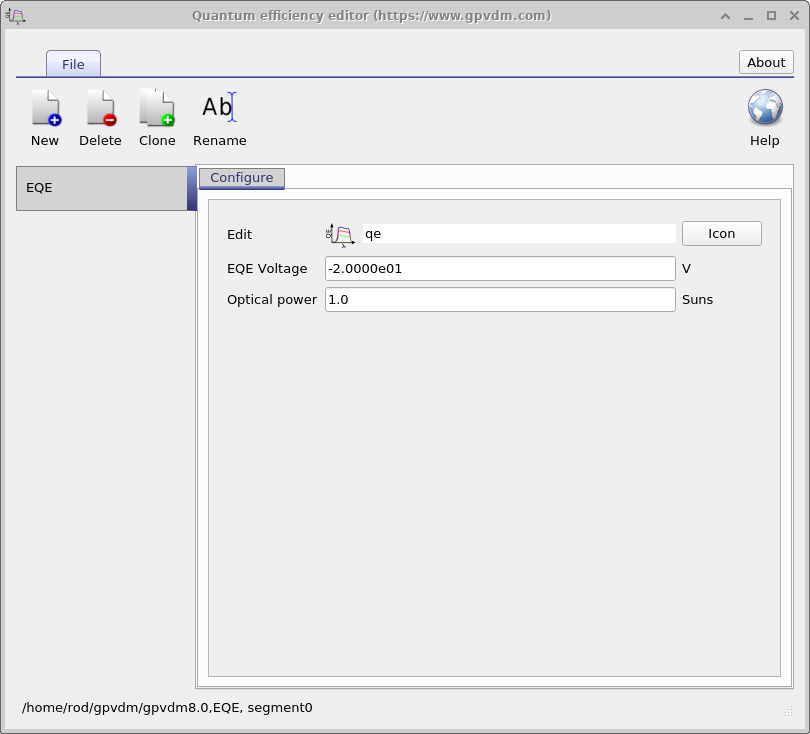
\includegraphics[width=0.7\textwidth,height=0.5\textwidth]{./images/sim_editors/qe_editor.png}
\caption{The quantum efficiency editor window}
\label{fig:qeeditor}
\end{figure}

\subsection{Outputs}

\begin{table}[H]
\begin{center}
\begin{tabular}{ |c|c| } 
 \hline
	File name 		& 	Description  \\ 
 \hline
	eqe.csv 		&	Wavelength v.s. EQE \\ 
	E\_eqe.csv		&	Photon energy v.s. EQE \\ 
	E\_eqe\_norm.csv	&	Photon energy v.s. Normalized EQE  \\ 
	iqe.csv			&	Wavelength v.s. IQE \\ 
	E\_iqe.csv		&	Photon energy v.s. IQE \\ 
	lam\_Gn.csv		&	Wavelength v.s. Average charge carrier generation rate \\ 
 \hline
\end{tabular}
\caption{Files produced by the Suns-Jsc simulation}
\label{tab:suns_jsc_output}
\end{center}
\end{table}

\newpage
\section{Scanning probe microscopy editor}
When simulating a 3D structure such as a large area contact one often wants to map the resistance between an x,z point on the surface of the device and the charge extraction contact. This tool is used to apply voltages systematically over z,x regions to map out voltage or resistance profiles in space.  This tool is usually used with either full 2/3D drift diffusion simulations or the 3D large area electrical circuit model. There is more about this tool in Section \ref{ref:la}.

\begin{figure}[H]
\centering
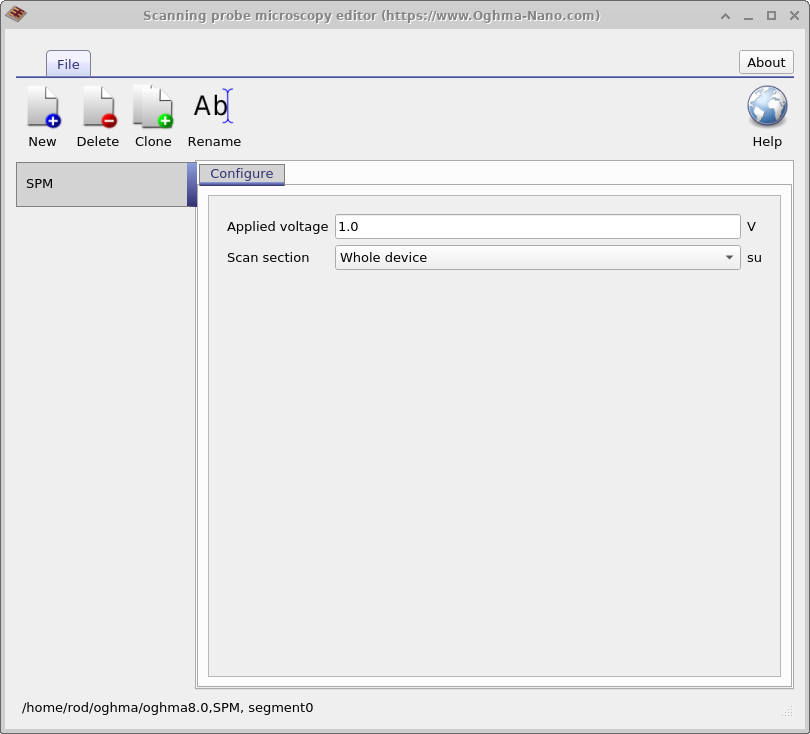
\includegraphics[width=0.7\textwidth,height=0.5\textwidth]{./images/sim_editors/spm.png}
\caption{The scanning probe microscopy editor}
\label{fig:spm_editor}
\end{figure}

\newpage
\section{Electrical equilibrium editor}
Sometimes when studding a device, it is not necessary to simulate an entire JV curve. One may for example just for example be interested in the band structure at 0V in the dark. The \emph{Electrical equilibrium} allows the user to setup simulations that only simulate the device at equilibrium (0V applied bias in the dark).

\begin{figure}[H]
\centering
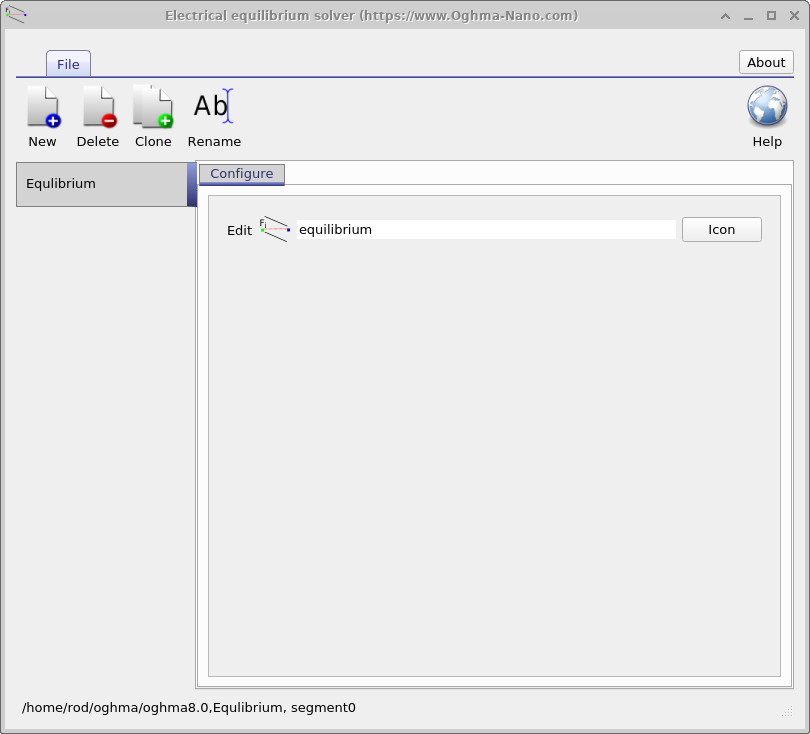
\includegraphics[width=0.7\textwidth,height=0.5\textwidth]{./images/sim_editors/equilibrium.png}
\caption{Electrical equilibrium editor}
\label{fig:equilibrium_editor}
\end{figure}

\newpage
\section{Steady state photoluminencense editor}
This tool is used to generate photoluminencense spectra at a desired voltage, either short circuit or open circuit.

\begin{figure}[H]
\centering
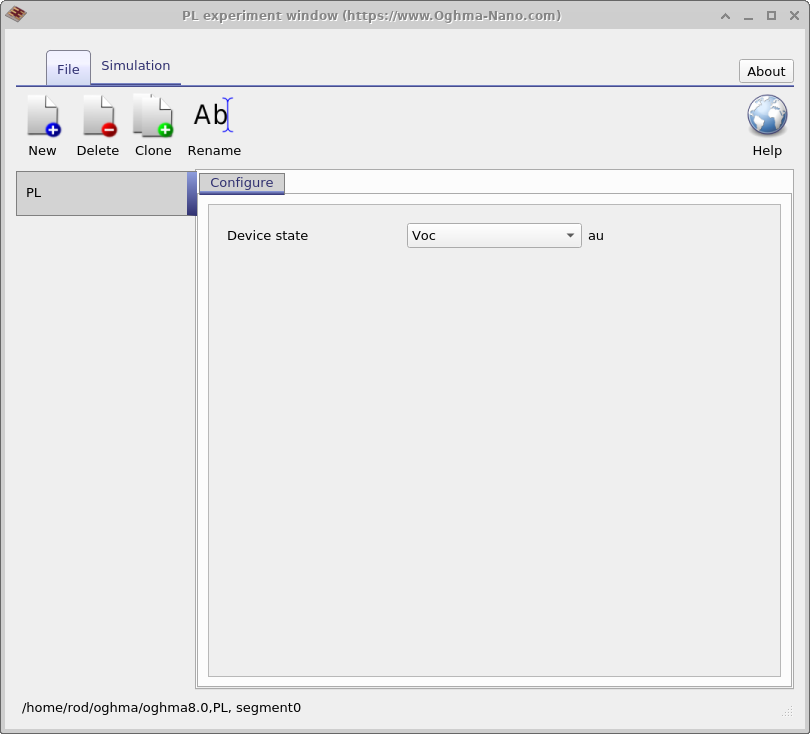
\includegraphics[width=0.7\textwidth,height=0.5\textwidth]{./images/sim_editors/pl.png}
\caption{Steady state photoluminencense editor}
\label{fig:pleditor}
\end{figure}

\newpage
\section{Charge extraction editor}
\noindent
\begin{minipage}{0.5\textwidth}
This is the charge extraction editor, it allows one to simulate charge extraction transients. A charge extraction experiment is performed to find out how much charge is in a disordered device. For this type of experiment one runs the device at a set voltage and light intensity say 1V @ 1Sun. Then one turns off the light and shorts the cell through a resistor and integrates the total current outputted by the cell to get the charge that was in the cell when it was operating. Typically the cell is shorted through the the 50 Ohm termination of an oscilloscope so that by measuring the voltage transient and applying V=IR one can calculate the current and thus total charge.
\end{minipage}
\hspace{4pt}
\begin{minipage}[]{0.5\linewidth}
	\centering
	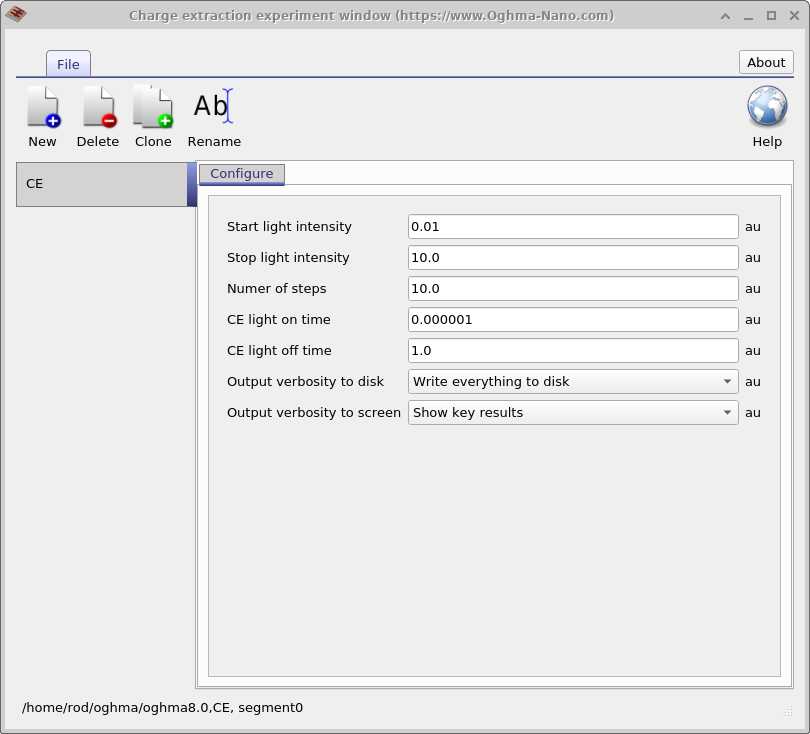
\includegraphics[width=\linewidth,height=0.8\linewidth]{./images/sim_editors/ce.png}
	\captionof{figure}{Charge extraction editor}
	\label{fig:ce_editor}
\end{minipage}
\\
\\
 This type of measurement is important in disordered devices when one wants to find out how much charge is in the trap states.  It is important to note that the experiment does not extract all the charge in the device, it only extracts the difference between charge at operating conditions and 0V @ 0 Suns. The background charge due to injection from the contacts/doping is still left in the device. There is also error loss in the CE experiment due to recombination annihilating charge before it has left the device.


\subsection{Outputs}


\begin{table}[H]
\begin{center}
\begin{tabular}{ |c|c|c| } 
 \hline
	File name 			& 	Description  \\ 
 \hline
	$time\_i.csv$ 		&	Time v.s. extraction current for a single CE experiment\\ 
	$time\_v.csv$ 		&	Time v.s. voltage for a single CE experiment\\ 
	$suns\_Q\_ce.dat$ 	&	Suns v.s. extracted charge including effects of recombination\\ 
	$v\_np.dat$ 			&	Voltage c.s. extracted charge including the effects of recombination \\
	$suns\_np.dat$ 		&	Suns c.s. extracted charge including the effects of recombination   \\
	$v\_np\_ideal.dat$ 	&	Voltage v.s. extracted charge not including the effects of recombination\\
	$suns\_np\_ideal.dat$ &	Suns v.s. extracted charge not including the effects of recombination\\
 \hline
\end{tabular}
\caption{Files produced by the charge extraction simulation}
\label{tab:ce_output}
\end{center}
\end{table}

\clearpage
\section{Capacitance voltage editor}
Experimentally capacitance voltage (CV) measurements are a useful way to determine doping within a device. In OghmaNano CV measurements use a cut down version of frequency domain simulation tool described above.

\begin{figure}[H]
\centering
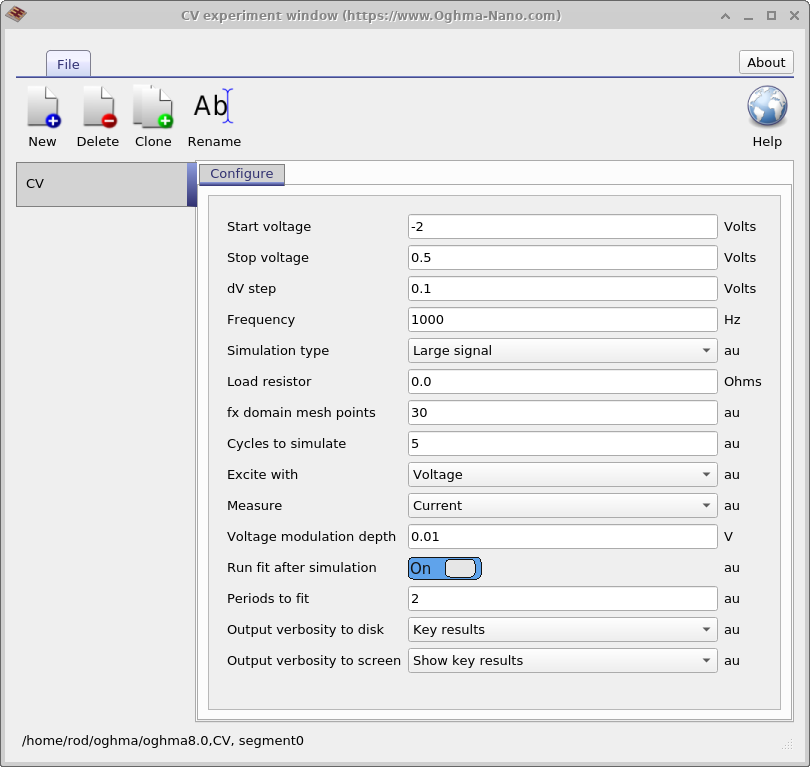
\includegraphics[width=0.7\textwidth,height=0.5\textwidth]{./images/sim_editors/cv.png}
\caption{The capacitance voltage editor}
\label{fig:cv_editor}
\end{figure}

\subsection{Outputs}

\begin{table}[H]
\begin{center}
\begin{tabular}{ |c|c| } 
 \hline
	File name 		& 	Description  \\ 
 \hline
	real\_imag.dat 		&	Re(i(fx)) v.s. Im(i(fx)) \\ 
	fx\_real.dat 		&	fx v.s. Re(i(fx)) \\ 
	fx\_imag.dat 		&	fx v.s. Im(i(fx)) \\ 
	cv.dat 				&	fx v.s. Capacitance \\ 
	cv2.dat 			&	fx v.s. $1/{Capacitance}^2$ \\ 
 \hline
\end{tabular}
\caption{Files produced by the CV simulation}
\label{tab:suns_jsc_output}
\end{center}
\end{table}

\clearpage
\section{Hardware editor}
All computer programs including OghmaNano run on physical computing hardware. There are may combinations of hardware that can be in any computer, some computes have a large number of CPU cores while others only have one. Likewise computers come with differing amounts of memory, hard disk space and GPUs. To help the user get the best out of OghmaNano, there is a hardware editor where the user can configure how OghmaNano behaves on any given computer. This can be accessed through the simulation tab window see Figure \ref{fig:hardware_ribbon}. 

\begin{figure}[H]
\centering
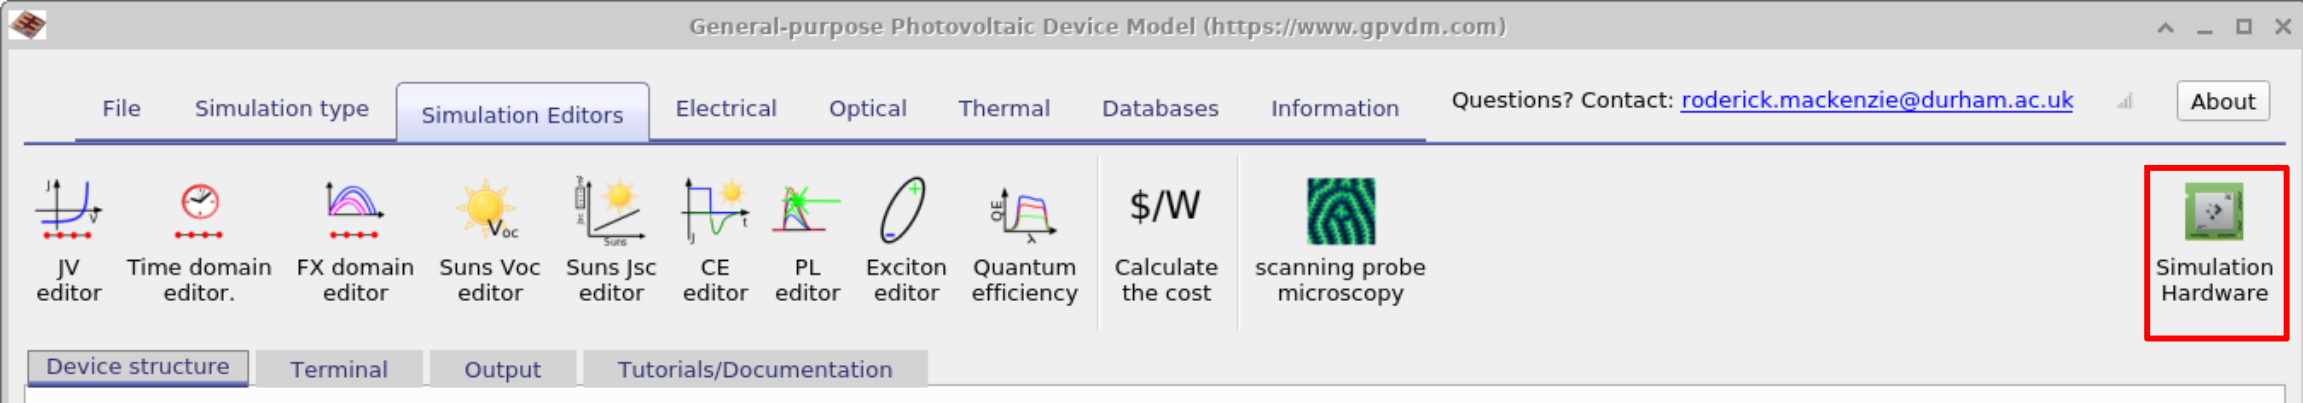
\includegraphics[width=0.9\textwidth,height=0.15\textwidth]{./images/sim_editors/ribbon_hardware.png}
\caption{Opening the hardware editor.}
\label{fig:hardware_ribbon}
\end{figure}

If you click on this it will bring up the hardware editor window which can be seen in Figure \ref{fig:hardware_editor}

\begin{figure}[H]
\centering
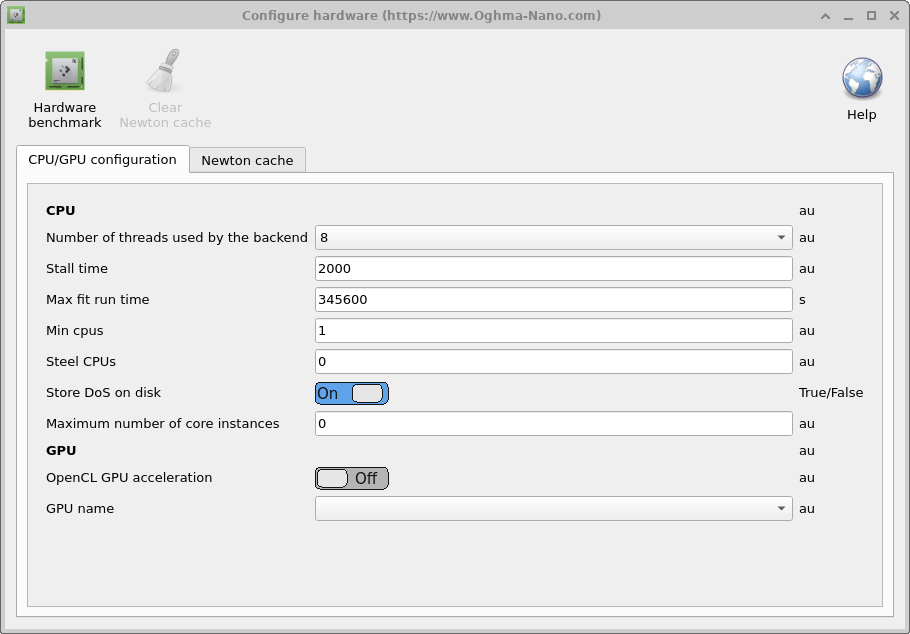
\includegraphics[width=0.7\textwidth,height=0.5\textwidth]{./images/hardware/cpu.png}
\caption{The hardware editor window}
\label{fig:hardware_editor}
\end{figure}

The hardware window is comprised of various tabs which enable the user to edit the configuration and also benchmark your device. 

\subsection{CPU/GPU configuration tab}
This tab is used to configure how OghmaNano interacts with the GPU and CPU it is described in the table below. As described in other parts of this manual in detail there are two parts to OghmaNano there is oghma\_core.exe which is the computational back end and there is oghma\_gui.exe which is the graphical user interface, how both these parts of the model behave can be fine tuned here.

	\begin{itemize}
		\vspace{-0.2cm}\item \emph{Number of threads used by the backend:} This is the maximum number of threads OghmaNano oghma\_core.exe can use. This dictates; the number of simultaneous fits that can be run; the maximum number of optimization simulations that can be run at the same time; the maximum number of threads that are used for FDTD simulations; maximum number of of DoS cache files can generated at the same time; number of frequency domain points that can be run at the same time.
		\vspace{-0.2cm}\item \emph{Maximum number of core instances:} This sets the maximum number of oghma\_core.exe instances that can be started by the GUI. If one is running a parameter scan then this will control the maximum number of simultaneous simulations that can be performed at the same time. If the values of \emph{Number of threads used by the backend} has been set to 4 and one is performing an FDTD simulation, then one sets \emph{Maximum number of core instances} to 8, then the GUI will spawn 8 instances of oghma\_core.exe each using 4 threads, thus 32 CPU cores will be needed.
		\vspace{-0.2cm}\item \emph{Stall time:} Sometimes when running OghmaNano on a supercomputer unattended it can stop running, possibly because of an IO error or network error. This option can be used to set the maximum length of a single simulation. By single simulation I mean a single JV curve, single time domain simulation or single frequency domain simulation, but not a whole fit which will involve running thousands if individual simulations.). So with a value of 2000 seconds the solver will exit, if for example a single JV simulation takes longer than 2000 seconds. In reality any individual simulation should take only a few seconds, so this option acts as a hard backstop if something has gone very wrong. 
		\vspace{-0.2cm}\item \emph{Max fit run time:} This is the maximum time oghma\_core.exe can reside in memory. If any simulation or fit takes longer than this value it will be terminated, again this is a backstop to prevent simulations running forever.  The default value is 4 days. 
		\vspace{-0.2cm}\item \emph{Steel CPUs:} Sometimes when running OghmaNano on a shared PC one will set a simulation running when another user is using a significant number of cores. After a while the other user's simulations will finish running leaving the computer with idling CPUs. If this option is set to \emph{True}, then OghmaNano will monitor the number of free CPUs and if more become available it will use them.
		\vspace{-0.2cm}\item \emph{Min CPUs:} Used with the option above \emph{Steel CPUs} to set the minimum number of CPUs that will be used.
		\vspace{-0.2cm}\item \emph{Store DoS on disk:} OghmaNano stores lookup tables on disk to speed up simulations, if this option is set to false these lookup tables will not be stored.
		\vspace{-0.2cm}\item \emph{OpenCL GPU acceleration:} This enables or disables GPU acceleration, this is used mainly during the FDTD simulations.
		\vspace{-0.2cm}\item \emph{GPU name:} Selects the GPU to use.
	\end{itemize}

\subsection{Newton cache}

When running simulations with a significant number of ODEs, such as 1D devices with a lot of trap states and a lot of spatial points, or when running 2D OFET simulations each voltage step can take a while to compute. This is because the solver must solve each voltage step using Newton's method until it converges. For each each solver step the Jacobian must be built, the matrix inverted multiplied by the residuals and updates to all solver variables calculated. This can take a significant amount of time per step (2000ms). An approach to side step this approach is to store previously calculated answers on disk and then when the user asks the solver to calculated an already calculated problem the answer can be recalled rather than recalculated. This is very useful in OLED design where one is trying to optimise the optical structure of the device but leaves the electrical structure unchanged. One can run new optical simulations with already pre-calcualted electrical solutions.  Configuration options are displayed in the table below.

There is an overhead to using the Newton Cache, so I would only recommend it when solving the electrical problem is very slow indeed. Technically the Newton cache works by taking the MD5 sum of the Fermi-levels and the potentials to generate a hash of the electrical problem. This is then compared to what exists on disk. If a precalculated answer is found, the Fermi-levels/potentials are updated to the values found on disk. The cache is stored in oghma\_local\\cache, each pre solvedsolution is stored as a new binary file. Each simulation run generates an index file where all MD5 sums from that simulation are stored. Once the cache becomes full OghmaNano deletes simulation results in batches based on the index files.

\begin{figure}[H]
\centering
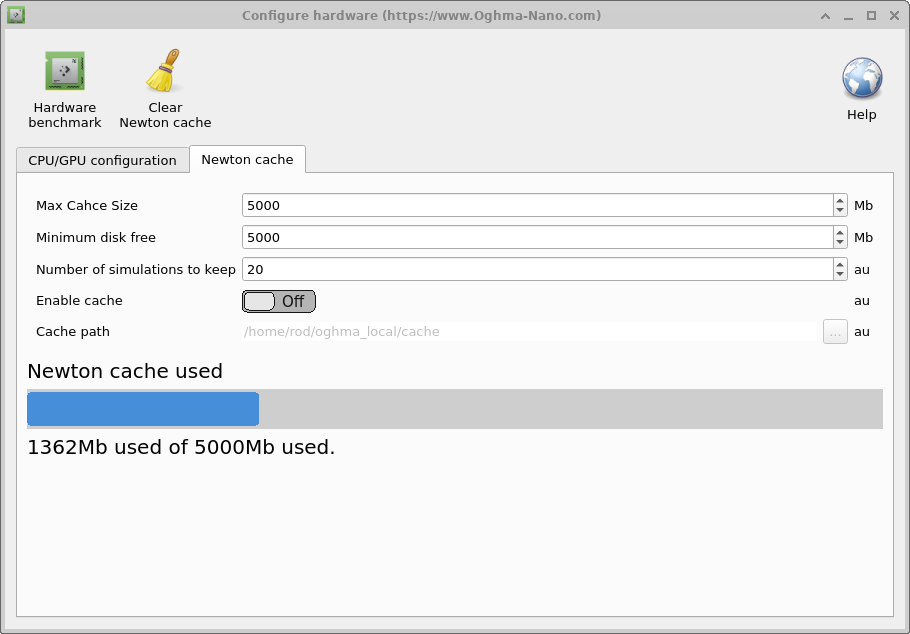
\includegraphics[width=0.7\textwidth,height=0.5\textwidth]{./images/hardware/newton.png}
\caption{The Newton cache editor}
\label{fig:newton_cache_editor}
\end{figure}


	\begin{itemize}
		\vspace{-0.2cm}\item \emph{Maximum cache size:} Sets the maximum size of the cache in Mb. I would recommend around 1Gb.
		\vspace{-0.2cm}\item \emph{Minimum disk free:} Sets the minimum amount of disk space needed to use the cache, this option is designe dto prevent the cache filling the disk I would set it to around 5Gb.
 		\vspace{-0.2cm}\item \emph{Number of simulations to keep:} This will set the maximum number of simulation runs to keep, I would set it to between 20 and 100.
 		\vspace{-0.2cm}\item \emph{Enable cache:} This enables or disables the Newton Cache, the default and recommended option is False.
	\end{itemize}

\subsection{Hardware benchmark}
In the top left of hardware window \ref{fig:newton_cache_editor} there is a button called \emph{Hardware benchmark}. If this is clicked then OghmaNano will benchmark your hardware, the result of such a benchmark can be seen in \ref{fig:hardware_benchmark}. This runs benchmarks your CPUs ability to calculate \emph{sin},\emph{exp} and allocate/deallocate memory in blocks. It displays how long it took to do a few thousand operations as well as an \emph{R} (aka Roderick) value. This is defined as R=\emph{Time taken to do the calculation on your PC}/\emph{The time take to do the calculation on my PC}. Thus smaller values mean your PC is faster than mine. My PC is a Intel(R) Core(TM) i7-4900MQ CPU @ 2.80GHz in a 2017 Lenovo thinkpad. So most modern computers should be faster. If you have good CPU performance but your simulations are running slower than my YouTube videos then this is invariably due to bad IO speed, caused by virus killers, storing the simulations on OneDrive, using networked drives, using slow USB storage etc.

\begin{figure}[H]
\centering
\includegraphics[width=1.0\textwidth,height=0.8\textwidth]{./images/hardware/benchmark.png}
\caption{Running a hardware benchmark}
\label{fig:hardware_benchmark}
\end{figure}




\chapter{2D simulations - OFETs}
\label{sec:ofet}

\begin{figure}[H]

\begin{tabular}{ c l }

\includegraphics[width=0.05\textwidth]{./images/youtube.png}

&
\href{https://www.youtube.com/watch?v=0RK9GEyb4HQ}{Tutorial on OFET simulation.}

\end{tabular}
\end{figure}

Gpvdm contains a 2D electrical solver which can be used for simulating OFETs and other 2D structures.  To perform 2D simulations use the default OFET simulation in gpvdm as a starting point.  You can do this by double clicking on \emph{OFET simulation} in the new simulation window (see figure \ref{fig:ofetnewsim}).
\\
\\
\fbox{
\parbox{0.9\textwidth}{
\color{black} Note: The 2D electrical solver is a separate plug in to the 1D solver, if you select the default OFET simulation gpvdm as a starting point for your own 2D simulations gpvdm will be all set up to do 2D electrical simulations.  If you try to convert a 1D simulation such as a solar cell to a 2D simulation (not recommended) please read section \ref{sec:solverconfig} on how to select the correct solver.
}\par
}
\\
\\




To make a new OFET simulation, click on the new simulation button. In the new simulation window and select the OFET simulation (see figure \ref{fig:ofetnewsim}).  This will bring up the initial OFET simulation shown in figure \ref{fig:ofetstartsim}.

\begin{figure}[H]
\centering
\includegraphics[width=0.7\textwidth]{./images/ofet_0.png}
\caption{Opening a new ofet simulation}
\label{fig:ofetnewsim}
\end{figure}




\subsection{The anatomy of a 2D simulation}

\begin{figure}[H]
\centering
\includegraphics[width=0.7\textwidth]{./images/ofet_1.png}
\caption{The default ofet simulation.}
\label{fig:ofetstartsim}
\end{figure}

The OFET structure shown in figure \ref{fig:ofetstartsim} consists of a \emph{gate} and \emph{drain} contact shown on the top of the simulation as gold bars, a semiconductor layer is shown in blue and an insulating later shown in red.  A \emph{gate} contact is also visible at the bottom of the structure.  This layer structure is defined in layer editor, see figure \ref{fig:ofetlayerstructure}. The layer editor has been described in detail in section \ref{sec:layereditor}. It can be seen that the top and bottom layers have been set to \emph{contact} and the insulator (PMMA) and semiconducting layer have been set to active. This means that the drift diffusion equations will be solved over the semiconductor and insulator layers and the contacts will be used as boundary conditions.  As this structure is not emitting light the \emph{Optical material} column has no impact on the simulation results.

%\fbox{
%\parbox{0.9\textwidth}{
%\color{blue} Task \addtocounter{question}{1}\thequestion : Try changing the heigh of the gate layer from 100nm to 500 nm and see what ahpp
%}\par
%}
%\\


\begin{figure}[H]
\centering
\includegraphics[width=0.7\textwidth]{./images/ofet_2.png}
\caption{The layers of an OFET device}
\label{fig:ofetlayerstructure}
\end{figure}

The contacts are defined in the contact editor shown in figure \ref{fig:ofetcontacteditor}. The contact editor has been described in detail in 
section \ref{sec:contacteditor}, however because this is a 2D simulation another two extra columns have appeared. They are \emph{start} and \emph{width}.  These define the start position of the contact on the x-axis and width which describes the width of the contact on the x-axis.  The \emph{source} starts at $0~m$ and extends to $5 \mu m$, the  \emph{drain} starts at $75~\mu m$ and extends to $5 \mu m$, while the gate starts at $0~m$ and extends to cover the entire width of the device which is $80~ \mu m$.  If you are unsure which is the x-axis, the origin marker is visible at the bottom of figure \ref{fig:ofetstartsim}.

\begin{figure}[H]
\centering
\includegraphics[width=0.7\textwidth]{./images/ofet_3.png}
\caption{Editing the contacts on a 2D device.}
\label{fig:ofetcontacteditor}
\end{figure}

The electrical parameters for both the semiconductor and the insulator can be seen in figure \ref{fig:ofetelectricalparamters}, these can be accessed through the \emph{Electrical parameter} editor. The \emph{Electrical parameter} editor is described in detail in section \ref{sec:doseditor}. To the left of the figure the parameters for the semiconducting layer are described and to the right of the figure the parameters for the insulating layer are described. Below I have made comments on each parameter in relation to OFET simulation.

\begin{itemize}
  \item Mobility: The free carrier mobility in the active layer will be defined by the semiconductor you are trying to simulate.  The mobility in the insulator is usually set to a low value such as $1e-12-1e-15$ to limit current flow into the region. However, the value should not be set too low (see section \ref{sec:solverstability}) or the solver may become numerically unstable.
  \item Effective density of states: Keep these the same for both layers, just to keep things simple.
  \item Number of trap states: You can set this to what value you want to but if you choose a large number in 2D it will significantly affect the speed of the simulation, simply because \emph{number of equation solved=XMESHPOINTS $\times$ YMESHPOINTS $\times$ NUMEROFTRAPS}.
  \item Eg and Xi: Although it is tempting to simply enter the experimental values for Xi and Eg for both the insulator and the semiconductor, one has to be careful in doing this as some insulators ($SiO_2$) have very big band gaps which mean the number of carriers get very small and make the simulation unstable (read section \ref{sec:solverstability} for an explanation).  If you want to simulate a jump in the band gap into an insulator, my is to make the jump significantly bigger than $3/2kT=25meV$ which is the average kinetic energy of a charge carrier.  If the gap is between $0.5-1.0 V$ charge carriers will have problems penetrating the barrier and there is no need to simulate bigger steps.
\end{itemize}

\begin{figure}[H]
\centering
\begin{tabular}{ c c }

\includegraphics[width=0.5\textwidth,height=0.4\textwidth]{./images/ofet_5.png}

&
\includegraphics[width=0.5\textwidth,height=0.4\textwidth]{./images/ofet_6.png}
\\
\end{tabular}
\caption{Electrical parameters for both the semiconductor (left) and the insulator (right)}
\label{fig:ofetelectricalparamters}
\end{figure}

\subsection{Running a 2D simulation}

2D simulations are run in the same way as 1D simulations, simply click on the play button, see figure \ref{fig:ofetrun}.
\begin{figure}[H]
\centering
\includegraphics[width=0.7\textwidth]{./images/run_sim.png}
\caption{Running an OFET simulation}
\label{fig:ofetrun}
\end{figure}

The simulation will take longer than it's 1D counterparts simply because there will be more equations to solve.  If you have set a contact at a high starting voltage the solver will initially ramp the contact voltage in a stepwise way until the desired voltage is achieved before the desired voltage sweep is applied to the \emph{active contact}. After the simulation has run the following files will be produced showing the current density from each contact.


\begin{itemize}
  \item contact\textunderscore iv0.dat:
  \item contact\textunderscore iv1.dat:
  \item contact\textunderscore iv2.dat:

  \item contact\textunderscore jv0.dat:
  \item contact\textunderscore jv1.dat:
  \item contact\textunderscore jv2.dat:

  \item snapshots:

\end{itemize}

\begin{figure}[H]
\centering
\begin{tabular}{ c c }

\includegraphics[width=0.5\textwidth,height=0.4\textwidth]{./images/ofet_7.png}

&
\includegraphics[width=0.5\textwidth,height=0.4\textwidth]{./images/ofet_8.png}
\\

\includegraphics[width=0.5\textwidth,height=0.4\textwidth]{./images/ofet_9.png}

&
\includegraphics[width=0.5\textwidth,height=0.4\textwidth]{./images/ofet_10.png}
\\
\end{tabular}
\caption{Electrical parameters}
\end{figure}

\subsection{Meshing in 2D}

\begin{figure}[H]
\centering
\includegraphics[width=0.7\textwidth]{./images/ofet_4.png}
\caption{Meshing}
\label{fig:ofetmeshing}
\end{figure}










\chapter{2D simulation of bulk-heterojunctions}
\label{sec:bhj}

\begin{figure}[H]
\begin{tabular}{ c l }

\includegraphics[width=0.05\textwidth]{./images/youtube.png}

&
\href{https://www.youtube.com/watch?v=dlEscq1WSJQ}{Simulating 2D BHJ structures in OghmaNano}

\end{tabular}
\end{figure}

To be written but there is an example simulation in the new simulation window.


\chapter{Meshing}
\label{ref:mesh}

\section{What is meshing?}
Meshing is the process of taking a continuous problem space, say a bar along which heat is conducted form a candle to a block of ice and turning this into a discrete computational problem.  This usually involves picking a series of points along this space and using these to represent the entire problem (see Figure \ref{fig:emeshdiagram}). The reason we need to break a region up into points to model it is because computers have finite memory and can not model a continuum very easily. If you want more details why and how this is done search for basic finite difference tutorials on the web.

\begin{figure}[H]
\centering
\includegraphics[width=\textwidth]{./images/mesh/general_mesh_diagram.png}
\caption{An example of a continuous problem broken up (or meshed) into a series of discrete points.}
\label{fig:emeshdiagram}
\end{figure}

\section{Different meshes for different problems}

In simple terms OghmaNano solves three physical models, the optical model describing light, the thermal model describing thermal effects and the electrical model describing electrical effects. The physical effects from each of these three models often happen on different length scales so need different meshes. For example:

\begin{itemize}
  \item Electrically interesting effects may only happen in the active layer of a solar cell (100 nm thick), so it is only worth solving the drift diffusion equations in this layer, however light interacts with all layers in the cell (1 $\mu$m thick) so the optical problem should be solved over the entire device. This means light should be modelled covering the whole device but electrical effects only in the active layer.
  \item A Quantum Well laser diode used for cutting steel may generate a lot of heat in it's Quantum Well (30 nm thick) and waveguide layers (1 $\mu$m) thick but heat will escape from device through a heat sink which may be a 1 cm thick block of copper. This means electrical effects should be modelled within the device on (1 $\mu$m) scale the but thermal effects should be modelled on the cm scale.
\end{itemize}

Thus different effects need to be simulated on different length scales. Furthermore, you electrical device structure may have some very thin layers such as contact layers or interface layers which are only a few nanometres thick. Optically these layers are far below the wavelength of light so you don't need to worry about them from the optical perspective, but electrically they are very important as they define the current voltage characteristics of the device. Thus you would want to use a very fine electrical mesh over the layer to make sure they were modelled accurately from the electrical stand point but you could use a very wide optical mesh that skips the layers. 

In general OghamNano interpolates between the three meshes, so for example if you set up an thermal profile using a temperature mesh, and the temperature values are needed in the electrical problem the values are transferred through interpolation. You don't need to worry about this as a user. The same is true for the optical simulation values of Generation rate etc. are interpolated between from the optical mesh to the electrical mesh as needed.

\section{The three meshes of OghmaNano}
The thermal, optical and electrical ribbons are shown below in Figure \ref{tab:mesh_ribbons},  it can be seen that in each of these ribbons is a a mesh button, where the thermal, optical and electrical meshes can be defined.

\begin{figure}[H]
\centering
\begin{tabular}{ c }
\includegraphics[width=0.9\textwidth,height=0.1\textwidth]{./images/mesh/mesh_0.png}  \\
\includegraphics[width=0.9\textwidth,height=0.1\textwidth]{./images/mesh/mesh_1.png}  \\
\includegraphics[width=0.9\textwidth,height=0.1\textwidth]{./images/mesh/mesh_2.png}  \\
\end{tabular}
\caption{The thermal, electrical and optical ribbons.}
\label{tab:mesh_ribbons}
\end{figure}


\subsection{Electrical mesh}
If you click on the electrical mesh button in the electrical ribbon of the main window a window looking like Figure \ref{fig:emesh} will appear. The buttons marked 1D, 2D and 3D at the top of the window in Figure \ref{fig:emesh} can be used to toggle the simulation between 1D, 2D and 3D modes.  In this example the mesh is set up for a 2D OFET simulation, so \emph{y} and \emph{x} are depressed. Note, if you want to do 2D or 3D simulations you are best off using a default 2D simulation, such as the OFET simulation.  This is because to do 2D/3D simulations, a special newton solver configuration will be needed. The tables that looks like a spreadsheet is used to configure the mesh. The columns \emph{thickness} and \emph{mesh points}, determine the thickness of the mesh layer and the number of points on the mesh layer. The column, \emph{step multiply} by how much to grow each step.  For the second row of the x mesh the step multiplier is set to 1.1 which means the distance between the points will grow by 10\% each mesh point. The buttons marked left/right, defines on which side the mesh layer is generated from.  The resulting meshes are plotted in the graphs at the bottom of the window.

\begin{figure}[H]
\centering
\includegraphics[width=0.8\textwidth]{./images/mesh/electrical_mesh_window.png}
\caption{The electrical mesh editor showing the mesh for a 2D OFET simulation.}
\label{fig:emesh}
\end{figure}

The button called \emph{Import from layer editor} clears the y-electrical mesh and imports all the layers from the layer editor giving them four mesh points each. This is useful when setting up complex structures with many layers such as laser diodes.
 
\subsection{Optical mesh}
The optical mesh window is shown below in Figure \ref{fig:optical_mesh}, this is more or less identical to the electrical mesh window except it also has a panel to configure which wavelengths are simulated in a simulation. These wavelengths are used in ray tracing, FTDT simulations and transfer matrix simulations. In any simulation where a wavelength range is defined this mesh will be used.

\begin{figure}[H]
\centering
\includegraphics[width=0.8\textwidth]{./images/mesh/optical_mesh_window.png}
\caption{The optical mesh editor showing the number of points in position space and the number of wavelength points used for the optical simulations.}
\label{fig:optical_mesh}
\end{figure}

\subsection{Thermal mesh}
This will generally be handled automaticity for you. And you will only need to consider the thermal mesh when you turn on self heating in the device. Some parameters such as 
 
\section{The electrical mesh in detail}
A picture of the electrical mesh is given below \ref{fig:electrical_mesh_diagram} note the mesh does not start at zero but half a mesh point into the device.

\begin{figure}[H]
\centering
\includegraphics[width=0.8\textwidth]{./images/mesh/electrical_mesh_diagram.png}
\caption{A 1D diagram of the mesh}
\label{fig:electrical_mesh_diagram}
\end{figure}

\pagebreak
\section{When do I need to worry about meshing in OghamNano?}
\subsection{Electrical mesh}
You will already know that the layer editor is used to split the device up into layers of different materials (See section \ref{sec:layereditor}).  Some of these layers will have the layer type \emph{active}.  An \emph{active} layer is a layer over which the electrical model will be applied.  The electrical model needs a finite difference mesh to to be setup over the active layer for it to work. The length of the mesh and the length of the active layer must be exactly the same or you will get an error.  OghmaNano will try to do this for you in most cases, so generally speaking for simple problems you will not have to think about meshing. However if one starts adding multiple active layers you may have to define your own mesh. Other times when you will need to worry about meshing is when you are interested in cutting down the number of mesh points used to speed your simulation up or when you want to make your simulation more accurate by increasing the number of mesh points.

\subsection{Optical mesh}
You will need to play with the optical mesh if you want to change the wavelength range over which light is simulated in the device. You will also want to change the number of points in position space in this mesh if you want more accurate (more mesh points) or faster (more mesh points) optical simulations.

\subsection{Thermal mesh}
If you want to do simulations with trap states with self heating turned on you will need to define a thermal mesh, otherwise this will be taken care of for you.

\pagebreak
\section{Meshing tips}
\subsection{Should I be simulating in 1D, 2D or 3D?}
When deciding if you should perform 1D, 2D or 3D, simulations, consider the dimensionality of your problem.  For example if you consider a solar cell, it is only a few micros thick, and there is rapid variation in the structure, charge densities, mobilities, and doping as a function of depth (y).  However, the structure will not vary very in the lateral (xz) plane.  Therefore, in general  to capture all interesting effects present within a solar cell one only needs a 1D model.  If one now considers OFETs, there is both vertical an lateral current flow, therefore one can not get away with a 1D model any more, as one must simulate both vertical current flow, and current between the source and the drain, thus one needs a 2D simulation.  As the number of dimensions increases, computation speed will decrease, therefore my general advice is to use the minimum number of dimensions possible to solve your problem.

In short try to make your simulation as simple as possible as it will save you time and effort.  Generally the following geometries could be used for various types of devices:

\begin{table}[H]
\begin{center}
\begin{tabular}{ |c|c|c| } 
 \hline
	Device type			& 	Number of dimentions  \\ 
 \hline
	$Solar cells$ 		&	1D \\ 
	$Optical filter$	&	1D\\ 
	$OFET$ 				&	2D\\ 
 \hline
\end{tabular}
\caption{How many dimensions should I use to simulate my device.}
\end{center}
\end{table}

\subsection{Speed v.s. accuracy}
When setting up your device in OghmaNano you should try to:
\begin{itemize}
  \item Minimize the number of mesh points to improve computation speed but not go so low that accuracy is sacrificed.
  \item Realise that more mesh points does not necessarily mean a more accurate simulation. Especially in the electrical model the equations are discretized as not to lineally interpolate between mesh points, instead the actual differential equations are solved as boundary value problems between the mesh points. This means you can sometimes get away with surprisingly few mesh points (very fast simulations) and still get quite nice results.
  \item Don't be afraid to really reduce the number of mesh points when testing out fitting or trying to understand device performance.  This will give you a very fast simulation. You can always go back later and add more mesh points.
\end{itemize}


\chapter{Theory of drift diffusion modelling}
\label{sec:electrical}

\section{Outline}
Gpvdm's electrical model is a 1D/2D drift-diffusion model (like many others) however the special thing about gpvdm which makes it very good for disordered materials (Think organics, perovskites and a-Si) is that it goes to the trouble of explicitly solving the Shockley-Read-Hall equations as a function of energy and position space.  This enables one to model effects such as mobility/recombination rates changing as a function of carrier population and enables one to correctly model transients as one does not have to assume all the carriers in the trap states have reached equilibrium.  Things such as ToF transients, CELIV transients etc.. can be modelled with ease. Of course can be used for more ordered materials as well, you then just need to turn the traps off.

\section{Summary of model inputs}
A device is comprised of a series of layers (upto 10 layers), all these layers will interact with light.  Usually only one or two of these layers are electrically active, meaning the transport of electrons and holes must be modeled in detail.  Each electrically active layer with in the device has a set of electrical input parameters which define, charge transport, recombination and trapping. (see table)  If a device has more than one electrically active layer, then multiple sets of these parameters must be defined.  It should be noted that for organic materials (unlike inorganic) there is no standard set of material parameters for any given material.  The exact parameters will depend a lot on the fabrication conditions.  All layers in the device will also need a refractive index spectrum to be defined, this includes the real and imaginary refractive index as a function of wavelength (typically 300-1000 nm).
 

\section{Electrostatic potential}
The conduction band/valance band (or LUMO/HOMO in organic semiconductor speak) are defined as

\begin{equation}
E_{LUMO}=-\chi-q\phi
\end{equation}

\begin{equation}
E_{HOMO}=-\chi-E_g-q\phi
\end{equation}

To obtain the internal potential distribution within the device Poisson's equation is solved,

\begin{equation}
\label{eq:pos}
\nabla \cdot \epsilon_0 \epsilon_r \nabla = q (n_{f}+n_{t}-p_{f}-p_{t}-N_{ad}+-N_{ion}+a),
\end{equation}

where $n_{f}$, $n_{t}$ are the carrier densities of free and trapped electrons; $p_{f}$ and $p_{t}$ are the carrier densities of the free and trapped holes; and $N_{ad}$ is the doping density. $N_{ion}$ is the background density of perovskite ions and a is the density of mobile ions.

\section{Free charge carrier statistics}
For free carriers the model can either use Maxwell-Boltzmann statistics i.e.

\begin{equation}
n_{l}=N_c exp \left (\frac{F_n-E_{c}}{kT} \right)
\end{equation}

\begin{equation}
p_{l}=N_v exp \left(\frac{E_{v}-F_p}{kT} \right)
\end{equation}


or full Fermi-dirac statistics i.e.

\begin{equation}
n_{free}(E_{f},T)=\int^{\infty}_{E_{min}} \rho(E) f(E,E_{f},T) dE
\end{equation}

\begin{equation}
p_{free}(E_{f},T)=\int^{\infty}_{E_{min}} \rho(E) f(E,E_{f},T) dE
\end{equation}

where

\begin{equation}
f(E)=\frac{1}{1+e^{{E-E_f}/kT}}
\end{equation}

When using FD statistics free carriers are assumed to move in a parabolic band:

\begin{equation}
\rho(E)_{3D}=\frac{\sqrt{E}}{4\pi^2} \left ( \frac{2m^{*}}{\hbar^2}\right )^{3/2}
\end{equation}

The average energy of the carriers is defined as

\begin{equation}
\label{eq:energy}
\bar{W}(E_{f},T)=\frac{\int^{\infty}_{E_{min}} E \rho(E) f(E,E_{f},T) dE}{\int^{\infty}_{E_{min}} \rho(E) f(E,E_{f},T) dE}
\end{equation}

\section{Carrier trapping and Shockley-Read-Hall recombination}
\label{sec:SRHintro}
The model provides two methods to account for carrier trapping and recombination via trap states.  The first by equation \ref{eq:ss_srh}, this assumes that the trapped carrier distribution has reached equilibrium.  It also assumes there are relatively few trapped charge carriers compared the the number of free carriers, and thus the trapped charges do not significantly change the electrostatic potential.  These assumptions are valid when the material is very ordered (i.e. GaAs) or at a push in steady state for some moderately disordered material systems. However if you wish to simulate transient or frequency domain experiments, then you can no longer use \ref{eq:ss_srh}.  Instead, one must use a non-equilibrium SRH approach which does not assume trapped carriers have reached equilibrium.  Unlike many other models, gpvdm has such a non-equilibrium SRH model built in this is described in section \ref{sssec:dynamic}. In fact, it is turned on by default so when using gpvdm you have to go out of your way to turn on equation \ref{eq:ss_srh}.

To understand the importance of such a dynamic solver, consider the following example: You are performing a transient photocurrent experiment (TPC). You photo-excite your device with a laser, carriers very quickly become trapped during the first 1-2$\mu s$ after photoexcitation, as time passes, the carriers gradually de-trap from deeper and deeper trap states and produce the long photocurrent transient \cite{mackenzie2013interpreting}. These transients can often extend out to over 1 second after photo-excitation.  Current at the start of the transient originates from shallow traps while current at the end of the transient originates from carriers from very deep trap levels. To simulate this one has to be able to account for the gradual emptying of trap states firstly starting at the shallow traps, then progressing to deeper and deeper trap states. Were one to assume all trap states were in equilibrium one would not be able to simulate this process.

So in summary, although many others have used \ref{eq:ss_srh} to model disordered devices in time DON'T you results won't make sense. If you want to simulate anything but steady state in an ordered device turn ON the non-equilibrium solver.

\subsection{Equilibrium Shockley-Read-Hall recombination}

For some very ordered material systems where there are not many trap states it is enough to describe SRH trap states using the equation:

\begin{equation}
\label{eq:ss_srh}
R^{SRH}=\frac{np-n_{0}*p_{0}}{\tau_{p} (n+n_{1})+\tau_{n} (p+p_{1})}
\end{equation}

%/https://www.iue.tuwien.ac.at/phd/ayalew/node72.html
 where $R_{SRH}$ is the rate of SRH recombination, $n,p$ are the density of free charge carriers $n_0, p_0$, are the equilibrium density of charge carriers, $\tau_{n,p}$ are the SRH life times and $n_{1}$ and $p_{1}$ are the trapped electron and hole densities when the Fermi-level matches the trap state energy.  This can be turned on in the electrical parameter editor.

\subsection{Non-equilibrium carrier trapping and recombination using Shockley-Read-Hall trap states} \label{sssec:dynamic}


To describe charge becoming trapping into trap states and recombination associated with those states the model uses Shockley-Read-Hall (SRH) theory. A 0D depiction of this SRH recombination and trapping is shown in figure \ref{fig:dos_structure}, the free electron and hole carrier distributions are labeled as n free and p free respectively. The trapped carrier populations are denoted with n trap and p trap , they are depicted with filled red and blue boxes. SRH theory describes the rates at which electrons and holes become captured and escape from the carrier traps. If one considers a single electron trap, the change in population of this trap can be described by four carrier capture and escape rates as depicted in figure \ref{fig:dos_structure}. The rate rec describes the rate at which electrons become captured into the electron trap, $r_{ee}$ is the rate which electrons can escape from the trap back to the free electron population, $r_{hc}$ is the rate at which free holes get trapped and $r_{he}$ is the rate at which holes escape back to the free hole population. Recombination is described by holes becoming captured into electron space slice through our 1D traps. Analogous processes are also defined for the hole traps.



\begin{figure}
\includegraphics[width=40mm]{./images/dos_structure.jpg}
\caption{Trap filling in both energy and position space as the solar cell is taken from a negative bias
Carrier trapping, de-trapping, and recombination}
\label{fig:dos_structure}
\end{figure}

\begin{table}
\begin{center}
  \begin{tabular}{lll}
  \hline
  Mechanism & Symbol & Description  \\
  \hline
Electron capture rate & $r_{ec}$ & $n v_{th} \sigma_{n} N_{t}(1-f)$ \\
Electron escape rate & $r_{ee}$ & $e_{n} N_{t} f$ \\
Hole capture rate & $r_{hc}$ & $p v_{th} \sigma_{p} N_{t} f$ \\
Hole escape rate & $r_{he}$ & $e_{p} N_{t} (1-f)$\\
  \hline
\end{tabular}
\end{center}
\caption{Shockley-Read-Hall trap capture and emission rates, where $f$ is the fermi-Dirac occupation function and $N_{t}$ is the trap density of a single carrier trap.}
\label{tab:rates}
\end{table}



For each trap level the carrier balance \ref{eq:srhrate} is solved, giving each trap level an independent quasi-Fermi level. Each point in position space can be allocated between 10 and 160 independent trap states.  The rates of each process $r_{ec}$, $r_{ee}$, $r_{hc}$, and $r_{he}$ are give in table \ref{tab:rates}.

\begin{equation}
\label{eq:srhrate}
\frac{\delta n_t}{\partial t}=r_{ec}-r_{ee}-r_{hc}+r_{he}
\end{equation}

The escape probabilities are given by:

\begin{equation}
\label{eq:taile}
e_n=v_{th}\sigma_{n} N_{c} exp \left ( \frac{E_t-E_c}{kT}\right )
\end{equation}

and

\begin{equation}
\label{eq:taile}
e_p=v_{th}\sigma_{p} N_{v} exp \left ( \frac{E_v-E_t}{kT}\right )
\end{equation}

 where $\sigma_{n,p}$ are the trap cross sections, $v_{th}$ is the thermal emission velocity of the carriers, and $N_{c,v}$ are the effective density of states for free electrons or holes.  The distribution of trapped states (DoS) is defined between the mobility edges as

\begin{equation}
\label{eq:taile}
\rho^{e/h}(E)=N^{e/h}exp(E/E_{u}^{e/h})
\end{equation}

where , $N_{e/h}$ is the density of trap states at the LUMO or HOMO band edge
in states/eV and where $E_{U}^{e/h}$ is slope energy of the density of states. 

The value of $N_{t}$ for any given trap level is calculated by averaging the DoS function over the energy ($\Delta E$ ) which a trap occupies:

\begin{equation}
\label{eq:taile}
N_{t}(E)=\frac{\int^{E+\Delta E/2}_{E-\Delta E/2} \rho^{e}{E} dE}{\Delta E}
\end{equation}

The occupation function is given by the equation,
\begin{equation}
f(E_{t},F_{t})=\frac{1}{e^{\frac{E_{t}-F_{t}}{kT}}+1}
\end{equation}
Where, $E_{t}$ is the trap level, and $F_{t}$ is the Fermi-Level of the trap.
The carrier escape rates for electrons and holes are given by





\section{Free-to-free carrier recombination}
A free-carrier-to-free-carrier recombination (bi-molecular) pathway is also included.  Free-to-free recombination is described using equation \ref{equ:freetofree}

\begin{equation}
R_{free}=k_{r}(n_{f}p_{f}-n_{0}p_{0})
\label{equ:freetofree}
\end{equation}

in some situations where one is trying to fit rate equations to the model it can be useful to have equation \ref{equ:freetofree} written in another form,

\begin{equation}
R_{free}=k_{r}(n_{f}p_{f}-n_{0}p_{0})^{\frac{\lambda+1}{2}}
\label{equ:freetofree_lambda}
\end{equation}

this can be turned on using the option called  \emph{Enable $\lambda$ power in free to free recombination.} in the configure window of the Electrical parameter editor.

Free to free recombination is equivalent to Langevin recombination. However, most organic solar cells have a great deal of trap states and an ideality factor greater than 1.0 suggesting that free-to-free recombination is not the dominant mechanism. See section \ref{sec:the_need_for_trap_states} for a general discussion on the need for trap states and why generally Langevin recombination should not be used in organic solar device models. 

\section{Auger recombination}
\label{sec:auger}
Auger recombination is as

\begin{equation}
R^{AU}=(C^{AU}_{n}n+C^{AU}_{p}p)(np-n_{0}p_{0})
\end{equation}

where $C^{AU}_{n}$ and $C^{AU}_{p}$ are the Auger coefficient of electrons and holes in $m^6 s^{-1}$. This can be set in the electrical paramter editor.

%https://www.iue.tuwien.ac.at/phd/ayalew/node73.html




\section{Charge carrier transport}
To describe charge carrier transport, the bi-polar drift-diffusion equations are solved in position space
for electrons,
\begin{equation}
\label{eq:ndrive}
\boldsymbol{J_n} = q \mu_e n_{f}  {\nabla E_{c}}  + q D_n  {\nabla n_{f}},
\end{equation}
and holes,
\begin{equation}
\label{eq:pdrive}
\boldsymbol{J_p} = q \mu_h p_{f}  {\nabla E_{v}}  - q D_p {\nabla p_{f}}.
\end{equation}

Conservation of charge carriers is forced by solving the charge carrier continuity equations for both electrons,
\begin{equation}
\label{eq:contn}
\nabla \boldsymbol{J_n}  = q (R-G+\frac{\partial n}{\partial t}),
\end{equation}
and holes
\begin{equation}
\label{eq:contp}
\nabla \boldsymbol{J_p} = - q (R-G+\frac{\partial p}{\partial t}).
\end{equation}

where $R$ and $G$ are the net recombination and generation rates per unit volume respectively.

\section{Perovskite mobile ion solver}
The mobile ion solver is implemented after the work of Calado \cite{calado2016evidence}

\begin{equation}
\label{eq:pdrive}
\boldsymbol{J_a} = q \mu_a a_{f}  {\nabla E_{v}}  - q D_a {\nabla a_{f}}.
\end{equation}

\begin{equation}
\label{eq:contp}
\nabla \boldsymbol{J_a} = - q \frac{\partial a}{\partial t}.
\end{equation}



\section{Semiconductor interfaces}
The equations below came from section 4.16.3.1 "Possible Conduction Mechanisms" of in the chapter "Electronic Properties of Alkanethiol Molecular Junctions: Conduction Mechanisms, Metal–Molecule Contacts, and Inelastic Transport" in the book, Comprehensive Nanoscience and Technology. They are referenced to Sze SM (1981) Physics of Semiconductor Devices.
%But I can not see their table in Sze

\subsection{Direct tunnelling}
\begin{equation}
\boldsymbol{J} = A(n-n^{eq}) Vexp  \left( -\frac{2d}{\hbar} \sqrt{2m q\phi}  \right)
\end{equation}
$A$ is a constant, $V$ is the applied bias, and $\phi$ is the barrier height calculated from the band structure, m is the mass of an electron, and d is the thickness of the barrier. In the model this is implemented as:
\begin{equation}
\boldsymbol{J} = A(n-n^{eq}) Vexp  \left( -B \sqrt{\phi}  \right)
\end{equation}

\subsection{Tunnelling organic-organic}
This is not classical tunnelling, but assumes the carriers can drift into trap states at the interface, it is really only applicable for organics.

Tunnelling of holes through hetrojunction interfaces are is give by
\begin{equation}
\boldsymbol{J_p} = q T_{h}  ((p_{1}-p_{1}^{eq})-(p_{0}-p_{0}^{eq})),
\end{equation}

and for electrons

\begin{equation}
\boldsymbol{J_n} = -q T_{e}  ((n_{1}-n_{1}^{eq})-(n_{0}-n_{0}^{eq})).
\end{equation}

Where $T_{h}$ and $T_{e}$ represent the rate constants of the tunnelling. This can be configured in the interfaces editor.

%%%%%%%%%%%%%%%%%
\subsection{Fowler–Nordheim tunnelling}
\begin{equation}
\boldsymbol{J} = A(n-n^{eq}) V^2 exp  \left( -\frac{q4d\sqrt{2m} \phi^{3/2}}{3q \hbar V}  \right)
\end{equation}
\emph{Not yet implemented but could be on request.} $A$ is a constant, $V$ is the applied bias, and $\phi$ is the barrier height calculated from the band structure, m is the mass of an electron, and d is the thickness of the barrier.  In the model this is implemented as:

\begin{equation}
\boldsymbol{J} = A(n-n^{eq}) V^2 exp  \left( -\frac{B \phi^{3/2}}{V}  \right)
\end{equation}

\subsection{Thermionic emission}
\begin{equation}
\boldsymbol{J} = A(n-n^{eq}) T^2 exp  \left( -\frac{q\phi -q\sqrt{qV/ 4 \pi \epsilon d}}{kT}  \right)
\end{equation}

\emph{Not yet implemented but could be on request.} $A$ is a constant, $V$ is the applied bias, and $\phi$ is the barrier height calculated from the band structure, m is the mass of an electron, and d is the thickness of the barrier.  In the model this is implemented as:

\begin{equation}
\boldsymbol{J} = A(n-n^{eq}) T^2 exp  \left( -\frac{q\phi -B\sqrt{V}}{kT}  \right)
\end{equation}

\subsection{Hopping conduction}
\emph{Not yet implemented but could be on request.}
\begin{equation}
\boldsymbol{J} = A(n-n^{eq}) V exp  \left( -\frac{q\phi}{kT}  \right)
\end{equation}

\subsection{Doping on the interface}
Using the interface editor, layers of doping measuring one mesh point thick can be added to either side of the interface.  This is useful for OFET simulations where interface charge is important to the turn on voltage.


\newpage
\section{Configuring the electrical solver}
\label{sec:solverconfig}


Behind OghmaNano are a series of non-linear solvers that solve the electrical equations in a highly efficient way.  These can be configured by going to the electrical tab. There you will see the Drift diffusion button, to the left of that is an arrow. If you click on this it will bring up a window which allows you to configure the "Newton solver". The options are described below.

Related YouTube videos:
\begin{figure}[H]

\begin{tabular}{ c l }

\includegraphics[width=0.05\textwidth]{./images/youtube.png}

&
\href{https://www.youtube.com/watch?v=D2WG1_wTbdc}{How to optimize simulations in OghmaNano so they run faster}

\end{tabular}
\end{figure}

\begin{itemize}
  \item Max Electrical iterations (first step): The maximum number of steps the solver can after it's cold started onto a new problem.  This is usually at 0V in the dark.  The solver usually takes more steps on it's first go.
  \item Electrical clamp (first step): This is a number by which the maximum newton step is clamped to.  0.1 will make the solver very stable but very slow, 4.0 will make the solver very fast but unstable.  A recommended value of 1.0 is suggested for normal problems.  If you are solving for high doping or other unusual conditions it can be worth reducing the step.  Likewise if you want the solver to be fast and you know the problem is easy set the value to 2.0 or higher. For the first step, I would consider setting this value to be slightly lower than for the subsequent steps.
  \item Desired solver error (first step): This is the desired error, smaller is more accurate and slower. I would generally not accept answers above $1x10^{-5}$

  \item Max Electrical iterations: Maximum number of electrical iterations on all but the first step.
  \item Electrical clamp: Electrical clamp (first step): This is a number by which the maximum newton step is clamped to.  0.1 will make the solver very stable but very slow, 4.0 will make the solver very fast but unstable.  A recommended value of 1.0 is suggested for normal problems.  If you are solving for high doping or other unusual conditions it can be worth reducing the step.  Likewise if you want the solver to be fast and you know the problem is easy set the value to 2.0 or higher.
  \item Desired solver error: This is the desired error, smaller is more accurate and slower. I would generally not accept answers above $1x10^{-5}$

  \item Newton solver clever exit: If the solver starts bouncing in the noise then assume we can't get a better answer and quit.
  \item Newton minimum iterations: Don't allow the solver to quit before doing this number of steps.  Often the error in the first few steps of the solution can be below "Desired solver error", thus the solver can quit before finding the true answer.
  \item Solve Kirchhoff's current law in Newton solver: Solve Kirchhoff's current law in the main Newton Jacobian.

  \item Matrix solver:  This selects the matrix solver to use.
  \item Newton solver to use:
	\begin{itemize}
	  \item none: No electrical solver is selected, this is used when only solving optical or thermal problems.
	  \item newton: The standard 1D Newton solver.
	  \item newton\textunderscore 2D: The standard 2D Newton solver.
 	  \item newton\textunderscore norm: The standard 1D Newton solver but with Slotboom normalization.  This is handy when solving systems with large difference in density between minority and majority carrier density.
 	  \item poisson\textunderscore 2d: A 2D Poisson solver with no drift diffusion equations. 
	\end{itemize}
  \item Complex matrix solver:

  \item Slotboom T0: Slotboom variable for the newton\textunderscore norm solver.
  \item Slotboom D0: Slotboom variable for the newton\textunderscore norm solver.
  \item Slotboom n0: Slotboom variable for the newton\textunderscore norm solver.

  \item Use newton cache (experimental): Cache large problems to disk - experimental.
  \item Quit on convergence problem: Quit on convergence problem. Quite often 
  \item Quit on inverted Fermi-level:
  \item Solver output verbosity:

\end{itemize}

\subsection{Solver stability}
\label{sec:solverstability}

\subsubsection{Avoiding very big and very small numbers} \label{ssec:big_small_numbers}
Try opening up MATLAB (Octave if you are on Linux) and typing in the following equation $((1e-1+1e1)-1e1)/1e-1$. Before pressing enter, try to evaluate it in your head. the $1e1$ and the $-1e1$ cancel leaving $\frac{1e-1}{1e-1}$ which equates to $1$.  Now try replacing the powers to 1 with to the 19, so type in $((1e-19+1e19)-1e19)/1e-19$, again evaluate this in your head.  Again , $1e19$ and the $-1e19$ cancel leaving $\frac{1e-19}{1e-19}$ which equates to $1$  Now let the computer evaluate the expression.  In fact this time the computer does not give you $1$ but gives you $0$. Double check that you typed it in correctly... you did so what is happening. Why is the computer giving me an answer which is 100\% wrong.  The answer is easy, computers have a limited precision. This means that they can only store a limited number of decimal places. On a modern PC it's about 15 decimal places. After this the computer starts ignoring the numbers.  So when we added $(1e-19+1e19)$ the computer could not keep track of the decimal places so it assumed that the answer was exactly $1.000000000000000e19$ and not $1.0000000000000000001e19$, then when we subtracted $-1e19$ from the answer the computer gave us zero instead of $1e-19$.  The $1e-19$ was lost in the precision.

All computers are affected by this no matter how powerful they are, this has important implications when solving device equations.  If you have too big a spread of numbers in your simulation (matrix/Jacobian) the computer won't be able to solve it easily.  So if you have very low values of mobility say $1e-19$ and very big values say $1e5$ the computer wills start to have problems solving the electrical problem. There fore generally try to reduce the spread of parameters in you model. This is important when simulating insulators.

\subsubsection{Avoid zeros}
Zeros are bad because they cause divide by zero errors. So don't have zero mobilities, carrier cross sections, tail slopes or densities of states.  It's fine to have zero recombination constants though.

\subsubsection{Very big steps in the band gap}
Big steps in the band gap will produce very small and very large carrier densities - see \emph{Avoiding very big and very small numbers} above.


\newpage
\section{The need for trap states in device organic models}
\label{sec:the_need_for_trap_states}
Related YouTube videos:
\begin{figure}[H]

\begin{tabular}{ c l }

\includegraphics[width=0.05\textwidth]{./images/youtube.png}

&
\href{https://www.youtube.com/watch?v=2EHfulz7UDU}{Please stop simulating disordered semiconductors without trap states.}

\end{tabular}
\end{figure}
This section explains why trap states need to be considered when simulating disordered materials such as polymer/small molecule devices. It also touches on why using full SRH recombination/trapping model is so important to get physically meaningful results from a device model.

\subsection{The physical and energetic structure of disordered materials.}
Traditional inorganic semiconductor such as crystalline Si or GaAs are highly ordered and are almost completely pure it is not uncommon to get a material that is nine nines pure or, 99.9999999\% pure. Organic semiconductors on the other hand are very really quite dirty with purities often around 99.9\% which is six orders of magnitude more dirty than their inorganic counterparts, thus they have around a million times more impurities than their inorganic counterparts.  Added to this inorganic semiconductors are highly ordered with a regular crystalline structure one can think of them as marbles packed on a solitaire board (see Figure \ref{fig:order}), while organic semiconductors are a floppy mess of molecules which one can think of more as spaghetti bolognese with the spaghetti representing the polymers and the bolognese representing small molecules (see Figure \ref{fig:disorder}).

\begin{figure}[H]
\centering
\begin{tabular}{ c c }

\includegraphics[width=0.5\textwidth,height=0.4\textwidth]{./images/electrical/marbles.jpg}

&
\includegraphics[width=0.5\textwidth,height=0.4\textwidth]{./images/electrical/silicon.png}
\\

\end{tabular}
\caption{Left) Marbles in an ordered arrangement on a solitaire board \cite{image_marbles}; Right) Silicon atoms ordered within a material\cite{image_silicon} Both systems are highly ordered.}
\label{fig:order}
\end{figure}

\begin{figure}[H]
\centering
\begin{tabular}{ c c }


\includegraphics[width=0.5\textwidth,height=0.4\textwidth]{./images/electrical/spaghetti.jpg}

&
\includegraphics[width=0.5\textwidth,height=0.4\textwidth]{./images/electrical/polymer.png}
\\
\end{tabular}
\caption{Left) A plate of spaghetti \cite{image_spaghetti}; Right) A polymer packing like spaghetti. Both systems are highly disordered.}
\label{fig:disorder}
\end{figure}

So on one hand we have an organic material that is messy and highly disordered, and on the other hand we have a material such as silicon that is highly pure and very ordered.  This physical differences results in a very different energetic landscape for the two materials. In the ordered material semiconductor electrons/holes can travel freely in the conduction and valance bands. If an electric field is applied they only experience a small resistive force. Such a band structure is shown in Figure \ref{fig:band_structure}a. In the organic material the picture is very different, due to the disorder and impurities the band structure is full trap states. There are so many trap states that the carriers no longer move freely but hop between the trap states after being thermally excited, such a band structure is shown in shown in Figure \ref{fig:band_structure}b. Thus there are two very different charge transport mechanisms in these two materials.


\begin{figure}[H]
\centering
\begin{tabular}{ c c }


\includegraphics[width=0.5\textwidth,height=0.32\textwidth]{./images/electrical/ordered.png}

&
\includegraphics[width=0.5\textwidth,height=0.32\textwidth]{./images/electrical/disordered.png}
\\
\end{tabular}
\caption{a) The band structure of an ordered semiconductor such as GaAs; b) The band structure of an disordered material such as PM6:Y6 or P3HT:PCBM.}
\label{fig:band_structure}
\end{figure}

\subsection{Trap states and charge density}
[This section needs improving/editing but the sketch of what it should say is there:]
Figure \ref{fig:dos_image} sketches out the distribution of states for Figure \ref{fig:band_structure}. On the left of the image is a ordered semiconductor with a parabolic band structure. The Fermi distribution of electrons is coloured in purple. The right hand side image shows a disordered semiconductor with an exponential density of trap states going into the band gap (sometimes a Gaussian DoS is used).  It can be seen that the DoS and the distribution/energetic position of charge carriers are is very different between the two types of semiconductor.


\begin{figure}[H]
\centering
\begin{tabular}{ c c }

\includegraphics[width=1\textwidth,height=0.4\textwidth]{./images/electrical/band_structure.png}
\\
\end{tabular}
\caption{a) The band structure of an ordered semiconductor such as GaAs; b) The band structure of an disordered material such as PM6:Y6 or P3HT:PCBM.}
\label{fig:dos_image}
\end{figure}

The total charge density at any place in the device can be described by an integration of the Fermi-Dirac function, and the DoS $\rho$.

\begin{equation}
n(E_{f},T)=\int^{\infty}_{E_{min}} \rho(E) f(E,E_{f}) dE
\end{equation}

Where $E_{f}$ is the Fermi level. Clearly $\rho$ will be very different for an ordered and a disordered semiconductor. Thus the dependence of $n(E_{f},T)$ on $E_{f}$ and thus applied voltage will very depending on what $\rho$ is chosen for the device. In practical terms this means that a disordered device will have a lot more traps closer to the Fermi level and thus for any given voltage it will contain one or two orders of magnitude more charge than an ordered device, this can be observed in Charge Extraction experiments. So if one ignores trap states when modelling a disordered device then the function $n(Voltage)$ will be wrong.

If $n(Voltage)$ is not correct then the recombination rate will be wrong for any given voltage:

\begin{equation}
R=k_{r}n(Voltage) p(Voltage)
\end{equation}


Furthermore if $n_{free}(E_{f},T)$ is wrong the mobility will also have an incorrect dependence on voltage:

\begin{equation}
\mu_e(n)=\frac{\mu_e^0 n_{free}}{n_{free}+n_{trap}}
\end{equation}

So if your DoS is wrong (i.e. no traps). Then you have no chance of reproducing a JV curve correctly.  Summary: OghmaNano was written specifically to simulate disordered devices where trap states are play a large role in transport and recombination. Examples of such materials are PM6:Y6 and P3HT:PCBM. OghmaNano includes traps correctly, make sure what ever model you are using also includes traps or it will be wrong.

\subsection{Why you should not use Langevin recombination in device models}
Langevin recombination is defined as,

\begin{equation}
R_{free}=q k_{r}\frac{( \mu_e+ \mu_h) }{2\epsilon_0\epsilon_r} n p
\end{equation}

where $R_{free}$ is the recombination rate, $k_{r}$ is the Langevin reduction factor and all other symbols have their usual meaning. In general Langevin recombination is a bad way to describe recombination in OPV devices. There were some older papers from the early 2010s using this mechanisum but the models could not self consistently describe dark and light JV curves. This is because the mechanism assumes Brownian motion of electrons and holes and that charge carriers of opposite polarity will recombine when they get close enough to fall into each others electrostatic field.  This picture assumes the charge carriers are free and completely neglects the influence of trap states. It was often found that the Langevin equation could not reproduce the experimental results and predicted recombination rates far higher than were experimental observed. To account for this a Langevin reduction factor $k_{r}$ was often introduced into the equation, and a lot of effort went into measuring $k_{r}$. This need for a reduction factor pointed at some deeper issues with the equation.

If we look at the equation for Langevin recombination we can immediately see some issues with it. The first thing we notice is that $R_{free}$ can only ever change as the square of the charge density (n p), but we know from experiment $R_{free}$ can is often a higher order than 2 e.g. $(np)^{1.5}$. Furthermore we can see two mobility terms, however we know from the discussion from above that mobility is a function of carrier density. So the fact that it has the wrong dependence on carrier density and needs a reduction factor points at the mechanism on which it is based being incorrect, and using it will always be like trying to get a square peg in a round hole. 

\subsection{How one can make Langevin recombination work in device models}
So they key problems with Langevin recombination are a wrong dependence on carrier density and the need for a reduction factor. It is possible to make Langevin recombination 'work' by making the charge carrier mobilities a function of carrier density as was done in \cite{mackenzie2011modeling}:

\begin{equation}
R_{free}=q k_{r}\frac{(\alpha \mu_e(n)+\beta \mu_h(n)) n_{tot} p_{tot}}{2\epsilon_0\epsilon_r}
\end{equation}

then by defining a mobility edge and assuming any carrier below the mobility edge could not move and any carrier above it could.  One could define the averaged electron/hole mobility as: 

\begin{equation}
\mu_e(n)=\frac{\mu_e^0 n_{free}}{n_{free}+n_{trap}}
\end{equation}

and

\begin{equation}
\mu_h(n)=\frac{\mu_h^0 p_{free}}{p_{free}+p_{trap}}
\end{equation}

and if one assumes the density of free charge carriers is much smaller than the density of trapped charge carriers one can arrive at

\begin{equation}
R(n,p)=q k_{r}\frac{(\alpha \mu_e^0 n_{free} p_{trap}+\beta \mu_h p_{free} n_{trap}) }{2\epsilon_0\epsilon_r}
\end{equation}

Thus by making the mobility carrier density dependent we arrive at an expression for Langeving recombination that's dependent upon the density of free and trapped carriers (i.e. $n_{free} p_{trap}$ and $ p_{free} n_{trap}$). This is in principle the same as SRH recombination (i.e. a process involving free electrons (holes) recombining with trapped holes (electrons)).  This was a nice simple approach and it worked quite well in the steady state.  However, to make this all work we have to assume all electrons (holes) at any given position in space had a single quasi-Fermi level, which meant they were all in equilibrium with each other.  For this to be true, all electrons (holes) would have to be able to exchange energy with all other electrons (holes) at that position in space and have an infinite charge carrier thermalization velocity.  This is an OK assumption in steady state when electrons (holes) had time to exchange energy, however once we start thinking about things happening in time domain, it becomes harder to justify because there are so many trap states in the device it is unlikely that charge carriers will be able to act as one equilibrated gas with one quasi-Fermi level.  On the other hand the SRH mechanism does not make this assumption, so it is a better description of recombination/trapping.




\section{Calculating the built in potential}  \label{sssec:initial}
The first step to performing a device simulation, is to calculate the built in potential of the device.  To do this we must know the following things:

\begin{itemize}

  \item The majority carrier concentrations on the contacts $n$ and $p$.
  \item The effective densities of states $N_{LUMO}$ and $N_{HOMO}$.
  \item The effective band gap $E_g$

\end{itemize}

\begin{figure}[H]
\centering
\includegraphics[width=120mm]{./images/bands.png}
\caption{Band structure of device in equilibrium.}
\label{fig:bands}
\end{figure}

\vspace{1em}
The left hand side of the device is given a reference potential of 0 V.  See figure \ref{fig:bands}.  We can then write the energy of the LUMO and HOMO on the left hand side of the device as:

\begin{equation}
E_{LUMO}=-\chi
\end{equation}

\begin{equation}
E_{HOMO}=-\chi-E_{g}
\end{equation}

For the left hand side of the device, we can use Maxwell-Boltzmann statistics to calculate the equilibrium Fermi-level ($F_i$).

\begin{equation}
p_{l}=N_v exp \left(\frac{E_{HOMO}-F_p}{kT} \right)
\end{equation}

We can then calculate the minority carrier concentration on the left hand side using $F_i$

\begin{equation}
n_{l}=N_c exp \left (\frac{F_n-E_{LUMO}}{kT} \right)
\end{equation}

The Fermi-level must be flat across the entire device because it is in equilibrium.  However we know there is a built in potential, we can therefore write the potential of the conduction and valance band on the right hand side of the device in terms of $phi$ to take account of the built in potential.

\begin{equation}
E_{LUMO}=-\chi-q\phi
\label{equ:Ev_rhs}
\end{equation}

\begin{equation}
E_{HOMO}=-\chi-E_g-q\phi
\end{equation}

we can now calculate the potential using

\begin{equation}
n_{r}=N_c exp \left (\frac{F_n-E_{LUMO}}{kT} \right)
\end{equation}
equation \ref{equ:Ev_rhs}.

The minority concentration on the right hand side can now also be calculated using.

\begin{equation}
p_{r}=N_v exp \left (\frac{E_v-F_{HOMO}}{kT} \right)
\end{equation}

The result of this calculation is that we now know the built in potential and minority carrier concentrations on both sides of the device.  Note, infinite recombination velocity on the contacts is assumed.  I have not included finite recombination velocities in the model simply because they would add four more fitting parameters and in my experience I have never needed to use them to fit any experimental data I have come across.

Once this calculation has been performed, we can estimate the potential profile between the left and right hand side of the device, using a linear approximation. From this the charge carrier densities across the device can be guessed.  The guess for potential and carrier densities, is then used to prime the main Newton solver.  Where the real value are calculated.  The Newton solver is described in the next section.



\subsection{Average free carrier mobility}
In this model there are two types of electrons (holes), free electrons (holes) and trapped electrons (holes).  Free electrons (holes) have a finite mobility of $\mu_e^0$ ($\mu_h^0$) and trapped electrons (holes) can not move at all and have a mobility of zero.  To calculate the average mobility we take the ratio of free to trapped carriers and multiply it by the free carrier mobility.:

\begin{equation}
\mu_e(n)=\frac{\mu_e^0 n_{free}}{n_{free}+n_{trap}}
\end{equation}

Thus if all carriers were free, the average mobility would be $\mu_e^0$ and if all carriers were trapped the average mobility would be 0.  It should be noted that only $\mu_e^0$ ($\mu_h^0$) are used in the model for computation and $\mu_e(n)$ is an output parameter.

The value of $\mu_e^0$ ($\mu_h^0$) is an input parameter to the model.  This can be edited in the electrical parameter editor.  The value of $\mu_e(n)$, and $\mu_h(p)$ are output parameters from the model.  The value of $\mu_e(n)$, and $\mu_h(p)$ change as a function of position, within the device, as the number of both free and trapped charge carriers change as a function of position.  The values of  $\mu_e(x)$, and $\mu_h(x)$ can be found in $mu\_n\_ft.dat$ and $mu\_p\_ft.dat$ within the $snapshots$ directory.  The spatially averaged value of mobility, as a function of time or voltage can be found in the files $dynamic\_mue.dat$ or $dynamic\_muh.dat$ within the dynamic directory.

Were one to try to measure mobility using a technique such as CELIV or ToF, one would expect to get a value closer to $\mu_e(n)$ or $\mu_h(p)$ rather than closer to $\mu_e^0$ or $\mu_h^0$.  It should be noted however, that measuring mobility in disordered materials is a difficult thing to do, and one will get a different experimental value of mobility depending upon which experimental measurement method one uses, furthermore, mobility will change depending upon the charge density profile within the device, and thus upon the applied voltage and light intensity.  To better understand this, try for example doing a CELIV simulation, and plotting $\mu_e(n)$ as a function of time (Voltage).  You will see that mobility reduces as the negative voltage ramp is applied, this is because carriers are being sucked out of the device.  Then try extracting the mobility from the transient using the CELIV equation for extracting mobility.  Firstly, the CELIV equation will give you one value of mobility, which is a simplification of reality as the value really changes during the application of the voltage ramp.  Secondly, the value you get from the equation will almost certainly not match either $\mu_e^0$ or any value of $\mu_e(n)$.  This simply highlights, the difficult of measuring $a$ value of mobility for a disordered semiconductor and that really when we quote a value of mobility for a disordered material, it really only makes sense to quote a value measured under the conditions a material will be used.  For example, for a solar cell, values of $\mu_e(n)$ and $\mu_h(n)$, would be most useful to know under 1 Sun at the $P_{max}$ point on a JV curve.



\section{\index{Thermal models}}
There are three options for thermal simulation in gpvdm; 1) A constant temperature through the device. This is recommended for most simulation and is set at 300K by default; 2) a lattice thermal solver \ref{sec:lattice}, this solves the heat equation throughout the device taking into account self heating.  This is useful for simulating devices which get hot through their operation; 3) A hydrodynamic thermal \ref{sec:energy} solver which does not assume the electron, hole and lattice temperatures are equal.  This is useful for simulating heat flow over heterojunctions or where carriers do not have time to relax to the lattice temperature.

The drift diffusion equations given in \ref{eq:ndrive} and \ref{eq:pdrive} are only valid in isothermal conditions.  The full transport equations as derived from the BTE \cite{Azoff} are given by

\begin{equation}
\label{eq:Jnfull}
 \textbf{J}_n = \mu_e n \nabla E_c +\frac{2}{3} \mu_e n \nabla \bar{W} + \frac{2}{3} \bar{W} \mu_e \nabla n - \mu_e n \bar{W} \frac{\nabla m^*_e}{m^*_e}
\end{equation}


\begin{equation}
\label{eq:Jpfull}
 \textbf{J}_p = \mu_h p \nabla E_v -\frac{2}{3} \mu_h p \nabla \bar{W} - \frac{2}{3} \bar{W} \mu_h \nabla p + \mu_p p \bar{W} \frac{\nabla m^*_h}{m^*_h}
\end{equation}

where $\bar{W}$ is the average kinetic energy of the free carriers as given by \ref{eq:energy}.  If the average energy is assumed to be 3/2kT, \ref{eq:Jnfull} and \ref{eq:Jpfull}, return to the standard drift diffusion equations. Note the full form of these equations is required when not using MB statistics.

The thermal model can be configured in the thermal ribbon \ref{fig:thermal}. Usually the thermal model is turned off and a constant temperature (300K) is assumed across the device. If you wish to adjust this temperature click on the "Set temperature icon".  The thermal model can be turned on by clicking on the candle to the on the far left of the thermal ribbon, so that a flame appears.  Various heating sources can be enabled or disabled by depressing the buttons to the right of the ribbon. Boundary conditions can be set in the "Boundary Conditions" window, thermal constants of the material layers can be changed in the "Thermal parameters window".

\begin{figure}[ht!]
\centering
\includegraphics[width=120mm]{./images/thermal_ribbon.png}
\caption{Thermal}
\label{fig:thermal}
\end{figure}

\subsection{Lattice thermal model}
\label{sec:lattice}

When solving only the lattice heat equation heat transfer and generation is given by

\begin{equation}
0 = \nabla   \kappa_{l} \nabla T_{L} +H_j +H_r +H_{optical}+H_{shunt}
\end{equation}

where joule heating ($H_j$) is give by

\begin{equation}
H_j= J_{n} \frac{\nabla E_{c}}{q} + J_{h} \frac{\nabla E_{h}}{q} ,
\end{equation}

recombination heating ($H_r$) is given by, 
\begin{equation}
H_r=R(E_{c}-E_{v})
\end{equation}

optical absorption heating is given by,

\begin{equation}
H_{optical}
\end{equation}

and heating due to the shunt resistance is given by 
\begin{equation}
H_{shunt}=\frac{J_{shunt} V_{applied}}{d}.
\end{equation}

The thickness of the device is given by d. Note shunt heating is only in there to conserve energy conservation.



\subsection{Energy balance - hydrodynamic transport model}
\label{sec:energy}
If you turn on the electrical and hole thermal model, then the heat source term will be replaced by

\begin{equation}
H=\frac{3 k_{b}}{2} \Bigg ( n (\frac{T_{n}-T_{l}}{\tau_{e}}) + p (\frac{T_{p}-T_{l}}{\tau_{h}})\Bigg) +R(E_{c}-E_{v})
\end{equation}

and the energy transport equation for electrons

\begin{equation}
S_n=-\kappa_n \frac{dT_{n}}{dx}-\frac{5}{2} \frac{k_{b}T_{n}}{q} J_{n}
\end{equation}

and holes,

\begin{equation}
S_p=-\kappa_p \frac{dT_{p}}{dx}+\frac{5}{2} \frac{k_{b}T_{p}}{q} J_{p}
\end{equation}

will be solved.

The energy balance equations will also be solved for electrons,

\begin{equation}
\frac{dS_{n}}{dx}=\frac{1}{q}\frac{dE_{c}}{dx} J_{n}-\frac{3 k_{b}}{2} \Bigg( R T_{n}+ n(\frac{T_{n}-T_{l}}{\tau_{e}}) \Bigg)
\end{equation}

and for holes

\begin{equation}
\frac{dS_{p}}{dx}=\frac{1}{q}\frac{dE_{v}}{dx} J_{p}-\frac{3 k_{b}}{2} \Bigg( R T_{p}+ n(\frac{T_{p}-T_{l}}{\tau_{e}}) \Bigg)
\end{equation}

The thermal conductivity of the electron gas is given by

\begin{equation}
\kappa_{n}=\Bigg ( \frac{5}{2} +c_n\Bigg) \frac{{k_{b}}^2}{q} T_{n} \mu_n n
\end{equation}

and for holes as,

\begin{equation}
\kappa_{p}=\Bigg ( \frac{5}{2} +c_p\Bigg) \frac{{k_{b}}^2}{q} T_{p} \mu_p p
\end{equation}



\newpage

\chapter{Optical models}
\section{Light sources}
In OghmaNano light comes from light sources.  Light sources defined in the light source editor this can be found in the Optical ribbon of the main window see figure \ref{fig:opticalribbon}.

\begin{figure}[H]
\centering
\includegraphics[width=0.7\textwidth]{./images/light_ribbon.png}
\caption{Opening the light source editor.}
\label{fig:opticalribbon}
\end{figure}

The light source editor is shown below in Figure \ref{fig:lightsourceeditor}. Each light source consists of of illumination spectra and optical filters. In this way you can define a light source to emit AM1.5G but then filter out various components of the spectrum.  This enables one to simulate for example a device under AM1.5G spectra but behind a thick glass contact that takes sunlight below 300 nm. Light sources can be combined in the \emph{Light source} tab, so for example one could combine AM1.5G and light given off by a fluorescent tube. Each spectrum is multiplied by a \emph{multiplier} defined in the \emph{multiplier} column this defines the relative intensity of the light sources.

In the filters tab you can define the optical filters. They can be enabled or disabled using the Enable switch, you can select the material which will act as a filter, and decide how much the filter attenuates in dB.

The configure tab of each filter can be used to select where the light comes from, options are:

\begin{enumerate}
  \item Top: Light will come form the top of the device. (y0) This is usually used with the transfer matrix solver. See the bottom left of figure \ref{fig:lightcomesfrom}.
  \item Bottom: Light will come from the bottom of the device. (y1)  This is usually used with the transfer matrix solver.  See the bottom right of figure \ref{fig:lightcomesfrom}.
  \item xyz: The light can come from an xyz position in the simulation space this used for FDTD simulations or ray tracing simulations.  This can be seen in to bottom right of figure \ref{fig:lightcomesfrom}.
\end{enumerate}

Stop and start wavelengths can also be set in the configure tab.

\subsection{Local ground view factor}
The local ground view factor which is given as \cite{neryterrain}

\begin{equation}
F_{ground}=sin^2 \left ( \frac{\theta_t}{2}\right )=\frac{1-cos(\theta_t)}{2}
\end{equation}

can be set in the configure tab.

\begin{figure}[H]
\centering
\begin{tabular}{ c c }

\includegraphics[width=0.5\textwidth,height=0.4\textwidth]{./images/lights0.png}

&
\includegraphics[width=0.5\textwidth,height=0.4\textwidth]{./images/lights1.png}
\\
\end{tabular}
\caption{Left: Building an optical spectrum; Right modifying the light sources with optical filters.}
\label{fig:lightsourceeditor}
\end{figure}


\begin{figure}[H]
\centering
\begin{tabular}{ c c }

\includegraphics[width=0.5\textwidth,height=0.4\textwidth]{./images/lights2.png}

&
\includegraphics[width=0.5\textwidth,height=0.4\textwidth]{./images/light_xyz.png}
\\

\includegraphics[width=0.5\textwidth,height=0.4\textwidth]{./images/light_top.png}

&
\includegraphics[width=0.5\textwidth,height=0.4\textwidth]{./images/light_btm.png}
\\
\end{tabular}
\caption{Top left: The configure panel of the light source editor; Top right: Illuminate from set to "xyz"; bottom left: Illuminate from set to "top"; bottom right: Illuminate from set to "bottom".}
\label{fig:lightcomesfrom}
\end{figure}

\newpage





\section{Transfer matrix model}
The transfer matrix model is used for simulating external light incident on the device. It assumes light hits the device normal to the surface and the light has reached steady state. This method is good for understanding optical absorption, reflection and transition in structures such as solar cells, optical filters or sensors.  In general any structure where the structure can generally be described as 1D. There are other methods which can be used for this such as FDTD, however general speaking the transfer matrix model will be orders of magnitude faster.

\subsection{The user interface}
This simulation can be reached from the file ribbon and selection "Optical simulation".  If you click "Run optical simulation" (see \ref{fig:transfermatrix0}) the distribution of light within the structure will be calculated as a function of position and wavelength. You can see from the top of the figure that there are various simulation modes. The full transfer matrix method is selected by selecting "Transfer matrix", this will do full optical simulation.  There are also other simplified simulation modes which allow the user to explore more simple charge carrier generation profiles and answer "what if" questions.

\begin{itemize}
  \item Transfer matrix: This is a full transfer matrix simulation which takes into account multiple reflections from the interfaces and optical loss within the structure. This is in effect solving the wave equation in 1D and is an accurate (and recommended) optical model to use.

  \item Exponential profile: This is a very simple optical model which assumes light decays exponentially according to the relation
\begin{equation}
I=I_{0}e^{-\alpha x}
\label{efield2}
\end{equation}
between layers and and assumes light is transmitted between layers according to the formula:
\begin{equation}
T=1.0-\frac{n_1-n_0}{n_1+n_0}
\label{equ:transfermatrixreflection}
\end{equation}
  \item Flat profile: The flat profile assumes light is constant within layers and only decreases at material interfaces according to equation \ref{equ:transfermatrixreflection}.

  \item From file: This can be used to import generation profiles from a file. It us generally used to import the results of more complex optical simulations such as those from external FDTD solvers.
  \item Constant value: If you click on the arrow to the right of the simulation button you will be able to set the charge carrier generation rate within each layer by hand.
\end{itemize}

\begin{figure}[H]
\centering
\includegraphics[width=1.0\textwidth,height=0.6\textwidth]{./images/opticalsimulation4.png}
\caption{The output tab this is just like windows file explorer, you can explore the simulation directory tree.}
\label{fig:transfermatrix0}
\end{figure}

The optical simulation window has various tabs which can be used to explore how light interacts with the device. These can be seen in figure \ref{fig:transfermatrix1}. The the top left hand image shows the photon density within the device, the image on the right shows the \emph{total} photon density within the layers of the device.  Notice how the reflection of the light of various layers causes interfearance patterns.  Bottom left shows the configuration of the optical model, you can set here things like the number of wavelengths which are simulated or the number of x-points which are used to describe the device in position space. Bottom right shows the same figure as in the top right of the figure, except by right clicking and playing with the menu options the figure has been converted into band diagram.  This can be useful for generating band diagram figures for papers.
  
\begin{figure}[H]
\centering
\begin{tabular}{ c c }

\includegraphics[width=0.5\textwidth,height=0.4\textwidth]{./images/opticalsimulation.png}

&
\includegraphics[width=0.5\textwidth,height=0.4\textwidth]{./images/opticalsimulation1.png}

\\
\includegraphics[width=0.5\textwidth,height=0.4\textwidth]{./images/opticalsimulation2.png}

&
\includegraphics[width=0.5\textwidth,height=0.4\textwidth]{./images/opticalsimulation3.png}

\\
\end{tabular}
\caption{Various views of the optical simulation window}
\label{fig:transfermatrix1}
\end{figure}



\subsection{Theory of the transfer matrix method}
On the left of the interface the electric field is given by

\begin{equation}
E_{1}=E^{+}_{1} e^{-j k_1 z}+E^{-}_{1} e^{j k_1 z}
\label{efield1}
\end{equation}
and on the right hand side of the interface the electric field is given by
\begin{equation}
E_{2}=E^{+}_{2} e^{-j k_2 z}+E^{-}_{2} e^{j k_2 z}
\label{efield2}
\end{equation}

Maxwel's equations give us the relationship between the electric and magnetic fields for a plane wave.

\begin{equation}
\nabla \times E=-j\omega \mu H 
\end{equation}
which simplifies to:
\begin{equation}
\frac{\partial E} {\partial z}=-j\omega \mu H 
\label{maxwel}
\end{equation}

Applying equation \ref{maxwel} to equations \ref{efield1}-\ref{efield2}, we can get the magnetic field on the left of the interface
\begin{equation}
-j \mu \omega H^{y}_{1}=-j k_1 E^{+}_{1} e^{-j k_1 z}+j k_1 E^{-}_{1} e^{j k_1 z}
\end{equation}
and on the right of the interface
\begin{equation}
-j \mu \omega H^{y}_{2}=-j k_2 E^{+}_{2} e^{-j k_2 z}+j k_2 E^{-}_{2} e^{j k_2 z}.
\end{equation}

Tidying up gives,
\begin{equation}
H^{y}_{1}=\frac{k}{\omega \mu}E^{+}_{1} e^{-j k_1 z}-\frac{k}{\omega \mu} E^{-}_{1} e^{j k_1 z}
\end{equation}

\begin{equation}
H^{y}_{2}=\frac{k}{\omega \mu}E^{+}_{2} e^{-j k_2 z}-\frac{k}{\omega \mu} E^{-}_{2} e^{j k_2 z}
\end{equation}


\subsection{Refractive index and absorption}
\begin{equation}
E(z,t)=Re(E_0 e^{j(-kz+\omega t)})= Re(E_0 e^{j(\frac{-2 \pi (n+j\kappa)}{\lambda}z + \omega t)})=e^{\frac{2\pi\kappa z}{\lambda}}Re(E_0 e^{\frac{j(-2 \pi (n+j\kappa)}{\lambda}z +\omega t})
\end{equation}
And because the intensity is proportional to the square of the electric field the absorption coefficient becomes

\begin{equation}
e^{-\alpha x}=e^{\frac{2\pi\kappa z}{\lambda}}
\end{equation}

\begin{equation}
\alpha=-\frac{4\pi\kappa}{\lambda_0}
\end{equation}


\newpage
\vfill



\section{Finite Difference Time Domain}
Finite Difference Time Domain (FDTD) is a very computationally intensive way to simulate the propagation of electromagnetic radiation.  It solves full on Maxwell's equations in time domain making no assumptions.  This approach has only been possible in the last few years with the increase in computing power.

Food for thought: Before using FDTD, you should be aware that in many cases when simulating a device, using FDTD is like using a sledge hammer to crack a nut.  For example when simulating a standard solar cell, one could use FDTD, this would involve simulating a wave front entering the cell through the top contact in time domain and waiting until the optical field reaches steady state then calculating how much light is being absorbed. This would require thousands of time domain simulation steps per wavelength.  However usually one is not interested in the time evolution of light in a solar cell as sunlight varies very slowly indeed, so one is better off not using a steady state method but other methods which assume light has already reached steady state, such as the transfer matrix method discussed above.

Never the less, FDTD is an import method, and can be used to design and understand complex devices.

Related YouTube videos:
\begin{figure}[H]

\begin{tabular}{ c l }

\includegraphics[width=0.05\textwidth]{./images/youtube.png}

&
\href{https://www.youtube.com/watch?v=il4Asw4-yQQ}{Generating photonic crystal structures for FDTD simulation}\
\\
\includegraphics[width=0.05\textwidth]{./images/youtube.png}

&
\href{https://www.youtube.com/watch?v=cnd5VRK56YM}{Tutorial on simulating photonic crystal waveguides using FDTD}

\end{tabular}
\end{figure}



\subsection{Running an FDTD simulation}
There is a demo FDTD simulation in the new simulations window. To open this click on new simulation in the file ribbon of the main window. The window in figure \ref{fig:fdtdnewdemo} will appear. Double click on the "Photonic-xtal FDTD" simulation to open it.  Save the simulation on your local hard disk, don't save it on a remote disk, USB disk or OneDrive they will be too slow to run the simulation.

\begin{figure}[H]
\centering
\includegraphics[width=0.7\textwidth]{./images/fdtd_1.png}
\caption{The new simulation window}
\label{fig:fdtdnewdemo}
\end{figure}

Once you have opened the simulation you should get a window which appears figure \ref{fig:fdtdfirstwindow}. If you click on the play button the FDTD simulation will run, it will take around 30 seconds to run.

\begin{figure}[H]
\centering
\includegraphics[width=0.7\textwidth]{./images/fdtd_2.png}
\caption{The initial FDTD simulation window. Use the slider to look at the results in time domain, and the drop down menu to select which field you are going to look at.}
\label{fig:fdtdfirstwindow}
\end{figure}

After the simulation has run click on the \emph{Output} tab and \ref{fig:fdtdoutputs} you will see the FDTD \emph{snapshots} folder, this can be seen in figure \ref{fig:fdtdoutputs}.  If you double click on this the FDTD snapshots window will appear which is shown in figure \ref{fig:fdtdsnapshots}.  This window will allow you to step through the simulations. If you click in the files to plot box, you will be able to select which field you plot. You will be able to select the \emph{Ey}, \emph{Ex} or \emph{Ez} fields.  In this case select the Ey field. Then use the slider bar to step through the field as a function of time.

\begin{figure}[H]
\centering
\includegraphics[width=0.7\textwidth]{./images/fdtd_8.png}
\caption{The output tab after having run an FDTD simulation, the key output is the Snapshots folder where the fields are stored.}
\label{fig:fdtdoutputs}
\end{figure}

\begin{figure}[H]
\centering
\includegraphics[width=0.7\textwidth]{./images/fdtd_9.png}
\caption{The FDTD snapshots window.}
\label{fig:fdtdsnapshots}
\end{figure}

\subsection{Manipulating objects in \simname}
Now close the snapshot viewer and go back to the main simulation window and select the \emph{Device tab}.  On the left of the window, you will see four buttons \emph{xy}, \emph{yz}, \emph{xz} and for little square boxes this can be seen in figure \ref{fig:fdtdmainwindow}. Try clicking them to see what happens to the view of the device.  After you have had a play select the \emph{xz} option, so that the screen looks like the left hand side of \ref{fig:fdtdmovingobjects}.  If you left click on the lenses, you will notice that you will be able to move them around. Try to move the lenses back in the device so that your device looks more like the right hand side of figure \ref{fig:fdtdmainwindow}.  If you hold shift down while dragging an object you can rotate it on the spot.

If you right click on the lenses and select \emph{Edit} you will be able to bring up the object Editor.  This shows the user all the object properties, this is visible in figure \ref{fig:objectviewer}. Try changing the object type from $convex\_lens$ to $concave\_ lens$ by clicking the edit button and rerunning the simulation.  If you want to add your own shapes to the shape data base see section \ref{sec:shapedatabase}. Using this window you can also change the material which is used in the FDTD simulation, the color of the object as well as its position or rotational angle.

The \emph{shape enabled} button enables you to turn off the shape if you don't want it in the simulation. If this shape were also electrically active you could also use this window to configure the electrical parameters.

 
\begin{figure}[H]
\centering
\includegraphics[width=0.7\textwidth]{./images/fdtd_7.png}
\caption{Changing the object view in \simname}
\label{fig:fdtdmainwindow}
\end{figure}

\begin{figure}[H]
\centering
\begin{tabular}{ c c }

\includegraphics[width=0.5\textwidth,height=0.4\textwidth]{./images/fdtd_5.png}

&
\includegraphics[width=0.5\textwidth,height=0.4\textwidth]{./images/fdtd_6.png}

\\

\end{tabular}
\caption{An example of moving objects in the simulation window.}
\label{fig:fdtdmovingobjects}
\end{figure}




\begin{figure}[H]
\centering
\includegraphics[width=0.7\textwidth]{./images/fdtd_12.png}
\caption{The object viewer. This window is brought up by right clicking on an object and selecting \emph{Edit}.}
\label{fig:objectviewer}
\end{figure}

\subsection{Manipulating light sources in \simname}
 Also visible in figure \ref{fig:fdtdmovingobjects} is the light source given by the green arrow. Try moving this more forward in the device.

\subsection{Theoretical background}
References for this section are \cite{FDTD_Schneider}. This section of the manual aims to describe the FDTD code in full with verbose derivations to help understanding/pick up errors.

Ampere’s law is given as  \cite{FDTD_Schneider}
\begin{equation}
\sigma  \boldsymbol{E} + \epsilon \frac{\partial  \boldsymbol{E}}{\partial t} = \nabla \times \boldsymbol{H} =
\begin{vmatrix} \hat{\boldsymbol{x}} & \hat{\boldsymbol{y}} & \hat{\boldsymbol{z}} \\ 
\frac{\partial}{\partial x} & \frac{\partial}{\partial y} & \frac{\partial}{\partial z} \\ 
H_{x} & H_{y} & H_{z}
\end{vmatrix}
\end{equation}


which can be expanded as

\begin{equation}
\sigma  E_{x} + \epsilon \frac{\partial  E_{x}}{\partial t} = \frac{\partial  H_{z}}{\partial y}-\frac{\partial  H_{y}}{\partial z}
\end{equation}

\begin{equation}
\sigma  E_{y} + \epsilon \frac{\partial  E_{y}}{\partial t} = -\frac{\partial  H_{z}}{\partial x}+\frac{\partial  H_{x}}{\partial z}
\end{equation}

\begin{equation}
\sigma  E_{z} + \epsilon \frac{\partial  E_{z}}{\partial t} = \frac{\partial  H_{y}}{\partial x}-\frac{\partial  H_{x}}{\partial y}
\end{equation}


For the case $\frac{\partial}{\partial y}=0$

\begin{equation}
\begin{split}
&\sigma  E_{x} + \epsilon \frac{\partial  E_{x}}{\partial t} =-\frac{\partial  H_{y}}{\partial z}\\
&\sigma  E_{y} + \epsilon \frac{\partial  E_{y}}{\partial t} = -\frac{\partial  H_{z}}{\partial x}+\frac{\partial  H_{x}}{\partial z}\\
&\sigma  E_{z} + \epsilon \frac{\partial  E_{z}}{\partial t} = \frac{\partial  H_{y}}{\partial x}
\end{split}
\end{equation}

for $E_{x}$
\begin{equation}
\begin{split}
&\sigma  E_{x} + \epsilon \frac{\partial  E_{x}}{\partial t} =-\frac{\partial  H_{y}}{\partial z}\\
&\sigma  \frac{E_{x}^{t+1}[]+E_{x}^{t}[]}{2} + \epsilon \frac{E_{x}^{t+1}[]-E_{x}^{t}[]}{\Delta t} = -\frac{H_{y}^{t+\frac{1}{2}}[\frac{1}{2}]-H_{y}^{t+\frac{1}{2}}[-\frac{1}{2}]}{\Delta z}\\
&\sigma  \frac{E_{x}^{t+1}[]}{2} + \epsilon \frac{E_{x}^{t+1}[]}{\Delta t} = -\frac{H_{y}^{t+\frac{1}{2}}[\frac{1}{2}]-H_{y}^{t+\frac{1}{2}}[-\frac{1}{2}]}{\Delta z}-\sigma  \frac{E_{x}^{t}[]}{2}+\epsilon \frac{E_{x}^{t}[]}{\Delta t}\\
&\sigma  \frac{E_{x}^{t+1}[]}{2} + \epsilon \frac{E_{x}^{t+1}[]}{\Delta t} = -\frac{H_{y}^{t+\frac{1}{2}}[\frac{1}{2}]-H_{y}^{t+\frac{1}{2}}[-\frac{1}{2}]}{\Delta z}-\sigma  \frac{E_{x}^{t}[]}{2}+\epsilon \frac{E_{x}^{t}[]}{\Delta t}\\
& \frac{\sigma \Delta t  + 2 \epsilon  }{ 2 \Delta t}E_{x}^{t+1}[] = -\frac{H_{y}^{t+\frac{1}{2}}[\frac{1}{2}]-H_{y}^{t+\frac{1}{2}}[-\frac{1}{2}]}{\Delta z}-\sigma  \frac{E_{x}^{t}[]}{2}+\epsilon \frac{E_{x}^{t}[]}{\Delta t}\\
& E_{x}^{t+1}[] = \left ( -\frac{H_{y}^{t+\frac{1}{2}}[\frac{1}{2}]-H_{y}^{t+\frac{1}{2}}[-\frac{1}{2}]}{\Delta z}-\sigma  \frac{E_{x}^{t}[]}{2}+\epsilon \frac{E_{x}^{t}[]}{\Delta t} \right ) \frac{2 \Delta t}{\sigma \Delta t  + 2 \epsilon}
\end{split}
\end{equation}

for $E_{y}$
\begin{equation}
\begin{split}
&\sigma  E_{y} + \epsilon \frac{\partial  E_{y}}{\partial t} = -\frac{\partial  H_{z}}{\partial x}+\frac{\partial  H_{x}}{\partial z}\\
&\sigma  \frac{E_{y}^{t+1}[]+E_{y}^{t}[]}{2} + \epsilon \frac{E_{y}^{t+1}[]-E_{y}^{t}[]}{\Delta t} = -\frac{H_{z}^{t+\frac{1}{2}}[\frac{1}{2}]-H_{z}^{t+\frac{1}{2}}[-\frac{1}{2}]}{\Delta x}+\frac{H_{x}^{t+\frac{1}{2}}[\frac{1}{2}]-H_{x}^{t+\frac{1}{2}}[-\frac{1}{2}]}{\Delta z}\\
&\sigma  \frac{E_{y}^{t+1}[]}{2} + \epsilon \frac{E_{y}^{t+1}[]}{\Delta t} = -\frac{H_{z}^{t+\frac{1}{2}}[\frac{1}{2}]-H_{z}^{t+\frac{1}{2}}[-\frac{1}{2}]}{\Delta x}+\frac{H_{x}^{t+\frac{1}{2}}[\frac{1}{2}]-H_{x}^{t+\frac{1}{2}}[-\frac{1}{2}]}{\Delta z}-\sigma \frac{E_{y}^{t}[]}{2} + \epsilon \frac{E_{y}^{t}[]}{\Delta t}\\
&E_{y}^{t+1}[] = \left ( -\frac{H_{z}^{t+\frac{1}{2}}[\frac{1}{2}]-H_{z}^{t+\frac{1}{2}}[-\frac{1}{2}]}{\Delta x}+\frac{H_{x}^{t+\frac{1}{2}}[\frac{1}{2}]-H_{x}^{t+\frac{1}{2}}[-\frac{1}{2}]}{\Delta z}-\sigma \frac{E_{y}^{t}[]}{2} + \epsilon \frac{E_{y}^{t}[]}{\Delta t} \right ) \frac{2 \Delta t}{\sigma \Delta t  + 2 \epsilon}
\end{split}
\end{equation}

for $E_{z}$
\begin{equation}
\begin{split}
&\sigma  E_{z} + \epsilon \frac{\partial  E_{z}}{\partial t} = \frac{\partial  H_{y}}{\partial x}\\
&\sigma  \frac{E_{z}^{t+1}[]+E_{z}^{t}[]}{2} + \epsilon \frac{E_{z}^{t+1}[]-E_{z}^{t}[]}{\Delta t} = \frac{H_{y}^{t+\frac{1}{2}}[\frac{1}{2}]-H_{y}^{t+\frac{1}{2}}[-\frac{1}{2}]}{\Delta x}\\
&\sigma  \frac{E_{z}^{t+1}[]}{2} + \epsilon \frac{E_{z}^{t+1}[]}{\Delta t} = \frac{H_{y}^{t+\frac{1}{2}}[\frac{1}{2}]-H_{y}^{t+\frac{1}{2}}[-\frac{1}{2}]}{\Delta x}-\sigma  \frac{E_{z}^{t}[]}{2} + \epsilon \frac{E_{z}^{t}[]}{\Delta t}\\
&E_{z}^{t+1}[]= \left ( \frac{H_{y}^{t+\frac{1}{2}}[\frac{1}{2}]-H_{y}^{t+\frac{1}{2}}[-\frac{1}{2}]}{\Delta x}-\sigma  \frac{E_{z}^{t}[]}{2} + \epsilon \frac{E_{z}^{t}[]}{\Delta t} \right ) \frac{2 \Delta t}{\sigma \Delta t  + 2 \epsilon}\\
\end{split}
\end{equation}

Faraday's law is given as \cite{FDTD_Schneider}
\begin{equation}
-\sigma_{m}  \boldsymbol{H} - \mu \frac{\partial  \boldsymbol{H}}{\partial t} = \nabla \times \boldsymbol{E} =
\begin{vmatrix} \hat{\boldsymbol{x}} & \hat{\boldsymbol{y}} & \hat{\boldsymbol{z}} \\ 
\frac{\partial}{\partial x} & \frac{\partial}{\partial y} & \frac{\partial}{\partial z} \\ 
E_{x} & E_{y} & E_{z}
\end{vmatrix}
\end{equation}

which can be expanded to give:

\begin{equation}
-\sigma_{m}  H_{x} - \mu \frac{\partial  H_{x}}{\partial t} = \frac{\partial  E_{z}}{\partial y}-\frac{\partial  E_{y}}{\partial z}
\end{equation}

\begin{equation}
-\sigma_{m}  H_{y} - \mu \frac{\partial  H_{y}}{\partial t} = -\frac{\partial  E_{z}}{\partial x}+\frac{\partial  E_{x}}{\partial z}
\end{equation}

\begin{equation}
-\sigma_{m}  H_{z} - \mu \frac{\partial  H_{z}}{\partial t} = \frac{\partial  E_{y}}{\partial x}-\frac{\partial  E_{x}}{\partial y}
\end{equation}

With $\sigma_m=0$ and $\frac{\partial}{\partial y}=0$

\begin{equation}
\begin{split}
  &\frac{\partial  H_{x}}{\partial t} = \frac{1}{\mu} \left ( \frac{\partial  E_{y}}{\partial z} \right )\\
  &\frac{\partial  H_{y}}{\partial t} = \frac{1}{\mu} \left ( \frac{\partial  E_{z}}{\partial x}-\frac{\partial  E_{x}}{\partial z} \right )\\
  &\frac{\partial  H_{z}}{\partial t} = - \frac{1}{\mu} \left ( \frac{\partial  E_{y}}{\partial x} \right )
\end{split}
\end{equation}


which discretizing gives

\begin{equation}
\begin{split}
  & H_{x}^{t+1} = \frac{1}{\mu} \left ( \frac{E_{y}^{t+\frac{1}{2}}[\frac{1}{2}]-E_{y}^{t+\frac{1}{2}}[-\frac{1}{2}]}{\Delta z} \right ) \Delta t + H_{x}^{t}[]\\
  & H_{y}^{t+1} = \frac{1}{\mu} \left ( \frac{E_{z}^{t+\frac{1}{2}}[\frac{1}{2}]-E_{z}^{t+\frac{1}{2}}[-\frac{1}{2}]}{\Delta x}-\frac{E_{x}^{t+\frac{1}{2}}[\frac{1}{2}]-E_{x}^{t+\frac{1}{2}}[-\frac{1}{2}]}{\Delta z} \right ) \Delta t+ H_{y}^{t}[]\\
  & H_{z}^{t+1} =  \frac{1}{\mu} \left ( - \frac{E_{y}^{t+\frac{1}{2}}[\frac{1}{2}]-E_{y}^{t+\frac{1}{2}}[-\frac{1}{2}]}{\Delta x} \right ) \Delta t + H_{x}^{z}[]
\end{split}
\end{equation}


\subsection{Ray tracing model}
Add text.


\newpage
\chapter{Simple circuit simulations}
OghmaNano was primarally designed as a tool to perform detailed device simulations, however sometimes one does not need a full device simulation to understand what is happening in your device. On some occasions a simple circuit model comprising of resistors, capacitors, and ideal diodes will do. For these occasions OghmaNano includes an electrical circuit solver. The circuit solver is a drop in replacement for the drift diffusion solver in that the voltages applied to it are defined in exactly defined in exactly the same way, the experimental modes such as time domain, frequency domain and EQE all work with the circuit solver. Furthermore, the transfer matrix model which is used to calculate how much light is absorbed in each layer can connected to the diodes, thus enabling photocurrent to be correctly simulated. There are a few examples if circuit simulations in the mode, these can be found in the \emph{Simple Diode Model} folder of the new simulation folder (see figure \ref{fig:circuit_new_device}.).

\noindent
\begin{minipage}{0.5\textwidth}
	\centering
	\includegraphics[width=\linewidth,height=0.8\linewidth]{./images/circuit/new_device.png}
	\captionof{figure}{Selecting the \emph{Simple circuit simulation example}}
	\label{fig:circuit_new_device}
\end{minipage}
\hspace{4pt}
\begin{minipage}[]{0.5\linewidth}
	\centering
	\includegraphics[width=\linewidth,height=0.8\linewidth]{./images/circuit/new_sub_menu.png}
	\captionof{figure}{Selecting the example that generates the JV curve}
	\label{fig:circuit_new_sub_menu}
\end{minipage}

With in this folder there are a few example circuit simulations (see Figure \ref{fig:circuit_new_sub_menu}).

If one opens the \emph{OPV PM6:Y6 JV curve} one will get a simulation that looks just like other simulations in OghmaNano (see Figure \ref{fig:circuit_new_sub_menu}), however this simulation has another tab called \emph{circuit diagram} in the main window, if one clicks it one should see a circuit diagram as show in Figure \ref{fig:circuit_example_circuit}. This is the circuit diagram editor. On the left is a toolbar, from the top the toolbar provides the following functionality:

\begin{itemize}
	\vspace{-0.2cm}\item Resistor: This adds a resistor to the circuit.
	\vspace{-0.2cm}\item Capacitor: This adds a capacitor to the circuit.
	\vspace{-0.2cm}\item Diode: This adds a standard diode to the circuit of form $i(t,V)=I_{0}(e^{\frac{qV}{nkT}}-1)-I_{light}$, $I_{light}$ is taken from the optical simulations.
	\vspace{-0.2cm}\item Non-linear element: This adds a non-linear circuit element of form $i(t,V)={\frac{I_{0}*V}{V_{0}+d}}^m$
	\vspace{-0.2cm}\item Wire: A perfect wire with no parasitic parameters.
 	\vspace{-0.2cm}\item Earth: This acts as a ground set at 0V.
 	\vspace{-0.2cm}\item Battery: This applies the voltage to the circuit. The voltage is taken from the contact marked \emph{change} in the contact editor.
 	\vspace{-0.2cm}\item Pointer: This ise used to select and edit circuit elements.
 	\vspace{-0.2cm}\item Brush: This is used to delete circuit elements.
\end{itemize}

\noindent
\begin{minipage}{0.5\textwidth}
	\centering
	\includegraphics[width=\linewidth,height=0.8\linewidth]{./images/circuit/example_device_sim.png}
	\captionof{figure}{The usual interface opens when the circuit simulation is selected.}
	\label{fig:circuit_example_device_sim}
\end{minipage}
\hspace{4pt}
\begin{minipage}[]{0.5\linewidth}
	\centering
	\includegraphics[width=\linewidth,height=0.8\linewidth]{./images/circuit/example_circuit.png}
	\captionof{figure}{The circuit tab of the example showing the circuit diagram used to simulate the device.}
	\label{fig:circuit_example_circuit}
\end{minipage}

By clicking on any circuit element with any tool apart from the brush, you can change the values of the components as seen in Figure \ref{fig:circuit_edit_component}, and zoomed in Figure \ref{fig:circuit_edit_component_zoom}. Figure \ref{fig:circuit_edit_component_zoom} shows the configuration window for the diode component.  From the top the options are:

\begin{itemize}
	\vspace{-0.2cm}\item Component: This can be used to change what component the circuit element represents.
	\vspace{-0.2cm}\item Name: This is an human readable name given to the circuit element, you can call it what you want.
	\vspace{-0.2cm}\item Ideality factor: The diode ideality factor n.
	\vspace{-0.2cm}\item I0: Saturation current in the diode equation.
	\vspace{-0.2cm}\item Layer: This is the layer that the diode represents, the light current will be calculated from the generation in this layer.

\end{itemize}

\noindent
\begin{minipage}{0.5\textwidth}
	\centering
	\includegraphics[width=\linewidth,height=0.8\linewidth]{./images/circuit/edit_component.png}
	\captionof{figure}{Editing the component values of a diode.}
	\label{fig:circuit_edit_component}
\end{minipage}
\hspace{4pt}
\begin{minipage}[]{0.5\linewidth}
	\centering
	\includegraphics[width=\linewidth,height=0.8\linewidth]{./images/circuit/circuit_edit_component_zoom.png}
	\captionof{figure}{A zoomed in view of the diode component editor. Access this menu by clicking on a component.}
	\label{fig:circuit_edit_component_zoom}
\end{minipage}

After you have run the simulation by clicking the play button or by pressing F9, simulation output will be visible in the output tab as usual.  All the files you would expect from the usual drift diffusion simulations will be generated. One extra output that is generated in the circuit simulation is the \emph{Net list} this is visible in Figure \ref{fig:circuit_net_list}, when you double click on this it brings up the Net list window which is visible in Figure \ref{fig:circuit_net_list}, this shows the voltage over and current through every component in the circuit. You can use the slider to step through the simulation steps, these will be time or voltage steps. The net list is only generated when the simulation output is set to \emph{Write everything to disk} in the simulation editor.



\begin{figure}
\centering
\includegraphics[width=0.7\textwidth,height=0.6\textwidth]{./images/circuit/1.png}
\caption{The output of circuit simulation window is exactly as it would be for standard drift diffusion simulations.}
\label{fig:circuit_1}
\end{figure}

\begin{figure}
\centering
\includegraphics[width=0.7\textwidth,height=0.6\textwidth]{./images/circuit/net_list.png}
\caption{The net list, showing the voltages over components and currents through components.}
\label{fig:circuit_net_list}
\end{figure}

\subsection{JV, IS, CV and other simulation modes}
As mentioned above the circuit simulator is compatible all simulation modes in OghmaNano, by switching the simulation mode to Impedance Spectroscopy one can simulate the frequency response of the circuit (see Figure \ref{fig:simulation_modes}), the result of which can be seen in Figure \ref{fig:circuit_real_imag} where the file real\_imag.csv has been plotted.
 
\begin{figure}[H]
\centering
\includegraphics[width=1.0\textwidth,height=0.17\textwidth]{./images/circuit/simulation_modes.png}
\caption{Changing the simulation mode to impedance spectroscopy.}
\label{fig:simulation_modes}
\end{figure}

\begin{figure}[H]
\centering
\includegraphics[width=0.7\textwidth,height=0.6\textwidth]{./images/circuit/real_imag.png}
\caption{An impedance spectroscopy simulation performed using the above circuit. To do this just change the simulation mode to IS.}
\label{fig:circuit_real_imag}
\end{figure}

\subsection{Using the fitting/scan tools with circuit models}
The circuit models are exposed in the json tree just like the drift diffusion material paramters and therefore you can also use the fitting and scan tools to either fit the data to experiment or to scan through circuit values.


\chapter{Large area device simulation}
\label{ref:la}
Gpvdm primarily focuses on drift diffusion modelling of small area device such as solar cells and OFETs. Drift and diffusion simulations are good at describing the microscopic operation of devices. They allow you to understand how carriers, potential and recombination interact on the nanometer scale.  However, sometimes one wants to simulate large area devices such as printed substrates spanning over many square centimetres.  For this type of simulation one needs to use less detailed and more efficient circuit models, this section describes how to do that.

Related YouTube videos:
\begin{figure}[H]

\begin{tabular}{ c l }

\includegraphics[width=0.05\textwidth]{./images/youtube.png}

&
\href{https://www.youtube.com/watch?v=XpGr9C_gr7E}{Tutorial on designing large area contacts for flexible electronics}\
\\
\includegraphics[width=0.05\textwidth]{./images/youtube.png}

&
\href{https://www.youtube.com/watch?v=ObBJIE9TmYo}{Understanding Printed Hexagonal Contacts for Large Area Solar Cells}

\end{tabular}
\end{figure}



\section{Designing contacts for large area devices}
A common problem is designing large area contacts for solar cells.  This paper \cite{solak2021understanding} gives an overview of such a problem.   To start designing large area contacts open the new simulation window in the file ribbon, and select the \emph{Large area hexagonal contact} simulation (see figure \ref{fig:newsimlargeareacontact}).  Once you have opened it you should get a window which looks like figure \ref{fig:basecontactsimulation}.  This simulation consists for a hexagonal solver contact printed on top of a PEDOT substrate.  We are going to find out how the resistance of this contact varies as a function of position.




\begin{figure}[H]
\centering
\includegraphics[width=\textwidth]{./images/la_0.png}
\caption{Selecting the large area contact simulation}
\label{fig:newsimlargeareacontact}
\end{figure}

\begin{figure}[H]
\centering
\includegraphics[width=\textwidth]{./images/la_1.png}
\caption{A 3D image of the contact printed contact.}
\label{fig:basecontactsimulation}
\end{figure}

The next step in the simulation is to build a network of resistors which approximates the shape of the contact. To do this select the Circuit diagram tab and then click the refresh button.  This will build a resistor network of the shape shown in the device structure tab, see figure \ref{fig:threedcircuitmesh}. Here you can zoom in and examine the individual resistors, each line represents a resistor.

\begin{figure}[H]
\centering
\includegraphics[width=\textwidth]{./images/la_2.png}
\caption{Building the 3D circuit mesh of the contact structure.}
\label{fig:threedcircuitmesh}
\end{figure}

Once this is built we can run a full simulation and calculate the resistance between the bottom of the PEDOT:PSS layer (bottom of the green layer in figure \ref{fig:basecontactsimulation}) and the extracting silver contact (far left yellow strip on the top of figure \ref{fig:basecontactsimulation}). Run the simulation by clicking on the play button in the file ribbon.

\begin{figure}[H]
\centering
\includegraphics[width=\textwidth]{./images/la_3.png}
\caption{A 1D diagram of the mesh}
\label{fig:circuitoutput}
\end{figure}

The simulation may take a while to run, once it has finished you can open the output files in the \emph{Output} tab, see figure \ref{circuitoutput}.  If you open the file called $spm\_R.dat$ it will show you a resistance map of the structure which can be seen in figure \ref{fig:resistancemap}. Other output files are listed below in table \ref{tab:circuitoutputfiles}.

\begin{figure}[H]
\centering
\includegraphics[width=\textwidth]{./images/la_4.png}
\caption{A 2D resistance plot across the surface of the device.}
\label{fig:resistancemap}
\end{figure}

\begin{table}[H]
\begin{center}
\begin{tabular}{ |c|c|c| } 
 \hline
	File name 			& 	Description  \\ 
 \hline
	$spm\_R.dat$ 		&	2D plot of resistance  \\
	$spm\_R\_x.dat$ 		&	A resistance plot down the centre of the device.  \\ 
 \hline
\end{tabular}
\caption{Files produced by the SPM simulaton.}
\label{tab:circuitoutputfiles}
\end{center}
\end{table}

\begin{figure}[H]
\centering
\includegraphics[width=\textwidth]{./images/la_5.png}
\caption{A 1D resistance plot taken through the centre of the device.}
\label{fig:circuittwodplot}
\end{figure}

The scanning probe microscopy editor can be found in the \emph{Simulation Editors} ribbon in the main window. This can be used to select if one scans the entire device or only section of it. The editor can be seen in figure \ref{fig:spmeditor} 
\begin{figure}[H]
\centering
\includegraphics[width=\textwidth]{./images/la_7.png}
\caption{The output files from the simulation.}
\label{fig:spmeditor}
\end{figure}

\section{Simulating large area solar cells}



\chapter{Modelling excitons/geminate recombination - organics only}
\section{Why you should not model excitons}
\label{sec:dont_do_excitions}
There are a number of models to calculate the number of geminate pairs which get converted to free charge carriers the Onsager-Braun model for example will give you the exciton dissociation efficiency.  There are other models which will enable you to calculate the distribution of excitons in a device as a function of position.  However, these models will generally require a number of parameters which are often not reliably known for a material system. Such parameters include exciton life-time, diffusion length and dissociation rate. So although it's possible (and interesting) to write a model to simulate geminate recombination, one is usually better off simply introducing a \emph{photon efficiency factor} $\eta_{photon}$. This number ranges between 0.0 and 1.0 and is multiplied by the number of photons absorbed at any point in the device to account for geminate recombination losses.

\begin{equation}
\label{eq:contn}
G=G_{abs}\cdot \eta_{photon}
\end{equation}

where $G$ is the charge carrier generation rate in $m^{-3}s^{-1}$ in equations \ref{eq:contn} and  \ref{eq:contp}.
 
This factor can be obtained to a reasonable degree by comparing the difference between the simulated and experimental $J_{sc}$.  This parameter can set in the configuration section of the optical simulation window. So therefore my advice is that in most cases you should not be modelling excitons explicitly but rather using the 'photon efficiency factor'. If you really want to model excitons read on..

\section{Modelling excitons}
\label{sec:excitions}
So if you have read section \ref{sec:dont_do_excitions} and still think you want to model excitons this section will explain how to do it.  Gvpdm includes an exciton solver. This sits between the optical model and electrical model.  If the exciton model is turned off then generation is simply the number of photons absorbed at any point in the device multiplied by the \emph{photon efficiency factor} see equation \ref{eq:contn}. If the exciton model is turned on then optical absorption will feed straight into the exciton diffusion equation.

\begin{equation}
\label{eq:exciton}
\frac{\partial X}{\partial t} = \nabla \cdot D \nabla X +G_{optical} -k_{dis} X -k_{FRET} X- k_{PL} X-\alpha X^2.
\end{equation}

where $X$ is the exciton density as a function of position, $D$ is the diffusion constant, $G_{optical}$ exciton generation rate. This value is taken straight from the optical model.  The constant $k_{dis}$ is exciton dissociation rate to free charge carriers.  When the exciton model is switched on $G$ in equations equals $k_{dis} X$. $k_{FRET}$ is the F\"{o}ster resonance energy transfer, $k_{PL} X$ is the radiative loss and $\alpha$ is an exciton-exciton annihilation rate constant.  The diffusion term is defined as 

\begin{equation}
\label{eq:exciton}
D=\frac{L^2}{\tau}
\end{equation}

Where $L$ is exciton diffusion length and $\tau$ is the exciton lifetime.

\section{Modeling excitions in a device}

\section{Modeling excitions in a unit cell}

\chapter{The oghma file format}

\section{the .oghma simulation file format}
\label{sec:fileformat}
In OghamNano simulations are saved in a directory containing a sim.oghma file. All the parameters specifying the device and simulations are stored in the sim.oghma file. If you rename the file so to be called sim.zip you will be able to open it in windows explorer or your favourite zip viewer.  Inside the .oghma file you will find another file called sim.json. You can view this file in any text editor but the file is quite long so I recommend you use firefox as it has a very nice built in json viewer.  Json is a simple way of storing text and configuration information first developed for Java. Json is a standard way to store and transmit data much like XML. You can see examples here: \url{https://json.org/example.html} or below in code listing \ref{json-example}.
\linebreak
\linebreak
\vspace{0pt}
\begin{minipage}[]{0.5\textwidth}
You can see the json file is structured using a series of brackets, double quotes and commas. If you make a copy of sim.json outside the .oghma archive, then rename the sim.zip back to sim.oghma, OghmaNano will ignore the sim.json file within the sim.oghma archive and revert to the plain text file stored in the simulation directory.  This feature can be useful for automation of simulations as you can simply edit the sim.json file using your favourite programming language without having to learn about reading and writing zip files. If you open the sim.json file in firefox it will look like \ref{fig:jsonfirefox}.  Also have a look at the file in notepad to get a sense of what is in it.
\end{minipage}% Don't leave empty lines and empty chars between minipages
\begin{minipage}[]{0.5\linewidth}
\begin{minted}[frame=single,
               framesep=3mm,
               linenos=true,
               xleftmargin=21pt,
               tabsize=4]{js}
{
  "color_of_dog": "brown",
  "dog_age": 5,
  "dogs_toys": {
				"rabbit": "True",
				"stick": "False"
				}

}
\end{minted}
\captionof{figure}{A simple JSON example} 
\label{json-example}
\end{minipage}

You can see that the json file has various headings, key headings are listed below in table \ref{fig:jsontab}. If you wish to programmatically drive OghmaNano you can simply use one of the many available json editors most languages have them freely available.

\begin{figure}
\centering
\includegraphics[width=0.55\textwidth]{./images/json_firefox.png}
\caption{An example sim.json file opened in Firefox.}
\label{fig:jsonfirefox}
\end{figure}

\begin{table}
\begin{center}
\begin{tabular}{ |c|c| } 
 \hline
	Heading 			& 	Description  \\ 
 \hline
	sim					&	General simulation information \\
	jv					&	JV curve configuration \\
	dump				&	Defines how much information is written to disk \\
	math				&	Math configuration for the solver \\
	light				&	Optical transfer matrix configuration \\
	light\_sources		&	Configuration of light sources\\
	epitaxy				&	Defines the structure of the device\\
	thermal				&	Thermal configuration\\
	thermal\_boundary	&	Thermal boundary config.\\
	exciton				&	Exciton config\\
	exciton\_boundary	&	Exciton boundary config. \\
	ray					&	Ray tracing config.\\
	suns\_voc			&	Suns-Voc\\
	suns\_jsc			&	Suns-Jsc\\
	ce					&	Charge Extraction config.\\
	transfer\_matrix	&	Light transfer matrix config\\
	pl\_ss				&	PL in steady state\\
	eqe					&	EQE config.\\
	fdtd				&	FDTD config.\\
	fits				&	Fitting config.\\
	mesh				&	Electrical mesh config.\\
	time\_domain		&	Time domain config.\\
	fx\_domain			&	FX-domain config\\
	cv					&	CV config.\\
	parasitic			&	Parasitic components\\
	spm					&	Scanning Probe Microscopy config.\\
	hard\_limit			&	Setting hard limits for sim params.\\
	perovskite			&	Perovskite solver config.\\
	electrical\_solver	&	Electrical solver config.\\
	spctral2			&	SPCTRAL2\\
	lasers				&	fs Lasers \\
	circuit				&	Circuit solver config.\\
	gl					&	OpenGL config\\
	world				&	Defines the world box\\
 \hline
\end{tabular}
\caption{Key headings/sections in the sim.json file.}
\label{fig:jsontab}
\end{center}
\end{table}


\section{Qwerks of the OghmaNano json format}
\begin{itemize}
  \item The OghmaNano json file does not support standard json lists e.g. ["Red", "Green", "Blue"].  If there is a list of items, it is defined by firstly declaring the variable segments, with the number of items in the list so for example "segments",0 . Each item in the list is then stored under, "segment0", "segment1" etc... This format enables OghmaNano to allocate the memory for reading in the structures before doing the reading.  This can be seen in figure \ref{fig:jsonfirefox} where there is a list with 1 segment.
  \item Many items in the json file will be given an ID number which is a 16 digit hex code, this can be used to uniquely reference the item.  An ID number can also be seen in figure \ref{fig:jsonfirefox}.  These ID numbers are generated at random but every ID number must be unique. ID numbers enable objects for example epitaxy layers to be identified uniquely even if they have the same name.
\end{itemize}

\section{Encoding}
The .json files read/written by OghamNano are always stored in \href{https://en.wikipedia.org/wiki/UTF-8}{UTF-8} format. OghmaNano can not handle UTF-16 or any other text encoding standards. Nowadays windows notepad and most other apps default to UTF-8, so if you don't know what these text storage formats are it probably does not matter. This will only rear it's head if you start programmatically generating .oghma files in a language such as C++ and are using a language such as Chinese or Russian with non Latin characters in it's alphabet.

\section{Forwards/backwards compatability of the file format}
Significant effort is made to make sure new versions of OghmaNano can read files generated in older versions. However, older versions of OghmaNano may not be able to read files generated on newer versions. Every time the user opens a sim.oghma file using the GUI the file format is checked and if it differs to that being used in the current version the file is updated and written back to disk. If you are using OghmaNano in a headless configuration by calling $oghma\_core.exe$ directly, then when sim.oghma files from old versions of the model, before running $oghma\_core.exe$, make sure you have opened it in the GUI first to make sure the file is in the correct format.









\chapter{Input files and the databases}

\section{the .gpvdm simulation file format}
\label{sec:gpvdmfileformat} 
The .gpvdm file is simply a zip file. If you rename the file so to be called gpvdm.zip you will be able to open it in windows explorer or your favourite zip viwer.  Inside the .gpvdm file is another file called sim.json. You can view this file in any text editor but the file is quite long so I recommend you use firefox to view it as it has a built in json viewer.  Json is a simple way of storing text and configuration information first developed for Java, you can see examples here: \url{https://json.org/example.html}. Or below in code listing \ref{json-example}.

\begin{listing}
\begin{minted}[frame=single,
               framesep=3mm,
               linenos=true,
               xleftmargin=21pt,
               tabsize=4]{js}
{
  "color_of_dog": "brown",
  "dog_age": 5,
  "dogs_toys": {
				"rabbit": "True",
				"stick": "False"
				}

}
\end{minted}
\caption{JSON example} 
\label{json-example}
\end{listing}


If you make a copy of sim.json outside the .gpvdm archive, then rename the sim.zip back to sim.gpvdm, gpvdm will ignore the sim.json file within the sim.gpvdm archive and revert to the plain text file stored in the simulation directory.  This feature can be useful for automation of simulations as you can simply edit the sim.json file using your favourite programming language without having to learn about reading and writing zip files. If you open the sim.json file in firefox it will look like \ref{fig:jsonfirefox}, also have a look at the file in notepad to get a sense of what is in it.

\begin{figure}[H]
\centering
\includegraphics[width=0.5\textwidth]{./images/json_firefox.png}
\caption{An example sim.json file opened in firefox.}
\label{fig:jsonfirefox}
\end{figure}

You can see that the json file has various headings, key headings are listed below in table \ref{fig:jsontab}

\begin{table}[H]
\begin{center}
\begin{tabular}{ |c|c| } 
 \hline
	Heading 			& 	Description  \\ 
 \hline
	sim					&	General simulation information \\
	jv					&	JV curve configuration \\
	dump				&	Defines how much information is written to disk \\
	math				&	Math configuration for the solver \\
	light				&	Optical transfer matrix configuration \\
	light\_sources		&	Configuration of light sources\\
	epitaxy				&	Defines the structure of the device\\
	thermal				&	Thermal configuration\\
	thermal\_boundary	&	Thermal boundary config.\\
	exciton				&	Exciton config\\
	exciton\_boundary	&	Exciton boundary config. \\
	ray					&	Ray tracing config.\\
	suns\_voc			&	Suns-Voc\\
	suns\_jsc			&	Suns-Jsc\\
	ce					&	Charge Extraction config.\\
	transfer\_matrix	&	Light transfer matrix config\\
	pl\_ss				&	PL in steady state\\
	eqe					&	EQE config.\\
	fdtd				&	FDTD config.\\
	fits				&	Fitting config.\\
	mesh				&	Electrical mesh config.\\
	time\_domain		&	Time domain config.\\
	fx\_domain			&	FX-domain config\\
	cv					&	CV config.\\
	parasitic			&	Parasitic components\\
	spm					&	Scanning Probe Microscopy config.\\
	hard\_limit			&	Setting hard limits for sim params.\\
	perovskite			&	Perovskite solver config.\\
	electrical\_solver	&	Electrical solver config.\\
	spctral2			&	SPCTRAL2\\
	lasers				&	fs Lasers \\
	circuit				&	Circuit solver config.\\
	gl					&	OpenGL config\\
	world				&	Defines the world box\\
 \hline
\end{tabular}
\caption{Key headings/sections in the sim.json file.}
\label{fig:jsontab}
\end{center}
\end{table}

If you wish to programmatically drive gpvdm you can simply use one of the many available json editors most languages have them freely available. 

\subsection{Qwerks of the gpvdm json format}
\begin{itemize}
  \item Gpvdm json does not support standard json lists.  If there is a list of items it is defined by firstly declaring the variable segments, with the number of items in the list so for example "segments",0 . Each item in the list is then stored under, "segment0", "segment1" etc... This is because gpvdm does not implement json arrays.  This can be seen in figure \ref{fig:jsonfirefox} where there is a list with 1 segment.
  \item Many items in the json file will be given an id number which is a 16 digit hex code, this can be used to uniquely reference the item. An ID number can also be seen in figure \ref{fig:jsonfirefox}
\end{itemize}



\section{Databases}



There are a series of databases used to define material parameters, shapes, emission spectra and solar spectra etc...  These are described within this section.  From the graphical user interface they can be accessed from the database ribbon, see figure \ref{fig:database}.

\begin{figure}[H]
\centering
\includegraphics[width=0.7\textwidth]{./images/database_ribbon.png}
\caption{The database ribbon}
\label{fig:database}
\end{figure}

There are two copies of these databases, one copy in the install directory of gpvdm  C:$\backslash$Program Files$\backslash$gpvdm$\backslash$ and one in your home directory in a folder called gpvdm\_local.   When the model starts for the first time it copies the read only materials database from, to the gpvdm\_local folder in your home directory.  If you delete the copy of the materials database in the gpvdm\_local folder it will get copied back next time you start the model, this way you can always revert to the original databases if you damage the copy in gpvdm\_local.

The structure of the databases are simple, they are a series of directories with one directory dedicated to each material or spectra etc.. E.g. there will be one directory called Ag in the optical database which defines silver, and another directory in the spectra database called am1.5g which defines the solar spectrum.  Each of these database directories will from now on be referred to an object.  Within each object there is a data.json file which defines basic material properties and configuration information.  There will may be a couple of .bib files which contain reference information for the object in bibtex format and either .gmat files for n/k spectral data or .inp files for other types of data.  All these files are just human readable text files, so you can open them in your preferred text editor such as notepad.


\subsection{Materials database}
\label{sec:materialdatabase}
Related YouTube videos:
\begin{figure}[H]

\begin{tabular}{ c l }

\includegraphics[width=0.05\textwidth]{./images/youtube.png}

&
\href{https://www.youtube.com/watch?v=0u6_jRVhZwU}{A tutorial on adding new materials to gvpdm}

\end{tabular}
\end{figure}

This database primarily contains n/k data but also contains some electrical information and thermal information. Each subdirectory within the materials database identifies the material name.  In each sub directory there are two key files $alpha.gmat$ and $n.gmat$, these files are standard text files can be opened with any text editor such as wordpad.    Alpha.gmat contains the absorption coefficient of the material while n.gmat contains the the refractive index.  The first column of the file contains the wavelength in $m$ (not $cm$ or $nm$), and the second column of the file contains the absorption coefficient in $m^{-1}$ (for alpha.omat) and the real part of the refractive index (i.e. n) in au (for n.omat). The data.json defines the material color and any known electrical or thermal data.


\subsection{Adding new materials - the hard way}
If you wish to add materials to the database which do not come as standard with the model you can do it in the following way:  Simply copy an existing material directory (say gpvdm\_local$\backslash$oxieds$\backslash$ito) to a new directory (say gpvdm\_local$\backslash$oxieds$\backslash$mynewmaterial).  Then replace alpha.gmat and n.gmat with your data for the new material. You can ignore the data.json file, although if you know the energy levels you can add the values in the file.
\newline
\newline
If you don't have data to hand for your material, but you do have a paper containing the data, you use the program Engauge Digitizer, written by  Mark Mitchell \url{https://github.com/markummitchell/engauge-digitizer} to export data from publications.  After you have finished updating the new material directory, whenever a new simulation is generated the new material files will automatically be copied into the active simulation directory ready for use. 

\subsection{Adding new materials - the easy way}

To add a new material go to the data base ribbon and click on \emph{Materials database} as shown in figure \ref{fig:materialadd1}.
\begin{figure}[H]
\centering
\includegraphics[height=0.18\textwidth]{./images/database_materials.png}
\caption{Opening the materials database}
\label{fig:materialadd1}
\end{figure}

Then click \emph{add material} in the top right of the window, this will bring up a dialogue box which will ask you to give a name for your new material, this is visible in figure \ref{fig:materialadd3}.
\begin{figure}[H]
\centering
\includegraphics[height=0.5\textwidth]{./images/database_materials_add.png}
\caption{Select Add material}
\label{fig:materialadd2}
\end{figure}

\begin{figure}[H]
\centering
\includegraphics[height=0.2\textwidth]{./images/database_materials_set_name.png}
\caption{Type the name of the new material}
\label{fig:materialadd3}
\end{figure}

\begin{figure}[H]
\centering
\includegraphics[height=0.5\textwidth]{./images/database_materials_open.png}
\caption{Open the new material}
\label{fig:materialadd4}
\end{figure}

\begin{figure}[H]
\centering
\includegraphics[height=0.6\textwidth]{./images/database_window.png}
\caption{The new material without any data}
\label{fig:materialadd5}
\end{figure}

\begin{figure}[H]
\centering
\includegraphics[height=0.7\textwidth]{./images/database_import_window.png}
\caption{The data importer window}
\label{fig:materialadd6}
\end{figure}



\begin{figure}[H]
\centering
\begin{tabular}{ c c }

\includegraphics[width=0.5\textwidth,height=0.4\textwidth]{./images/database_final.png}

&
\includegraphics[width=0.5\textwidth,height=0.4\textwidth]{./images/database_material_basic.png}
\\

\includegraphics[width=0.5\textwidth,height=0.4\textwidth]{./images/database_electrical_parameters.png}

&
\includegraphics[width=0.5\textwidth,height=0.4\textwidth]{./images/database_thermal_params.png}
\\
\end{tabular}
\caption{Clockwise from the top left; The imported absorption sepctrum; The basic material parameters; The electrical parameters; and the Thermal parameters.}
\label{fig:materialadd7}
\end{figure}



\subsection{Emission database}
This contains emission spectra for OLED materials.

\subsection{Shape database}
\label{sec:shapedatabase}
This defines all the shapes used within the model.

\begin{figure}[H]
\centering
\includegraphics[width=\textwidth,height=0.7\textwidth]{./images/shape_db.png}
\caption{The shape database}
\label{fig:shapedb}
\end{figure}

\subsection{Filters database}
This contains optical filters.

\subsection{Backups of simulations}
Very often when running a simulation you want to make a copy of it before continuing to play with the parameters.  To do this click on the backup simulation button in the database ribbon (see figure \ref{fig:database}), this will bring up the backup window, see figure \ref{fig:backup}. If you click on the "New backup" icon on the top right of the window, a backup will be made of your current simulation.  And an icon representing the backup will appear in the backup window.  To restore the backup double click on the icon representing your stored simulation. Note this backup is only stored in the your local simulation directory, and is more of a checkpoint than a real backup.... so make sure you have other copies of your simulation if it is very important to you..

\begin{figure}[H]
\centering
\includegraphics[width=0.7\textwidth]{./images/backup.png}
\caption{Backing up a simulation}
\label{fig:backup}
\end{figure}




\chapter{Fitting experimental data}
\label{sec:fitting}

Related YouTube videos:
\begin{figure}[H]

\begin{tabular}{ c l }

\includegraphics[width=0.05\textwidth]{./images/youtube.png}

&
\href{https://www.youtube.com/watch?v=uEj0dB-mPTQ}{Advanced topics in fitting of JV curves to experimental data using gpvdm.}\
\\
\includegraphics[width=0.05\textwidth]{./images/youtube.png}

&
\href{https://www.youtube.com/watch?v=WY_grICDP4Y}{Fitting transient photocurrent (TPC) and light JV curves using gpvdm}
\\
\includegraphics[width=0.05\textwidth]{./images/youtube.png}

&
\href{https://www.youtube.com/watch?v=61umU4hrsqk&t=58s}{Fitting the light JV curve of an ultra large area (2.5meter x 1cm) OPV device using gpvdm}

\end{tabular}
\end{figure}



\newpage
\chapter{Automation and Scripting}
Often a user will have set up a simulation structure to represent a real world device but will then ask the question: What happens to my solar cell efficiency as I change the mobility of the active layer? Or what happens to the wavelength of my laser output as I change the thickness of the Quantum Well. To answer these type of questions one must change one or more material parameters over a range of values and then examine the simulation results.  Clearly this could be done by hand but there are better ways to automate this process.

There are three main ways to automate OghamNano simulations:
\begin{enumerate}
  \item The first method is using the parameter scan window, this is described below in section \ref{sec:scanwindow}.  The parameter scan window allows a user to vary a parameter (or multiple paramters) in steps using the graphical user interface. No knowledge of coding is required for this approach.  The parameter scan window is useful if one wants to quickly examine how a parameter influences the results and the scenario you are examining is not very complex. The scan window fits most users's needs most of the time.
  \item For more fine grained control over how the parameters are varied the next method is to use Python scripting, this is described in section \ref{sec:pythonscripts}.  Python scripting allws the user ultimate flexibility in adjusting all simulation parameters and running simulations, Python is widely available which makes this approach very attractive. 
  \item The third way is through MATLAB scripting, this is described in section \ref{sec:matlabscripts}. The advantage of MATLAB scripting is that lots of people can code in MATLAB so makes automating OghmaNano very accessable. The downside of using MATLAB is that it is quite expensive and not all people have access to it. An alternative to MATLAB would be Octave however at the time of writing it does not have a json reader/writer.
\end{enumerate}

Or option 4: All the above methods rely on the same principles: The OghmaNano simulation save file is systematic edited and the back end of the software $oghma\_core.exe$ run on the sim.oghma file to generate new results. Key to understanding how scripting works is to realize that the sim.oghma is simply a zip file (See \ref{sec:fileformat}) with a json file (sim.json) inside it, and if one can edit the json file (using any language you want ActionScript, C, C++, C\#, Cold Fusion, Java, Lisp, Perl, Objective-C, OCAML, PHP, Python, Ruby etc... ) the you can automate OghmaNano.
\vfill

\pagebreak
\section{The parameter scan window}
\label{sec:scanwindow}
Related YouTube videos:
\begin{figure}[H]
\begin{tabular}{ c l }
\includegraphics[width=0.05\textwidth]{./images/youtube.png}
&
\href{https://www.youtube.com/watch?v=cpkPht-CKeE}{Using the parameter scan tool in OghmaNano}
\end{tabular}
\end{figure}

\vspace{0pt}
\noindent
\begin{minipage}{0.5\textwidth}
The most straight forward way to systematically vary a simulation parameter is to use the scan window. In this example we are going to systematic change the mobility of the active layer of a PM6:Y6 solar cell, you can find this example in the example simulations under \emph{Scripting and fitting/Scan demo (PMY:Y6 OPV)}. Once you have located this simulation and opened it, you then need to bring up the parameter scan window, this can be done by clicking on the \emph{Parameter scan} icon in the Automation ribbon (see Figure \ref{fig:parameter_scan_icon}).  Then make a new scan by clicking on the \emph{new scan} button (1) (In the example simulation this has already been done for you). Open the new scan by double clicking on the icon representing the scan (2), see figure \ref{fig:newscan}. This will bring up the scan window, see figure \ref{fig:newscanline}.
\end{minipage}% Don't leave empty lines and empty chars between minipages
\hspace{4pt}
\begin{minipage}[]{0.5\linewidth}
\centering
\includegraphics[width=\textwidth]{./images/param_scan.png}
\captionof{figure}{Step 1: Select the Parameter scan tool, to bring up the parameter scan window.}
\label{fig:parameter_scan_icon}

\centering
\includegraphics[width=\textwidth]{./images/param_scan_new.png}
\captionof{figure}{Step 2: Make a new parameter scan, then double click on it to open it.}
\label{fig:newscan}

\end{minipage}

\subsection{Changing one material parameter}
Once the \emph{scan window} has opened, make a new scan line by clicking on the the plus icon (1) in figure \ref{fig:newscanline}, then select this line so that it is highlighted (2), then click on the three dots (3) to select which parameter you want to scan. Again if you are using the example simulation this will already have been done for you.

\begin{figure}[H]
\centering
\includegraphics[width=\textwidth]{./images/param_scan_new_line.png}
\caption{Step 3: Add a 'scan line' to the scan.}
\label{fig:newscanline}
\end{figure}
\pagebreak
\noindent
\begin{minipage}{0.5\textwidth}

In this example we will be selecting the electron mobility of a PM6:Y6 solar cell. Do this by navigating to epitaxy$\rightarrow$ PM6:Y6$\rightarrow$ Drift diffusion$\rightarrow$ Electron mobility y. Highlight the parameter and then click OK. This should then appear in the scan line. The meaning of \emph{epitaxy$\rightarrow$ PM6:Y6$\rightarrow$ Drift diffusion$\rightarrow$Electron mobility y} will now be explained below:

\begin{itemize}
  \item epitaxy: All parameters in the .oghma file are exposed via the parameter selection window see \ref{fig:scanselect}. This file is a tree structure, see \ref{sec:fileformat}. The device structure is defined under the heading epitaxy.
  \item PM6:Y6: Under epitaxy each layer of the device is given by its name. The active layer in this device is called PM6:Y6, if your active layer was called Perovskite or P3HT:PCBM you would have selected this instead.
  \item Drift diffusion: All electrical parameters are stored under the sub heading \emph{drift diffusion}.
\end{itemize}

\end{minipage}% Don't leave empty lines and empty chars between minipages
\hspace{4pt}
\begin{minipage}[]{0.5\linewidth}
\centering
\includegraphics[width=\textwidth]{./images/param_scan_select.png}
\captionof{figure}{Step 5: Select the parameter you want to scan in the parameter selection window, in this case we are selecting epitaxy$\rightarrow$ PM6:Y6$\rightarrow$ Drift diffusion$\rightarrow$ Electron mobility y.}
\label{fig:scanselect}

\end{minipage}

\begin{itemize}

  \item Electron mobility y: One can define asymmetric mobilities in the z,x and y direction - this is useful for OFET simulations.  However by default the model assumes a symmetric mobility which is the same in all directions. This value is defined by \emph{Electron mobility y}. 
\end{itemize}

Next enter the values of mobility which you want to scan over in this case we will be entering \emph{1e-5 1-6 1e-7 1e-8 1e-9} (see figure \ref{fig:runscan} 1) then click \emph{run scan} (see figure \ref{fig:runscan} 2). OghmaNano will run one simulation on each core of your computer until all the simulations are finished.

\begin{figure}[H]
\centering
\includegraphics[width=0.8\textwidth]{./images/param_scan_inputvalues.png}
\caption{Step 6: Enter the input values of mobility (or other values) you want to scan over (1). Then run the simulations.}
\label{fig:runscan}
\end{figure}

To view the simulation results click on the \emph{output} tab this will bring up the simulation outputs, see figure \ref{fig:scanoutput}. You can see that a directory has been created for each variable that we scanned over so \emph{1e-5, 1e-6, 1e-7, 1e-8 and 1e-9}.  If you look inside each directory it will be an exact copy of the base simulation directory.  If you double click on the files with multi-colored JV curves, see the red box in figure \ref{fig:scanoutput}. OghmaNano will automaticity plot all the curves from each simulation in one graph, see figure \ref{fig:scanjv}.

\begin{figure}[H]
\centering
\includegraphics[width=\textwidth]{./images/param_scan_output.png}
\caption{Step 7: The output tab showing the five simulation directories and the multicolored plot files.}
\label{fig:scanoutput}
\end{figure}

\begin{figure}[H]
\centering
\includegraphics[width=0.5\textwidth]{./images/param_scan_jv.png}
\caption{Step 8: The result of the mobility scan.}
\label{fig:scanjv}
\end{figure}

\subsection{Duplicating parameters - changing the thickness of the active layer}

Very often one wants to change a parameter, then set another parameter equal to the parameter which was changed. An example of this is one may want to change electron and hole mobilities together when simulating a device with symmetric mobilities. This can be done using the duplicate function of the scan window as seen in figure \ref{fig:scanduplicate}.  In this example we tackle a slightly more tricky problem than changing mobilities together we are going to change the physical width of the active layer and at the same time adjust the electrical mesh to make it match.  As discussed in section \ref{ref:mesh} the width of the active layer must always match the width of the electrical mesh.  When you change the layer width by hand in the layer editor OghmaNano updates the width of the electrical mesh for you. But when scripting the model it won't do this update for you.  Therefore in the example below we are going to set the width of the active layer by scanning over:

epitaxy$\rightarrow$PM6:Y6$\rightarrow$dy of the object
\\
\\
Then we are going to add another line under and under parameter to scan select
\\
\\
mesh$\rightarrow$mesh\_y$\rightarrow$segment0$\rightarrow$len
\\
\\
and set it to
\\
\\
epitaxy$\rightarrow$PM6:Y6$\rightarrow$dy of the object
\\
\\
under the operation dropdown box. You will see the word duplicate appear under values.
\\
\\
If you now run the simulation "epitaxy$\rightarrow$PM6:Y6$\rightarrow$dy of the object" will be changed and "mesh$\rightarrow$mesh\_y$\rightarrow$segment0$\rightarrow$len" will follow it.


\begin{figure}[H]
\centering
\includegraphics[width=0.7\textwidth]{./images/param_scan_duplicate.png}
\caption{Duplicating material paramters.}
\label{fig:scanduplicate}
\end{figure}

\subsubsection{Side note: Device with multiple active layers}
The sum of the active layer thickness (as defined in the layer editor) MUST equal the electrical mesh thickness (more about the mesh in section \ref{ref:mesh}).  If for example one had three active layers TiO2 (100 nm)/Perovskite (200 nm)/Spiro (100 nm) with a total width of 400 nm.
The total mesh length must be 400 nm as well.  Therefore were one want to change the thickness of the perovskite layer as in \ref{fig:scanduplicate} one would have to break the electrical mesh up into three sections and make sure you were updating the mesh segment referring to the perovskite layer alone.

\subsection{Setting constants}
Often when running a parameter scan one wants to set a constant value, this can be done using the "constant" option in the Operations dropdown menu. See figure \ref{fig:scanconst}

\begin{figure}[H]
\centering
\includegraphics[width=0.5\textwidth]{./images/param_scan_const.png}
\caption{The result of the mobility scan.}
\label{fig:scanconst}
\end{figure}

\subsection{The equivalent of loops}
Often when scanning over a parameter range one may want to simulate so many parameters that it is not practical to type them in.  In this case OghmaNano has the equivalent of a loop. So for example if one wanted to change a value from 100 to 400 in steps of 1, one could type

\begin{listing}[H]
\begin{minted}[frame=single,
               framesep=3mm,
               linenos=false,
               xleftmargin=21pt,
               tabsize=4]{matlab}

[100 400 1]

\end{minted}
\caption{The equivalent of loops in OghmaNano, this is often quicker than typing parameters in by hand.} 
\label{json-example}
\end{listing}

\subsection{Limitations of the scan window}
Although the scan window is convenient in that it provides a quick way to scan simulation parameters, it is by nature rather limited in terms of flexibility. If you want to do complex scans were multiple parameters are changed or to programmatically collect data from each simulation then you can use the \index{python} or matlab interfaces to OghmaNano.  These are described in the latter sections.
\vfill

\pagebreak
\section{Multiparameter device optimizer}
\label{sec:device_optimizer}
Related YouTube videos:

\begin{figure}[H]
\begin{tabular}{ c l }
\includegraphics[width=0.05\textwidth]{./images/youtube.png}
&
\href{https://www.youtube.com/watch?v=L5o0ogp67vE}{Optimizing the layer structure of a Perovskite solar cell}
\end{tabular}
\end{figure}

\begin{figure}[H]
\begin{tabular}{ c l }

\includegraphics[width=0.05\textwidth]{./images/youtube.png}

&
\href{https://www.youtube.com/watch?v=sBhCg9lWjZ8 }{Optimizing an OPV device for maximum photon harvesting.}

\end{tabular}
\end{figure}

\begin{figure}[H]
\begin{tabular}{ c l }

\includegraphics[width=0.05\textwidth]{./images/youtube.png}

&
\href{https://www.youtube.com/watch?v=60RVozhJqFY  }{Searching for the optimum layer structure in an organic solar cell.}

\end{tabular}
\end{figure}

Very often when optimizing a device an engineer or scientists will be want to know what the optimum structure of a device is. For example a perovskite solar cell is made up of multiple layers, but what is the optimum thickness of each layer? If the perovskite layer is made really thick then lots of light will be absorbed but the down side of this is that it will take longer for charge carriers to escape the device so recombination will be high.  Conversely if the layer is made really thin very few carriers will have a chance to recombine as they will not spend long in the device but the downside is that not many photons will be absorbed in the first place as the layer is thin.  If one then also considers that light will reflect multiple times of interfaces in the device setting up standing wave pattens, this will further complicate the optimization problem as one will need to optimize not only the thickness of the perovskite layer but also the thicknesses of all other layers at the same time. To solve this multi-parameter optimization problem one can use the \emph{Fast optimizer} within the scan window.

\subsection{Using the multi parameter optimizer}
In the new simulation window under the sub-topic \emph{Scripting and fitting} there are several examples of multi-parameter optimizers:

\begin{itemize}
  \item Electrical layer optimizer: This will vary the layer thickness of two active layers of an organic solar cell simulation and plot the PEC/FF/Voc as a function of these layer thicknesses.
  \item Optical layer optimizer (perovskite): This will vary the thickness of two layers in a perovskite solar cell and plot the current generated by each layer within the device.
  \item Optical layer optimizer (OPV): This will vary the thickness of two layers in a perovskite solar cell and plot the current generated by each layer within the device.
\end{itemize}

In this text we will be using the \emph{Optical layer optimizer (perovskite)}, if you open this simulation and navigate to the scan window, you will see a scan already set up called \emph{optimizer}. If you open it you will get a window shown in figure \ref{fig:device_optimizer}. This scan window looks just like the scan windows described in the previous section, however the key difference is that the \emph{Fast optimizer} button is depressed. When this button is depressed scan results are not written to disk, instead the key simulation parameters are tabulated and saved to disk at the end of the simulation.  Notice that in this example we are varying the thickness (dy) of the Perovskite layer between 300nm and 500 nm in steps of 10 nm and the thickness (dy) TiO2 layer from 100 nm to 300 nm also in steps of 10 nm. Try running the simulation, the using windows explorer navigate to your simulation directory, then open the folder called \emph{optimize} and in there you will find a \emph{csv} file called \emph{optimizer\_output.csv}. If you open this with Excel or LibreOffice, it will look like figure \ref{fig:device_optimizer_output}.

\begin{figure}
\centering
\includegraphics[width=0.6\linewidth,height=0.5\linewidth]{./images/scan_optimizer.png}
\caption{The scan window with the optimizer button depressed ready to run a device layer optimization.}
\label{fig:device_optimizer}
\end{figure}

If you examine figure \ref{fig:device_optimizer_output} carefully you can see the first two columns are labelled epitaxy.layer2.dy and epitaxy.layer1.dy . These are the layer thicknesses we decided to change in the scan window.  For every subsequent layer in the device there are two columns, labelled layerX/light\_frac\_photon\_generation and layerX/J. These refer to the fraction of the light absorbed with in the layer and the maximum current this layer would produce if all the light absorbed within the layer were turned into current. Clearly if light is absorbed within the active layer it has a good chance of being turned into current, however if light is absorbed within the back metallic contact  then there is little chance of that light being turned into electrical current. If you use the sorting tools included within Excel/LibreOffice you can figure out which device structures produce the most current.

\begin{figure}
\centering
\includegraphics[width=\linewidth]{./images/scan_optimizer_output.png}
\caption{The file your simulation directory/optimizer/optimizer\_output.csv} opened in LibreOffice (You can use Excel).
\label{fig:device_optimizer_output}
\end{figure}
\vfill

\pagebreak
\section{Python/MATLAB scripting of OghmaNano}
Scripting offers a more powerful way to interact with gvpdm. Rather than using the graphical user interface, you can use your favourite programming language to interact with OghmaNano.  This gives you the option to drive simulations in a far more powerful way than can be done using the graphical interface alone.  Below I give examples of using MATLAB and python to drive OghmaNano, but you can use any language you want which has a json reader/writer.  Pearl and Java are two languages which spring to mind.

Before you begin scripting OghmaNano you need to tell windows where OghmaNano is installed, the default OghmaNano will be installed to C:\textbackslash Program files x86 \textbackslash OghmaNano, in there you will see in this directory there are two windows executables, one called \emph{oghma.exe}, this is the graphical user interface, and a second .exe, called \emph{oghma\_core.exe}.  You can run \emph{oghma\_core.exe} from the command line without \emph{oghma.exe}. You simply need to navigate to a directory containing a \emph{sim.oghma} folder and call \emph{oghma\_core.exe}, this can be done from the windows command line, matlab, python or any other scripting language.
However, before you can do this on windows, you need to add C:\textbackslash Program files x86 \textbackslash OghmaNano to your windows path so that windows knows where OghmaNano is installed.  An example of how to do this on a modern version of windows is given in the link
\url{https://docs.microsoft.com/en-us/previous-versions/office/developer/sharepoint-2010/ee537574(v=office.14)}

Every new version of windows seems to move the configuration options around, so you may have to find instructions for your version of windows.

\subsection{Python scripting}
\label{sec:pythonscripts}
Related YouTube videos:
\begin{figure}[H]
\begin{tabular}{ c l }

\includegraphics[width=0.05\textwidth]{./images/youtube.png}

&
\href{https://www.youtube.com/watch?v=vyeAzxBZjMg}{Python scripting perovskite solar cell simulation}

\end{tabular}
\end{figure}

There are two ways to interact with \fileext files via python, using native python commands or by using the \simname class structures, examples of both are given below.


\subsubsection{The native python way}
As described in section \ref{sec:fileformat}, \fileext files are simply json files zipped up in an archive. If you extract the sim.json file form the sim\fileext file you can use Python's json reading/writing code to edit the .json config file directly, this is a quick and dirty approach which will work. You can then use the $os.system$ call to run oghma\_core to execute \simname.

For example were one to want to change the mobility of the 1st device layer to 1.0 and then run a simulation you would use the code listed in listing \ref{python-example}.

\begin{listing}
\begin{minted}[frame=single,framesep=3mm,linenos=false,xleftmargin=21pt,tabsize=4]{python}

	import json
	import os
	import sys

	f=open('sim.json')		#open the sim.json file
	lines=f.readlines()
	f.close()
	lines="".join(lines)	#convert the text to a python json object
	data = json.loads(lines)

	#Edit a value (use firefox as a json viewer
	# to help you figure out which value to edit)
	# this time we are editing the mobility of layer 1
	data['epitaxy']['layer1']['shape_dos']['mue_y']=1.0


	#convert the json object back to a string
	jstr = json.dumps(data, sort_keys=False, indent='\t')

	#write it back to disk
	f=open('sim.json',"w")
	f.write(jstr)
	f.close()

	#run the simulation using oghma_core
	os.system("oghma_core.exe")
\end{minted}
\caption{Manipulating a sim.json file with python and running a \simname simulation.} 
\label{python-example}
\end{listing}

If the simulation in sim.json is setup to run a JV curve, then a file called sim\_data.dat will be written to the simulation directory containing paramters such as PCE, fill factor, $J_{sc}$ and $V_{oc}$.  This again is a raw json file, to read this file in using python and write out the value of $V_oc$ to a second file use the code given in listing \ref{python-example2}.

\begin{listing}
\begin{minted}[frame=single,framesep=3mm,linenos=false,xleftmargin=21pt,tabsize=4]{python}
f=open('sim_info.dat')
lines=f.readlines()
f.close()
lines="".join(lines)
data = json.loads(lines)

f=open('out.dat',"a")
f.write(str(data["Voc"])+"\n");
f.close()

\end{minted}
\caption{Reading in a sim\_data.dat file using Python's native json reader.} 
\label{python-example2}
\end{listing}



\subsubsection{Using \simname's built in classes for reading and writing json}
\simname has a set of classes that can read in \simname files and write them to disk. The difference between using python's native commands and the gpvmd classes is that, \simname will convert the json save files to a hierarchical tree of python classes rather than leaving them as raw json. So for example using Python's native json interpreters one would write:

 
\begin{listing}
\begin{minted}[frame=single,framesep=3mm,linenos=false,xleftmargin=21pt,tabsize=4]{python}
	data['epitaxy']['layer1']['shape_dos']['mue_y']=1.0
\end{minted}
\caption{Reading in a sim\_data.dat file using Python's native json reader.} 
\label{python-example3}
\end{listing}

but using the \simname interpreter one would write

\begin{listing}
\begin{minted}[frame=single,framesep=3mm,linenos=false,xleftmargin=21pt,tabsize=4]{python}
	data.epitaxy.layer[1].shape_dos.mue_y=1.0
\end{minted}
\caption{Reading in a sim\_data.dat file using Python's native json reader.} 
\label{python-example4}
\end{listing}

The \simname class tree also has embedded functions for searching for objects and alike some of which are described below in listing \ref{python-example5}.

\begin{listing}
\begin{minted}[frame=single,framesep=3mm,linenos=false,xleftmargin=21pt,tabsize=4]{python}
#!/usr/bin/env python3
import json
import os
import sys

sys.path.append('c:\Program files x86\\simname\modules')
from json_root import json_root

data=json_root()
data.load("sim.json")
data.epitaxy.layer[1].shape_dos.mue_y=1.0
data.save()

os.system("coreexename.exe")

\end{minted}
\caption{Editing sim.json files using \simname's built in classes.} 
\label{python-example5}
\end{listing}

\subsubsection{Running \simname across multiple cores}
The scan window by default uses \simname's built in job scheduler so that if you want to scan across 10 parameters and have a CPU with multiple cores, the jobs will be spread across all cores.  This increases the overall speed of the simulations. You can access this API using the \simname\_api class, an example of how to do this is given in listing \ref{python-example6}.

\begin{listing}
\begin{minted}[frame=single,framesep=3mm,linenos=false,xleftmargin=4pt,tabsize=4]{python}
#!/usr/bin/env python3
import os
import sys
sys.path.append('c:\Program files x86\ \simname \ modules')

from model_api import model_api

#initialize the API
api=model_api(verbose=False)

#Use the name of the current script to determine the directory name to make
script_name=os.path.basename(__file__).split(".")[0]

#define the name of the simulation dir
scan_dir=os.path.join(os.getcwd(),script_name)

#make the simulation dir
api.mkdir(scan_dir)					#make a new scandir

#tell the API where we are going to run the simulation
api.server.server_base_init(scan_dir)

#Loop over electron and hole mobilities.
for mue in [ 1e-5, 1e-6, 1e-7, 1e-8]:
	for muh in [ 1e-5, 1e-6, 1e-7, 1e-8 ]:
		#define the sub sim path
		sim_path=os.path.join(scan_dir,"{:.2e}".format(mue),"{:.2e}".format(muh))
		#make the directory
		api.mkdir(sim_path)

		#clone the current sim dir to the new dir
		api.clone(sim_path,os.getcwd())		

		#make edit the newly generated sim.json file
		data=json_root()
		data.load(os.path.join(sim_path,"sim.json"))
		data.epitaxy.layer[1].shape_dos.mue_y=mue
		data.epitaxy.layer[1].shape_dos.muh_y=muh
		data.save()

		#Add the path to the job list
		api.add_job(path=sim_path)

#run all the jobs over multiple CPUs
api.server.simple_run()

#Generate GNUPLOT compatible files for plotting the results together.
api.build_multiplot(scan_dir,gnuplot=True])

\end{minted}
\caption{Running jobs across multiple CPUs using python} 
\label{python-example6}
\end{listing}

\newpage
\subsection{MATLAB scripting}
\label{sec:matlabscripts}
As described in section \ref{sec:fileformat} OghmaNano simulations are stored in .json files zipped up inside a zip archive. Matlab has both a zip decompressor and a json decoder.  Therefore it is straight forward to edit and read and edit .oghma files in MATLAB. You can then use MATLAB to perform quite complex parameter scans.  The example script below in listing \ref{matlab-example} demonstrates how to run multiple simulations with mobilities ranging from 1e-7 to 1e-5 $m^{2}V^{-1}s^{-1})$. The script starts off by unzipping the sim.json file, if you already have extracted your sim.json file from the sim.oghma file you don't need these lines. The code then reads in sim.json using the MATLAB json decoder $jsondecode$. A new directory is made which corresponds to the mobility value, the sim.oghma file copied into that directory. Then $json\_data.epitaxy.layer0.shape\_dos.mue_y$ is set to the desired value of mobility and the simulation saved using $jsonencode$ and $fopen,fprintf,fclose$.  The $system$ call is then used to run $oghma\_core.exe$ to perform the simulation. Out put parameters such as $J_{sc}$ are stored in sim\_data.dat again in json format, see section \ref{sec:siminfo}, although this is not done in this simple script.



\begin{listing}
\begin{minted}[frame=single,
               framesep=3mm,
               linenos=false,
               xleftmargin=21pt,
               tabsize=4]{matlab}


if exist("sim.oghma", 'file')==false
 sprintf("No sim.oghma file found"); %Check if we have a sim.oghma file
end

if exist("sim.json", 'file')==false
 unzip("sim.oghma")  %if we don't have a sim.json file
					 %try to extract it
end

A = fileread("sim.json");  %Read the json file.
json_data=jsondecode(A);  %Decode the json file

mobility=1e-7  %Start mobility
origonal_path=pwd  %working with the current dir
base_dir="mobility_scan"  %output directory name
while(mobility<1e-5)
    dir_name=sprintf("%e",mobility);
    full_path=fullfile(origonal_path,base_dir,dir_name)	%join paths
    mkdir(full_path)  %make the dir
    cd(full_path)  %cd to the dir

	%Update the json mobility
    json_data.epitaxy.layer0.shape_dos.mue_y=mobility  %Change mobility
													   %of layer0
    
    copyfile(fullfile(origonal_path,"sim.oghma"),\\
		fullfile(origonal_path,base_dir,dir_name,"sim.oghma"))

	%now write the json file back to disk
    out=jsonencode(json_data);
    json_data
    fid = fopen("sim.json",'w');
    fprintf(fid, '%s', out);
    fclose(fid);

	%run oghma - This won't work if you have not added the oghma
	%install directory to your windows paths 
    system("oghma_core.exe")
    
	%Multiply mobility by 10
    mobility=mobility*10;
end

%Move back to the original dir
cd(origonal_path)

\end{minted}
\caption{An example of how to call OghmaNano from MATLAB} 
\label{matlab-example}
\end{listing}

\newpage
\subsection{The built in calculator}
\label{sec:calcualtor}

OghmaNano has a built-in calculator that can be used to perform simple mathematical operations. This functionality is useful for setting up fitting procedures and defining equations in various parts of the code. The calculator is based on Reverse Polish Notation (RPN).

\subsubsection{Supported Operations}

\begin{table}[h]
    \centering
    \begin{tabular}{|l|l|l|}
        \hline
        \textbf{Operation} & \textbf{Operator} & \textbf{Example} \\
        \hline
        Exponentiation & \textasciicircum & 2 \textasciicircum 3 = 8 \\
        Multiplication & $*$ & $2 * 3 = 6$ \\
        Division & $/$ & $6 / 2 = 3$ \\
        Addition & $+$ & $2 + 3 = 5$ \\
        Subtraction & $-$ & $5 - 3 = 2$ \\
        Greater than & $>$ & $5 > 3$ is 1 \\
        Less than & $<$ & $2 < 5$ is 1 \\
        Greater than or equal & $>=$ & $5 >= 5$ is 1 \\
        Less than or equal & $<=$ & $3 <= 4$ is 1 \\
        \hline
    \end{tabular}
    \caption{Arithmetic and Comparison Operators}
\end{table}

\subsubsection{Supported Functions}

\begin{table}[h]
    \centering
    \begin{tabular}{|l|l|l|}
        \hline
        \textbf{Function Name} & \textbf{Function} & \textbf{Example} \\
        \hline
        Sine & sin & $\sin(\pi/2) = 1$ \\
        Cosine & cos & $\cos(0) = 1$ \\
        Absolute Value & abs & $\text{abs}(-3) = 3$ \\
        Positive Value & pos & $\text{pos}(-3) = 0, \text{pos}(3) = 3$ \\
        Logarithm (base 10) & log & $\log(100) = 2$ \\
        Exponential & exp & $\exp(2) = e^2$ \\
        Square Root & sqrt & $sqrt(9) = 3$ \\
        Minimum & min & $\min(2, 3) = 2$ \\
        Maximum & max & $\max(2, 3) = 3$ \\
        Random & rand & $\text{rand}(a, b)$ generates a random number between $a$ and $b$ \\
        Log-random & randlog & $\text{randlog}(a, b)$ generates a log-random number between $a$ and $b$ \\
        \hline
    \end{tabular}
    \caption{Supported Functions}
\end{table}



\chapter{Output files}
In general writing to disk is slow on even the most modern of computers with an SSD.  The seek speed of mechanical disks has increased little of their history.  Thus often writing the output data to the hard disk is the most time consuming part of any simulation.  By default gpvdm writes all output files to disk this is so the new user can get a feel for what output gpvdm can provide.  However to speed up simulations you should limit how much data is written to disk. The simulation editor windows (steady state,time domain etc..) offer options to decide how much data you want to dump to disk. This is shown in figure \ref{fig:jveditorwindow} 

\begin{figure}[H]
\centering
\includegraphics[width=\textwidth]{./images/jv_editor_window.png}[H]
\caption{Selecting which output files are written to disk.}
\label{fig:jveditorwindow}
\end{figure}

The option "Output verbosity to disk" can be toggled between "None" and "write everything to disk".  When "None" is selected nothing is outputted to disk at all - even simulation results are not written.  When "write everything to disk" is selected the simulation dumps everything to disk, so JV curves and all internal variables of the solver are written to disk so that the user can examine how carrier densities, fermi-levels, potentials etc.. change during the course of the simulation (see section \ref{sec:snapshots}). The second option below "Output verbosity to disk" called "dump trap distribution" will write out the distribution of traps in energy and position space.  See section \ref{sec:trapmap}.


\section{Snapshots directory - dir}
\label{sec:snapshots}
The snapshots directory (see figure \ref{fig:fileviewer}) allows the user to plot all internal solver parameters.  For example figure \ref{fig:snapshots} where the snapshots tool is being used to plot the conduction band, valance band and quasi Fermi-levels as a function of voltage.  The slider can be used to view different voltages.

\begin{figure}[H]
\centering
\includegraphics[width=\textwidth,height=0.7\textwidth]{./images/snapshots.png}
\caption{The file viewer showing the snapshots and trap map directory}
\label{fig:fileviewer}
\end{figure}

\begin{figure}[H]
\centering
\includegraphics[width=\textwidth,height=0.7\textwidth]{./images/snapshot_viewer.png}
\caption{Using the snapshots tool to view the conduction band, valance band and quasi Fermi-levels}
\label{fig:snapshots}
\end{figure}

\section{Trap\_map directory - dir}
The trap map directory contains the distribution and density of carriers in the traps as a function of position and energetic depth. An example is given in figure \ref{fig:trapmap}
\label{sec:trapmap}


\begin{figure}[H]
\centering
\includegraphics[width=\textwidth,height=0.7\textwidth]{./images/trapmap.png}
\caption{Plotting the position and energy dependence of carriers using the trap map tool}
\label{fig:trapmap}
\end{figure}

\section{Optical snapshots - dir}
\label{sec:snapshotsoptical}
Contains results of the optical simulations.

\section{Cache - dir}
\label{sec:cache}
Getting a computer to do math is on the whole a slow thing to do. It's much faster to precalculate results then store the answers in a look up table.  This can speed up calculations significantly.  The cahce dir stores the results of such precalculations, you can delete if you want it gpvdm will just remake it when it runs.

\section{Equilibrium directory}
Before the solver starts any simulation it solves the device equations in the dark with 0V applied bias.  The result of this calculation are placed in this directory.  The practical reason for doing this is that Newton's method only works if you give it a reasonable starting guess for any given problem.  Thus to start the solver, we guess the carrier densities at 0V in the dark, we then use Newton's method to calculate the exact carrier density profiles at 0V in the dark (results are stored in the equilibrium directory), then from this point we can work our way to other solutions say at +1V in the light.\cite{0953-8984-25-21-215301}

\section{sim\_info.dat}
\label{sec:siminfo}
This is a json file containging all key simulation metrics such as $J_{sc}$, $V_{oc}$, and example sim\_info.dat file is given below:


\subsection{Steady state electrical simulation}
\label{sec:siminfo}
In steady state electrical simulations such as performing a JV scan the sim\_info.dat outputs the following parameters.

\begin{landscape}
\begin{center}
\begin{tabular}{ |c|c|c|c| c| c|} 
\hline
Symbol & JSON token & Meaning & Units & Equ. & Ref \\
\hline
FF 				& ff 			& Fill factor										&au			&&\\
PCE 			& pce 			& PCE& percent										&			&\\
$P_{max}$ 		& $P\_{max}$ 	& Power at Pmax										&			&&\\
$V_{oc}$ 		& $V\_{oc}$ 		& $V_{oc}$ 										&			&&\\
$voc_{R}$ 		& $voc\_{R}$ 	& Recombination rate at $P_{max}$ 					&			& &\\
$jv_{voc}$  	& $jv\_{voc}$  	& 													&			&&\\
$jv_{pmax}$ 	& $jv\_{pmax}$ 	& 													&			&&\\
$voc_{nt}$ 		& $voc\_{nt}$ 	& Trapped electron carrier densiyt at $V_oc$		&			&&\\
$voc_{pt}$ 		& $voc\_{pt}$ 	& Trapped hole carrier density at $V_oc$			&			&&\\
$voc_{nf}$ 		& $voc\_{nf}$ 	& Free electron carrier densiyt at $V_oc$			&			&&\\
$voc_{pf}$ 		& $voc\_{pf}$ 	& Free hole carrier density at $V_oc$				&			&&\\
$J_{sc}$   		& $J\_{sc}$   	& $J_{sc}$											&$Am^{-2}$ 	& &\\
$jv_{jsc}$ 		& $jv\_{jsc}$ 	& Average charge density at $J_{sc}$				&$m^{-3}$ 	& &\\
$jv_{vbi}$ 		& $jv\_{vbi}$ 	& Built in voltage									& V			&&\\
$jv_{gen}$ 		& $jv\_{gen}$ 	& Average generation rate							&			&&\\
$voc_{np}$ 		& $voc\_{np}$ 	& 													&			&&\\
$j_{pmax}$ 		& $j\_{pmax}$ 	& Current at $P_{max}$								&$Am^{-2}$ 	& &\\
$v_{pmax}$ 		& $v\_{pmax}$ 	& Voltage at $P_{max}$    							&V			&  &\\
\hline
\end{tabular}
\end{center}

%Tau
\begin{center}
\begin{tabular}{ |c|c|c|c| c| c|} 
\hline
Symbol & JSON token & Meaning & Units & Equ. & Ref \\
\hline

%Mobility
$\mu_{jsc}$ 				& $mu\_{jsc}$ 				& Avg. mobility at $J_{sc}$				&$m^{2} V^{-1} s^{-1}$ 	&&\\
$\mu^{geom}_{jsc}$ 			& $mu\_geom\_jsc$ 			& Geom. avg. mobility @ $J_{sc}$		&$m^{2} V^{-1} s^{-1}$ 	&&\\
$\mu^{geom\_micro}_{jsc}$ 	& $mu\_geom\_micro\_jsc$ 	& Geom. avg. mobility @ $J_{sc}$		&$m^{2} V^{-1} s^{-1}$ 	&&\\


$\mu_{voc}$ 				& $mu\_{voc}$ 				& Average mobility @ $V_{oc}$			& $m^{2} V^{-1} s^{-1}$ &&\\
$\mu^{geom}_{voc}$ 			& $mu\_geom\_voc$ 			& Geom. avg. mobility @ $V_{oc}$		& $m^{2} V^{-1} s^{-1}$ &$\sqrt{\langle\mu_e\rangle \langle\mu_h\rangle}$&\\
$\mu^{geom\_avg}_{voc}$ 	& $mu\_geom\_micro\_voc$ 	& Geom. avg. mobility @ $V_{oc}$		& $m^{2} V^{-1} s^{-1}$ &$\langle\sqrt{mu_e \mu_h}\rangle$&\\

$\mu^e_{pmax}$ 				& $mu\_e\_{pmax}$ 			& Avg. electron mobility @ $P_{max}$	&$m^{2} V^{-1} s^{-1}$ 	&&\\
$\mu^h_{pmax}$ 				& $mu\_h\_{pmax}$ 			& Avg. hole mobility @ $P_{max}$ 		&$m^{2} V^{-1} s^{-1}$ 	&&\\
$\mu^{geom}_{pmax}$ 		& $mu\_geom\_pmax$ 			& Geom. avg. mobility @ $P_{max}$ 		&$m^{2} V^{-1} s^{-1}$ 	&$\sqrt{\langle\mu_e\rangle \langle\mu_h\rangle}$&\\
$\mu^{geom\_micro}_{pmax}$ 	& $mu\_geom\_micro\_pmax$ 	& Geom. avg. mobility @ $P_{max}$ 		&$m^{2} V^{-1} s^{-1}$ 	&$\langle\sqrt{mu_e \mu_h}\rangle$&\\
$\mu^{pmax}$ 				& $mu\_{pmax}$ 				& Avg. mobility @ $P_{max}$				&$m^{2} V^{-1} s^{-1}$ 	&&\\
\hline
\end{tabular}

\end{center}

%Tau
\begin{center}
\begin{tabular}{ |c|c|c|c| c| c|} 
\hline
Symbol & JSON token & Meaning & Units & Equ. & Ref \\
\hline


$\tau_{voc}$ 	& $tau\_{voc}$ 	&	Recom. time at $V_{oc}$	 			& s 		&	$R=(n-n0)/\tau$  & \cite{doi:10.1021/jp073056p}\\
$\tau_{pmax}$ 	& $tau\_{pmax}$ &	Recom. time at $P_{max}$				&s 			&	$R=(n-n0)/\tau$  & \cite{doi:10.1021/jp073056p}\\
$\tau_{voc}^{all}$ 	& $tau\_all\_{voc}$ 	&	Recomb. time at $V_{oc}$	& s 		&	$R=(n)/\tau$  & \cite{doi:10.1021/jp073056p}\\
$\tau_{pmax}^{all}$ 	& $tau\_all\_{pmax}$ &	Recomb. time at $P_{max}$	&s 			&	$R=(n)/\tau$  & \cite{doi:10.1021/jp073056p}\\
\hline

%Ivan's stuff
$theta_{srh}$ 	&$theta\_{srh}$ & $\theta_{SRH}$ Collection coefficient at $P_{max}$ y & au &&p.100 5.2a\cite{Summon-FETCH-bonn_catalog_45326403},\cite{PhysRevApplied.6.024001}\\
$theta_{srh}$ 	&$theta\_{srh}$ & $\theta_{SRH}$ Collection coefficient at $P_{max}$ & au &&p.100 5.2a\cite{Summon-FETCH-bonn_catalog_45326403},\cite{PhysRevApplied.6.024001}\\


\hline
\end{tabular}

\end{center}

\end{landscape}

\subsection{Optical simulation}

\begin{center}
\begin{tabular}{ |c|c|c| c|} 
\hline
JSON token & Meaning & Units & Ref \\
\hline
$J_{photo}$ & Photo current density $Am^{-2}$& &\\
$I_{photo}$ & Photo current $A$& &\\


\hline
\end{tabular}
\end{center}


\section{File formats}
Almost all input and output files associated with gpvdm are human readable, meaning that they are straight up text files.  All output files can be directly plotted in gnuplot/excel as can the input files.  Output files are currently called .dat, but they are simply text files. All configuration files are in json format so can be edit directly or by using the python json library.

\subsection{.dat files}
This type of file is a straight text file which can be imported into excel or any other plotting program. It contains two columns of data x and y. There is also a preamble in the file containing information such as units etc..  Gpvdm is moving from .dat files to .csv files.

\subsection{.csv files}
This is a straight csv file as you would expect which can be imported into any text editor.  The first line of the file is a json string containing information such as units etc.  You can ignore this. The second line of the file describes the x/y data in a human readable form then the rest of the file contains the data.

\subsection{Binary .csv files - files which are not human readable}
In some cases it is not practical to dump text files. Examples are when dealing with 3D structures.  In this case gpvdm will dump the same json header as used in the csv file but then dump a series of C floats representing the data.




\chapter{Troubleshooting}
\section{Windows gives warms me the software is unsigned}

\section{Why don't I get a 3D view of the device}

If your simulation window looks like figure \ref{fig:nothreed} and not like figure \ref{fig:threed}.  It means  either you do not have any 3D acceleration hardware on your computer, or you do not have the drivers for it installed.  If you have an ATI/Nvidia/Intel graphics card check that the drivers are installed.  Currently, not having working 3D hardware will not affect your ability to perform simulations. This is not a \simname bug it's a driver/hardware issue on your computer.

\begin{figure}[H]
\centering
\includegraphics[width=\textwidth]{./images/3d.jpg}
\caption{\simname with working 3D acceleration hardware.}
\label{fig:threed}
\end{figure}

\begin{figure}[H]
\centering
\includegraphics[width=\textwidth]{./images/no_3d.jpg}
\caption{\simname with no 3D acceleration hardware.}
\label{fig:nothreed}
\end{figure}




\chapter{FAQ}

\section{Section}
\subsection{Should I trust the results of OghmaNano?}
Yes!  The model it's self has been verified against experiment [there are over 20 publications doing this, in steady state, time domain (us-fs time scales), and fx-domain]. The basic drift-diffusion solver was cross checked and compared against other drift diffusion models, and the accuracy compared down to 6-9 dp.  While the optical model has been compared to analytical solutions of Maxwell's equations.  The SRH model has also been compared against analytical models.  If the answers you are getting out of OghmaNano are odd, then I would suggest to take a look at the input parameters.  If your efficienceis are high, try increasing the number of trap states, the recombination cross sections or reducing the e/h mobilites.  Finally, I would also recommend always running the latest version, and keeping an eye on the twitter stream for bug announcements.

\subsection{Can I use the model to simulate my exotic* material system/contacts?}
The short answer is yes.  The model is an effective medium model, meaning that it does not simulate the details of the medium, rather it approximates the medium with a set of electrical parameters.  For example, when simulating an organic solar cell, it does not simulate every detail of the BHJ, rather it just assumes an effective mobility, density of states, recombination cross sections, trapping cross sections and so on...  So if you can find electrical parameters to aproximate your material system (or guess them), there is nothing stopping you using OghmaNano to simulate any exotic device/material.  The same goes for the contacts, the model simulates the contacts simply as a charge density. So if you have fancy graphene contacts which inject lots of charge, use a high majority carrier density on the contacts.  Where as if you have some dirty old ITO contacts may be drop the majority carrier density a bit.


\newpage
\begin{landscape}

\section{Excited states}
This is a new feautre and is not yet finished. I am writing the equations as I implment them in the solver.
\label{sec:electrical}

\begin{equation}
\frac{dN_{S}}{dt}=\frac{1}{4}R_{free}+\frac{1}{4}\kappa_{TT} N_{T}^{2}-\\
\\
(\kappa_{S}+\kappa_{ISC})N_{s}\\
\\
-(\frac{7}{4}\kappa_{SS} N_{S} -\kappa_{ST} N_{T})N_{S}
\end{equation}

\begin{equation}
\frac{dN_{t}}{dt}=\frac{3}{4}R_{free}+\kappa_{ISC} N_{S} + \frac{3}{4}\kappa_{SS} N_{S}^2
\end{equation}

\begin{equation}
\frac{dN_{SD}}{dt}=\frac{\kappa_{FRET}}{N_{DOP}} (N_{DOP}-N_{SD}-N_{TD})N_{s}\\
\\
+\frac{1}{4}\kappa_{TTD}N_{TD}^{2}
\\
-(\frac{7}{4}\kappa_{SSD} N_{SD}+\kappa_{STD}N_{TD}) N_{SD}
\end{equation}

\end{landscape}



\chapter{Legal}
\section{License}
Gpvdm comprises of three independent components, gpvdm gui, gpvdm core and gpvdm data.  In general everything is under the MIT license except the Python GUI which I have released under GPL v2.0. Details can be found \href{https://github.com/roderickmackenzie/gpvdm/blob/main/LICENSE.md}{here}.

\section{Copyright of the manual}
This manual is released under CC-BY license.


\newpage
\section{Data privacy statement}
In some versions of gpvdm it will ask you to register before using it.  In these versions it asks for your name, title, company that you work for and what you intend on using gpvdm for.  This data is then transmitted to the gpvdm server where it is securely stored. The reason I ask for this information is to be able generate accurate usage information. Having accurate information helps when requesting grants from funding bodies.  It's much easier to ask a funding body for money if you can prove you actually have users and your software is a benefit to society. Periodicity gpvdm will also contact the gpvdm server to see if there are any software updates. By using gpvdm you agree for the above to happen.



\bibliographystyle{understanding_oghma_nano.bst}
\bibliography{understanding_oghma_nano}

\printindex

\newpage
\titleformat{\chapter}{}{}{0em}{\bf\LARGE}

\color{white}


Use the power of device simulation to understand your experimental data from thin film devices such as Organic Solar cells, sensors, OFET, OLEDs, Perovskite solar cells, and many more. Unlike may other models \simname is purpose built from the ground up for simulating thin film devices made from disordered materials. Downloaded more than 25,000 times with over 200 papers published using the model, \simname has become one of they key device modelling tools used by the scientific community developing the next generation of opto-electronic devices.

This book written by the author of \simname explains will take you from a standing start to being able to confidently simulate your own devices. Learn how to simulate, Organic solar cells, Organic Field Effect Transistors, Perovskite solar cells, Organic LEDs, Large area printed devices
 and many more..

   \vspace*{\stretch{8.0}}
\addtolength{\wpXoffset}{-22cm}
\addtolength{\wpYoffset}{0cm}

\CenterWallPaper{2.15}{./images/trent.jpg}



\end{document}

